\documentclass{article}
\usepackage[a4paper, margin=1in]{geometry}
\usepackage{fix-cm}
\usepackage{graphicx}
\usepackage{indentfirst}
\usepackage{sectsty}
\usepackage{enumitem}
\usepackage{blindtext}
\usepackage{xcolor}
\usepackage{hyperref}
\usepackage[fontsize=11pt]{scrextend}
\usepackage[font=small,labelfont=bf]{caption}
\usepackage{libertinus}
\usepackage{ulem}

\captionsetup[figure]{hypcap=false}

\hypersetup{
    colorlinks=true,
    linkcolor=blue,
    filecolor=magenta,      
    urlcolor=black,
}
\sectionfont{\fontsize{17}{15}\selectfont}
\subsectionfont{\fontsize{15}{15}\selectfont}
\subsubsectionfont{\fontsize{13}{15}\selectfont}

\setlength{\parskip}{8pt}
\begin{document}
\begin{titlepage}
    \centering
    \vspace{1cm}
    \Large\textbf{Computer Science Department}

    \Large\textbf{
    Faculty of Exact Sciences and Computer Science, University of Jijel}

    \vspace{1.5cm}

    
\includegraphics[width=150px]{media/univlogo.png}
    \vspace*{1cm}
    
    \Huge\textbf{Application Development Report}
    
    \vspace{1.5cm}
    \Large\textbf{Realized by:
    Hamza Chera, Mamoune Khaldi, Akram Rida, Ahmed Cherif Boumehraz, Mohcin Chettab, Zakaria Menad}

    \vspace{0.5cm}
    \Large\textbf{Supervised by: Dr.El Hillali Kerkouche}

    \vspace{1cm}
    \today
    
    \vspace{1.5cm}
    
    \normalsize
    \textbf{Abstract}
    
    A report about the realization of an application for the management of a Medical Laboratory. This application is developed using the Java programming language and the JavaFX framework and follows a client-server architecture. The application allows the management of patients and their sample test results. It also allows the management of the laboratory's supply, finance, and staff.
    
    
\end{titlepage}

\tableofcontents

\newpage

\section{Introduction}

\subsection[The Purpose Of This Work]{The Purpose Of This Work}

The purpose of this work is to develop an application for License final year graduation project. The purpose of the application is the management of Medical analysis laboratories.

The application addresses the main functionalities needed for a smooth workflow in the laboratory. It aims to reduce the time and effort of the staff by providing easy to use management tools and straight forward user interfaces.

According to a thorough study of needs that we conducted looking at the essential functionalities used in the current medical laboratories' software, we came up with a list for what our application should aim to achieve.

\begin{itemize}
    \item \textbf{Staff management}, allowing the easy management of roles and privileges.
    \item \textbf{Patients and sample management}, providing a well-designed system to store, manage and manipulate patients' data and their relevant documents and results.
    \item \textbf{Supply and finance management}, keeping the needed supply and financial flow in check and easily handled.
\end{itemize}

We judged that the above-mentioned functionalities are the most fundamental in the management of any Medical Analysis Laboratory, and we channeled our focus to create dependable solutions for each system.


\subsection[Existing Solutions And Their Shortcomings]{Existing Solutions And Their Shortcomings}

Upon looking at existing software solutions, their structure, and their shortcomings. We outlined some basic takeaways.

First, the dominant structure in most laboratories software is the client-server architecture. Which is reasonable considering the scale and nature of the project.
The need for reliability, security and central management and control makes the client-server architecture perfect for this kind of medium-sized application and environment.

Secondly, we took notice that most software application that are under use simply look terrible.
The user interface and user experience are neglected almost completely, so most of them seem unusable and likely require some training for a fresh eye.

The other thing that caught our attention during our inspection of the popular software options in the market is that most of them are overcomplicated. There are many unnecessary functionalities that are stuffed into the software with no real use in the day-to-day workflow of the lab. 

In conclusion, we found a real lack of attention to the user experience and user interface in the existing software solutions. In addition to an overestimation of the functionalities needed versus the ones that are used in reality. 

As a result, we decided to base our work on the fundamental client-server architecture for its convenience in aspects like security and the ability to share resources. While also filling the current gap in mainstream software by focusing on simplicity \& efficacy in design choices, and improve the usability and user experience for the future user.


\section{Requirements Analysis}

\subsection[Introduction]{Introduction}
The requirements analysis is a crucial step in the development of any software application. It is the process of identifying the needs and constraints of the system to be developed. It is the first step in the software development life cycle and it is the foundation for the design and implementation of the system.

The process we embraced in identifying the needs of everyone that will be depending on the application (e.g., laboratory staff, administrators, patients) was careful and relied on frequent visits to different local laboratories and asking questions about the specific workflow of the laboratory. As well as inspecting the software used there.

We used the collected information to construct a contextual and realistic scenario of the daily happenings in the laboratory based on the interviews and observations we made.

The scenario served as the basis for the identification of the different stakeholders and their needs.


\subsection[Context \& Scenario]{Context \& Scenario}

\begin{enumerate}
    \item A patient arrives at the laboratory. He is identified by (ID, Name, Surname, Birthday, Gender, Phone, Email, Ville). He gives his information to the receptionist. 
    Three cases are deduced here:
    
    \begin{itemize}
        \item First visit of a new patient:
        the receptionist inserts the patient's details, prints the invoice and a label containing the patient's first and last name, and hands them to the patient.
        \item An old patient requests new blood work.[ \hyperref[step2]{step 2} ]
        \item An old patient is looking for his blood work results.[ \hyperref[step8]{step 8} ]
    \end{itemize}
    \item The customer remains in the waiting room until their turn comes.\label{step2}

    \item When it is their turn, the customer enters the sampling room and hands the label to the nurse.
    \item The nurse draws the blood, places it in a tube dedicated to the type of analysis to be performed then attaches the label to the tube to obtain a sample.
    \item The nurse takes the sample to the analysis room. The biologist then adds the necessary reagents to the sample, and places it in a special device called an “Automata”.
    \item The Automata displays the results of the analysis. The results obtained are inserted and printed by the biologist.
    \item The doctor validates the results, the receptionist collects the report and places it in an envelope.
    \item Finally, the patient takes the report and pays the invoice, and the receptionist validates the payment.\label{step8}
\end{enumerate}

% \textbf{Note 1:} The doctor is responsible for adding, modifying and cancelling analysis types defined by (ID, Name, Category, Standards, Price \ldots).

\textbf{Note 1:} The lab manager is able to add, modify and delete an employee defined by (ID, Name, Role, Username, Password).
He is also able to consult the state of the stock and the financial situation of the laboratory.



\subsection[Stakeholders \& Specifications]{Stakeholders \& Specifications}

\begin{center}
    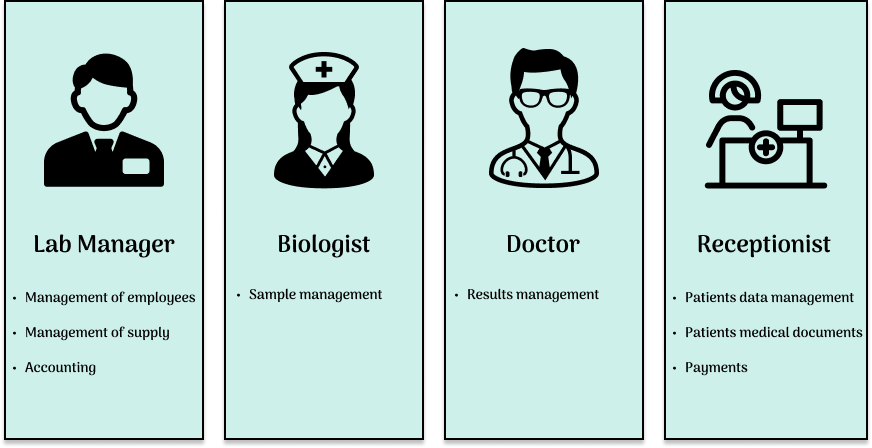
\includegraphics[width=451px]{media/stakeholders.png}
    \captionof{figure}{Stakeholders and their specifications}
\end{center}

\subsubsection*{Laboratory Manager:}

The laboratory manager is responsible for the overall management of the laboratory. He is responsible for the management of employees, supply, and accounting.

\noindent The functionalities needed by the laboratory manager are:

\begin{itemize}

\item \textbf{Management of employees:} a system for the management of the roles and privileges of each employee and the resources they can access. An employee is defined by (ID, Name, Role, Username, Password, Phone, Email).

\item \textbf{Management of supply:} the ability to check, and control (add, modify and remove) the many equipments (tubes, reagents \ldots) that are used on a daily basis.

\item \textbf{Accounting:} a system to keep track of the different spendings and earnings of the lab.

\end{itemize}


\subsubsection*{Biologist:}

The biologist is responsible for the process of sample analysis. He takes the collected samples and runs the required tests on them. He then inserts the obtained results into the system.

\noindent The functionalities needed by the biologist are:

\begin{itemize}
    \item \textbf{Sample management:} the ability to view, add, modify the sample test results of patients on and from the database.
\end{itemize}

\subsubsection*{Doctor:}

The doctor is responsible for viewing and checking the validity of the  test results conducted by the biologist.

\noindent The functionalities needed by the doctor are:

\begin{itemize}

\item \textbf{Results validity management:} the ability to view the results of each patient's test and choose to validate those results for final delivery or not.

\end{itemize}


\subsubsection*{Receptionist:}

The receptionist is responsible for the management of patients' data, medical history, and payments.

\noindent The functionalities needed by the receptionist are:

\begin{itemize}

\item \textbf{Patients data management:} a system for storing and manipulating patients data. It should provide the ability to add new patients and to modify or delete existing ones.

\item \textbf{Patients medical documents:} the ability to input and keep track of patient's medical history and sample test results.

\item \textbf{Patients payments:} keeps track of the payment situation of each patient and provides essential information about it.

\end{itemize}

\subsection[Conclusion]{Conclusion}
In this section we were able to construct a descriptive scenario of the daily workflow in a medical laboratory. We used this scenario to identify the different stakeholders and their needs. We then specified the functionalities needed by each stakeholder. In the next section, we will use this information to inform our design choices and to develop the application.


\newpage
\section{Application Design}

\subsection[Introduction]{Introduction}

In engineering, the design phase is aimed at formalizing the preliminary stages of developing a system to make this development more faithful to the client's needs.

Design is a crucial step in the development of any software application. It is the process of describing the architecture, components, modules, interfaces, and data for a system to satisfy specified requirements. It is the bridge between requirements analysis and implementation.

Its goal is to describe unambiguously, often using a modeling language, the future operation of the system to facilitate its implementation.

There are two main approaches to designing information systems: the functional approach and the object-oriented approach. The functional approach perceives the system as an entity performing a global function that can be broken down into sub-functions. The object-oriented approach views the system as a set of objects interacting with each other. 

In our work, we have opted for the object-oriented approach, which ensures software evaluation and object realization, which is not guaranteed with simplified modeling and development methods.

\subsection[Unified Modeling Language]{Unified Modeling Language}

Unified Modeling Language (UML) is a standardized modeling language used in software engineering for visualizing, specifying, constructing, and documenting the artifacts of a software-intensive system. It is a graphical language that provides a common vocabulary and set of diagrams to describe software systems.

\subsection[Why UML?]{Why UML?}

\begin{itemize}
    \item \textbf{Visual Representation:} UML provides a visual representation of the system which is easy to understand and interpret.
    \item \textbf{Standardization:} UML is a standardized language for specifying, visualizing, constructing, and documenting the artifacts of software systems. This standardization helps in maintaining consistency across different projects.
    \item \textbf{Communication:} UML diagrams facilitate effective communication among team members and stakeholders. They provide a common language that all parties involved can understand, reducing the chances of miscommunication.
    \item \textbf{Design Validation:} UML diagrams can be used to validate the design of the system. They can help identify potential issues or flaws in the design before the implementation phase.
    \item \textbf{Documentation:} UML diagrams serve as a form of documentation for the system. They can be used as a reference for future development or maintenance activities.
    \item \textbf{Modularity:} UML promotes modularity and separation of concerns by allowing the design to be broken down into different diagrams each focusing on a specific aspect of the system.
    \item \textbf{Platform Independent:} UML is platform independent. It can be used to design systems irrespective of the programming languages and platforms used for implementation.
\end{itemize}

\subsection[Diagrams]{Diagrams}
\subsubsection*{Use Case Diagram:}

\paragraph*{\textbf{Definition:} }

Use case diagrams are a type of behavior diagram in UML that represent the functional requirements of a system from the perspective of its users. They show the interactions between the system and its actors (users or external systems) by depicting the various use cases (functions or services) that the system provides. Use case diagrams help in identifying, organizing, and prioritizing the functionalities of a system and are often used during the requirements' analysis phase of software development.

\paragraph*{\textbf{Purpose: }}
\begin{itemize}
    \item Define the limits of the system.
    \item Define the system environment: the users and elements that interact with the system.
    \item Define the fundamental usages of the system.
\end{itemize}

\paragraph*{\textbf{Diagram Elements: }}
\vspace{0.3cm}
\begin{center}
    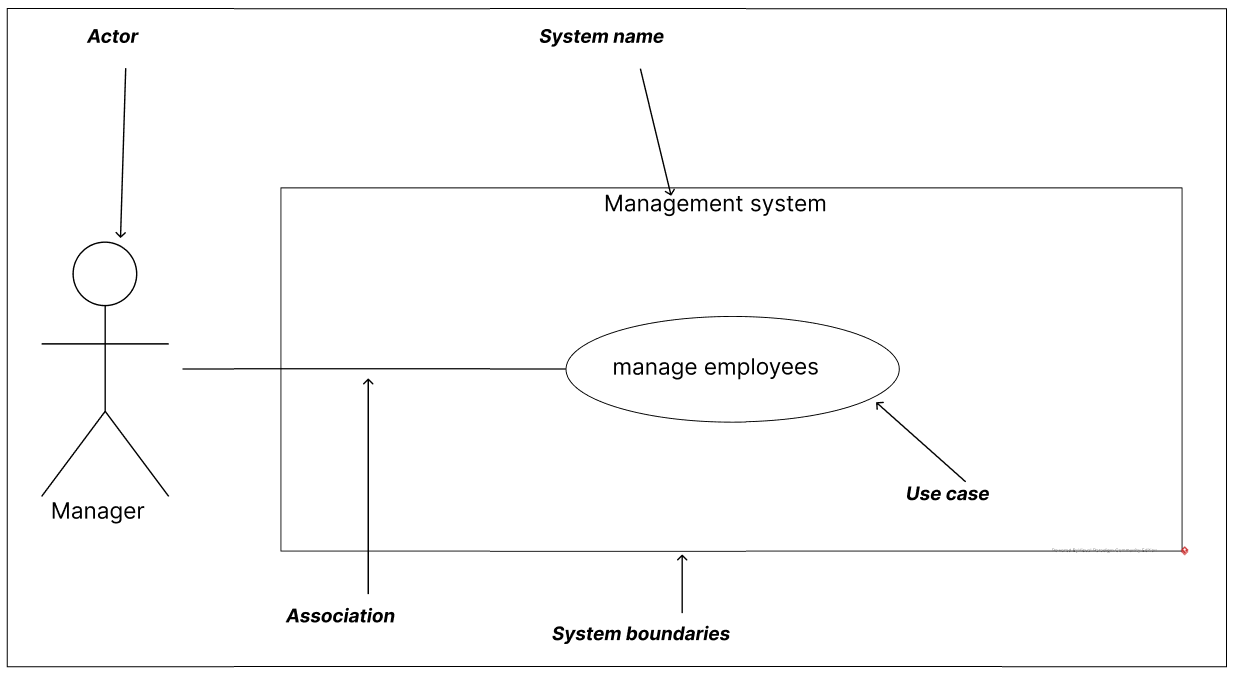
\includegraphics[width=451px]{media/use_case_elements.png}
    \captionof{figure}{Use Case Diagram Elements}
\end{center}


\begin{itemize}
    \item \textbf{Actor:} An actor represents a role played by a user or any other system that interacts with the system. Actors are drawn as stick figures and are connected to use cases by lines.
    \begin{center}
        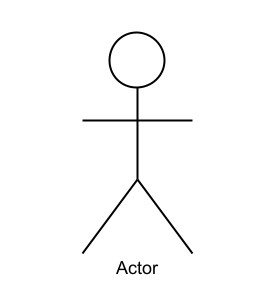
\includegraphics[width=100px]{media/actor.jpg}
        \captionof{figure}{Representation of "Actor" in a Use Case Diagram}
    \end{center}
    \item \textbf{Use Case:} A use case represents a specific functionality or service provided by the system. It describes the interactions between the system and its actors to achieve a specific goal. Use cases are drawn as ovals and are connected to actors by lines.
    \begin{center}
        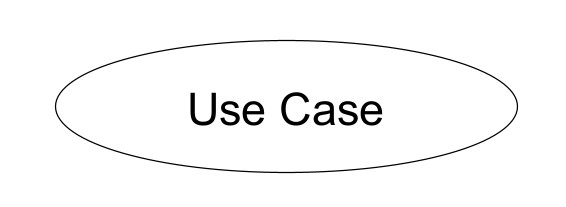
\includegraphics[width=100px]{media/use_case.jpg}
        \captionof{figure}{Representation of "Use Case" in a Use Case Diagram}
    \end{center}
    \item \textbf{Associations:} There are three types:
    \begin{itemize}
        \item Between actor and use case: it is simple, connecting an actor and its functionalities.
        \item Between two use cases: connecting two use cases have a correspondence. Represented in tree forms depending on the case; (specialization/generalization, inclusion, extension).
        \begin{center}
            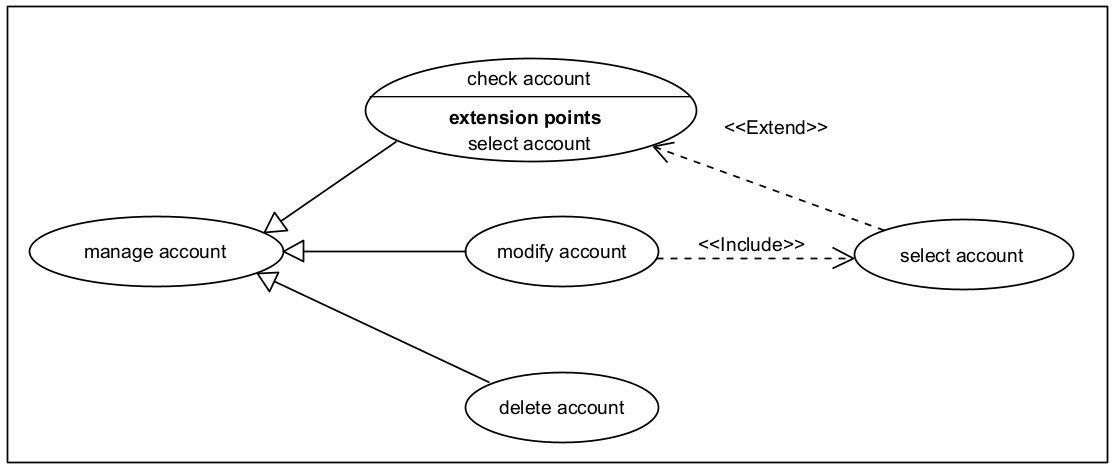
\includegraphics[width=400px]{media/use_case_relations.jpg}
            \captionof{figure}{Different types of associations in a Use Case Diagram}
        \end{center}
        \item Between actors: connects two actors, having an inheritance relationship between them.
        \begin{center}
            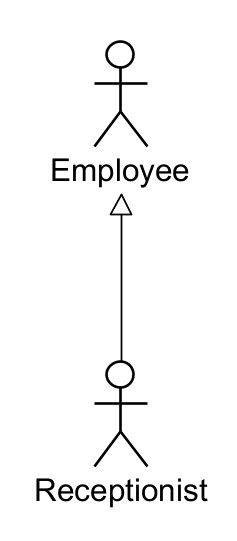
\includegraphics[width=60px]{media/inheritence.jpg}
            \captionof{figure}{Association between two actors in a Use Case Diagram}
        \end{center}  
    \end{itemize}
\end{itemize}

In our project, we opted for using a structured Use Case Diagram for each actor of the system.

\begin{center}
    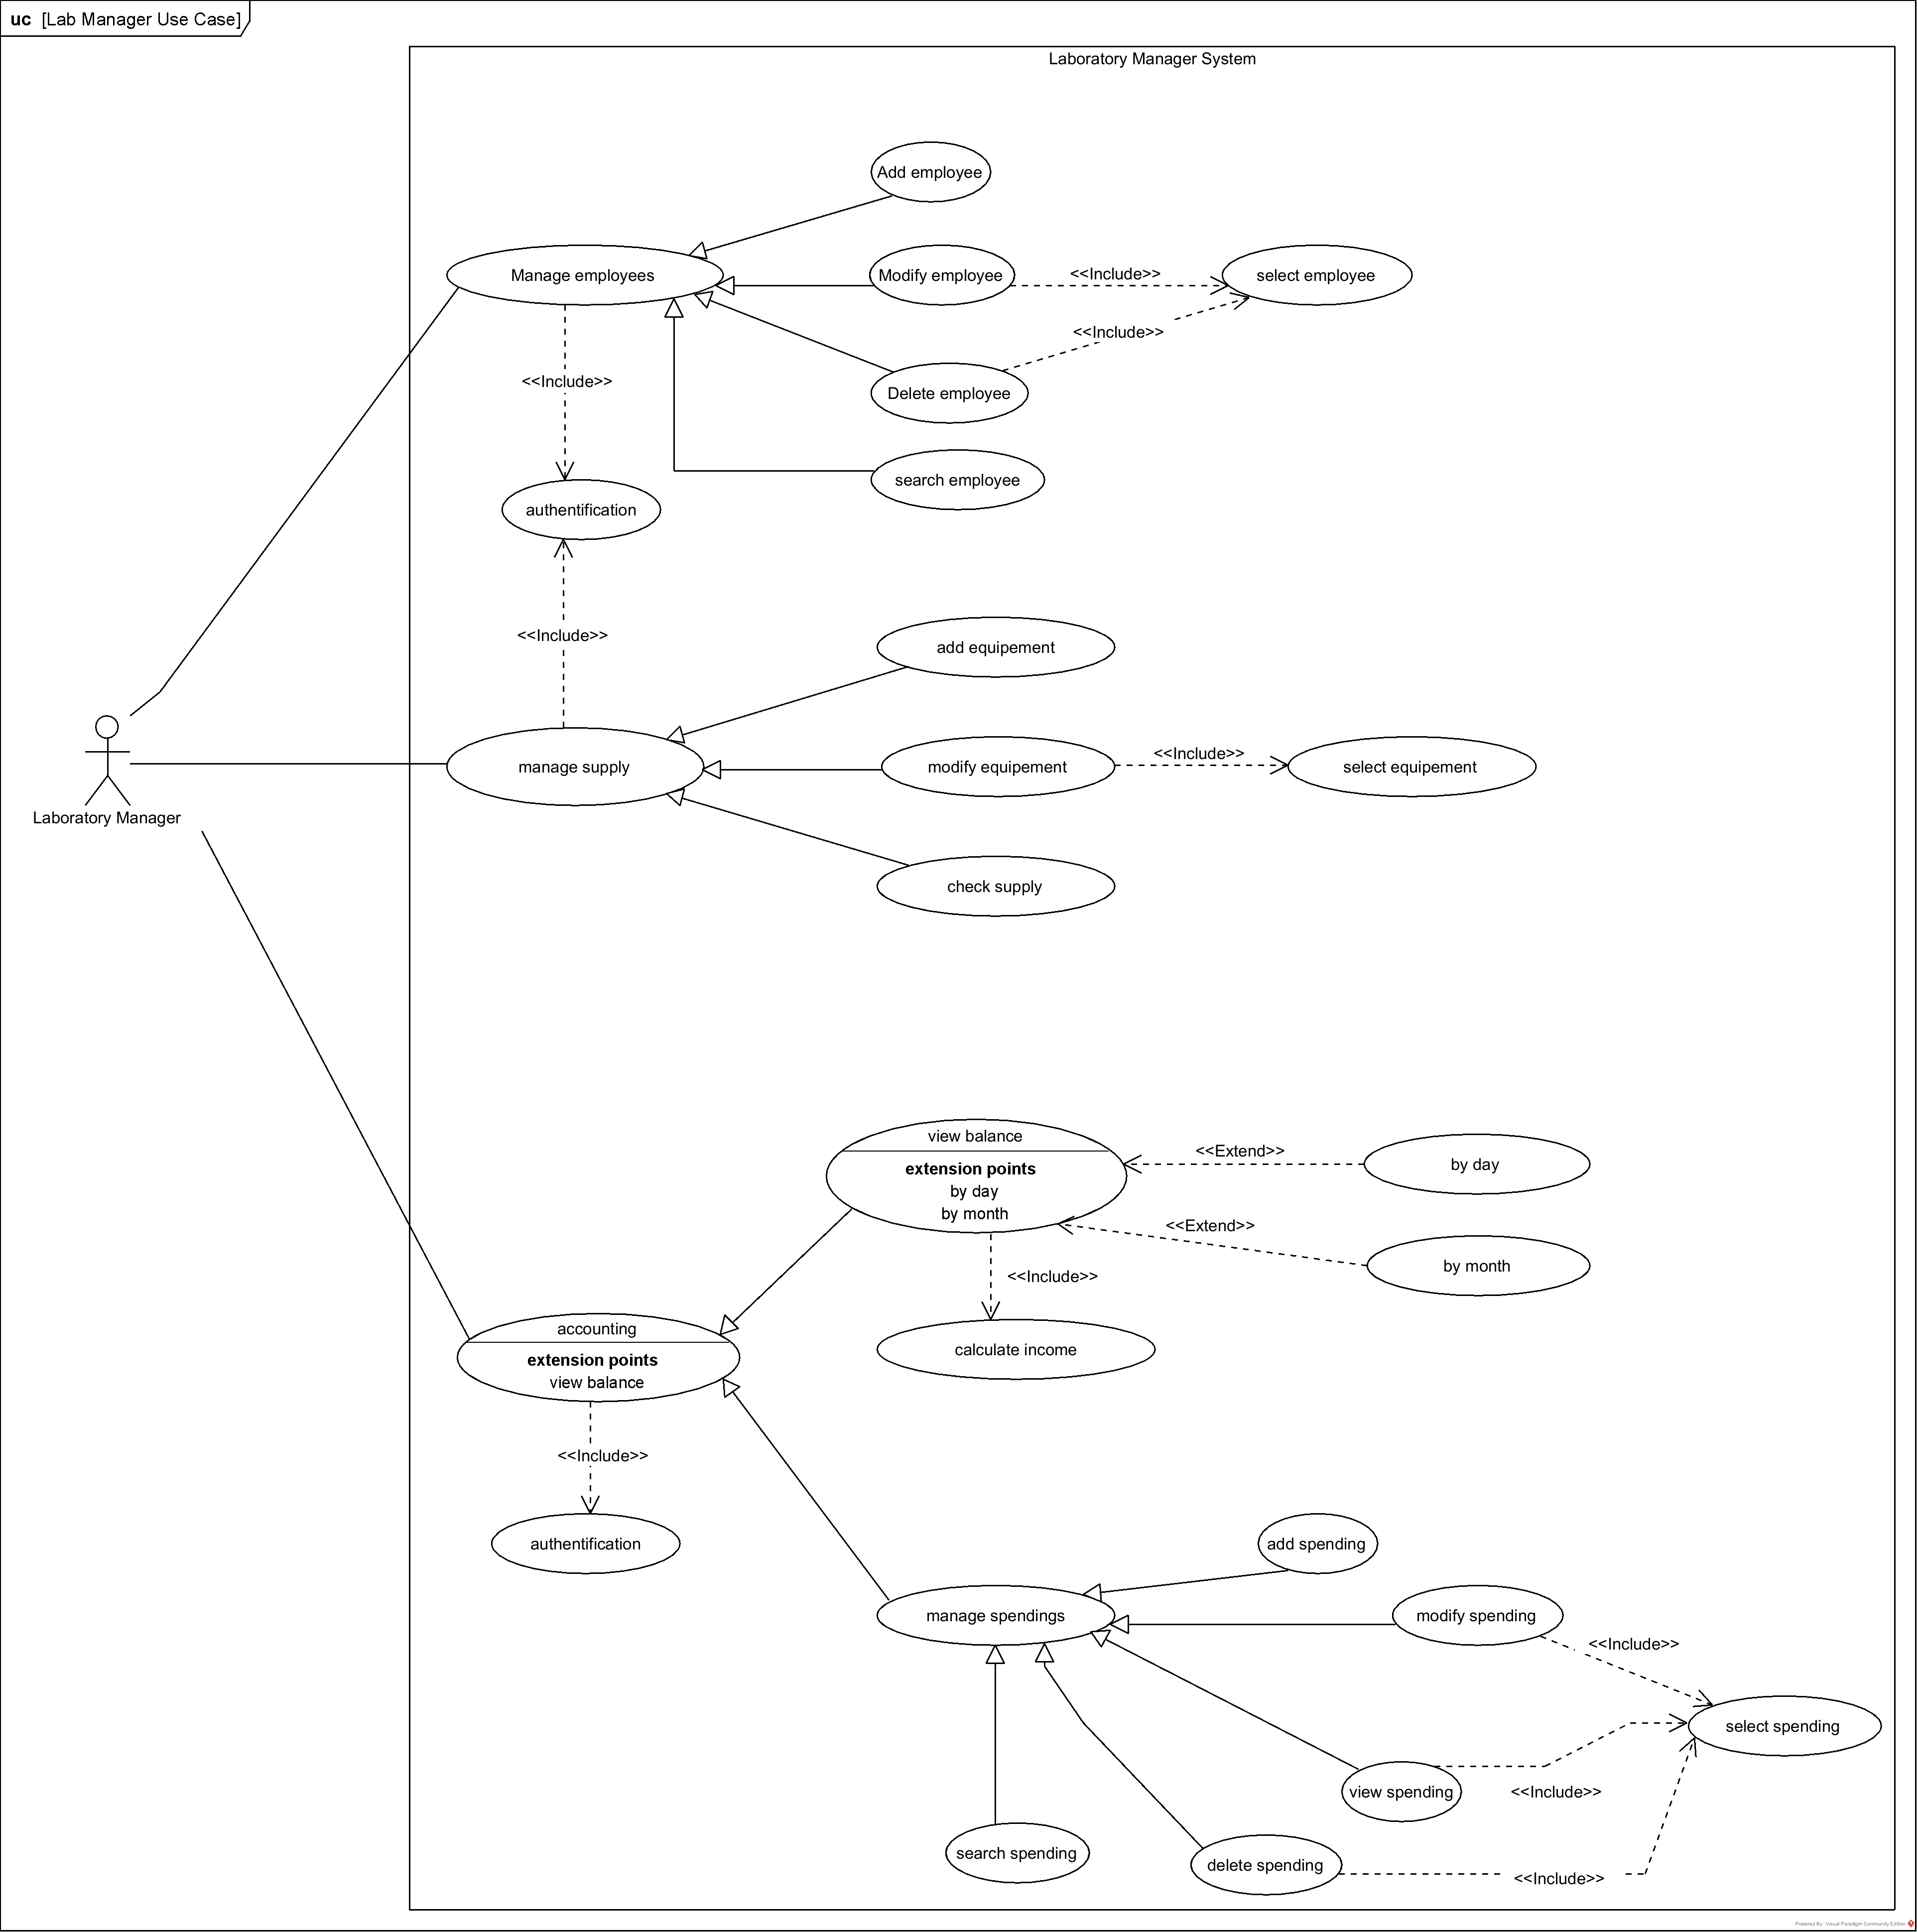
\includegraphics[width=451px]{media/Use case diagrams/Lab Manager Use Case.png}
    \captionof{figure}{Use Case Diagram for the Laboratory Manager}
\end{center}


\begin{center}
    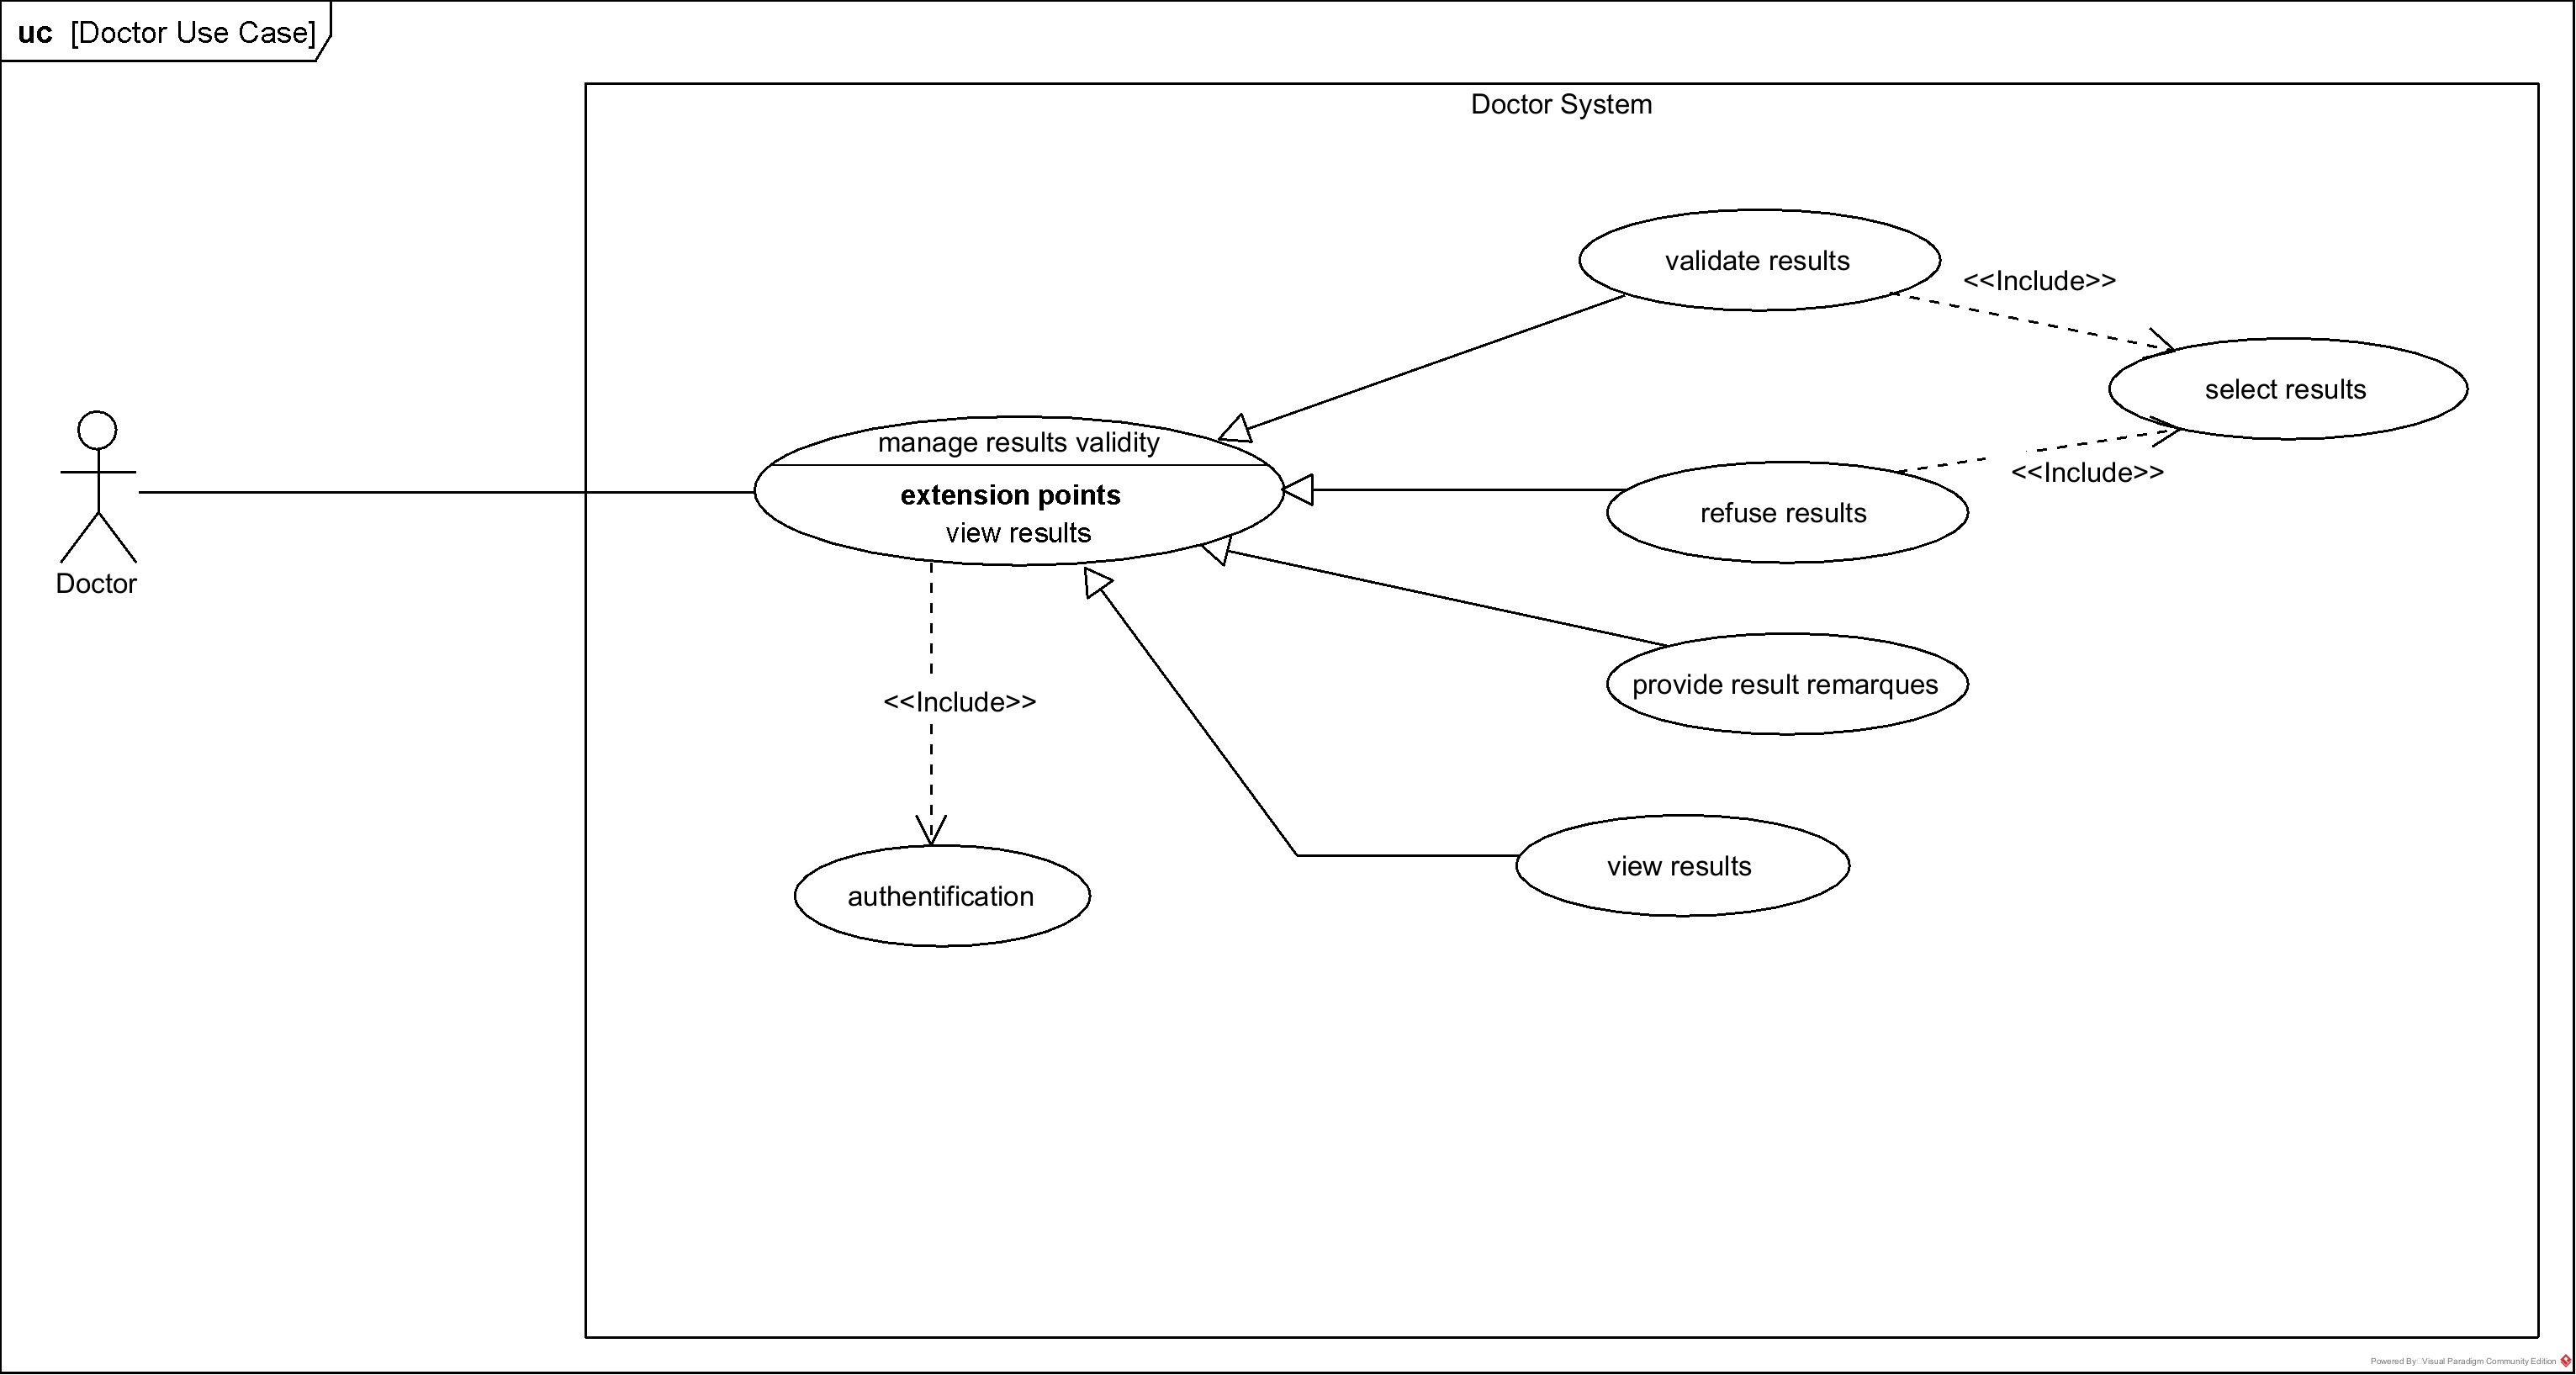
\includegraphics[width=451px]{media/Use case diagrams/Doctor Use Case.png}
    \captionof{figure}{Use Case Diagram for the Doctor}
\end{center}



\begin{center}
    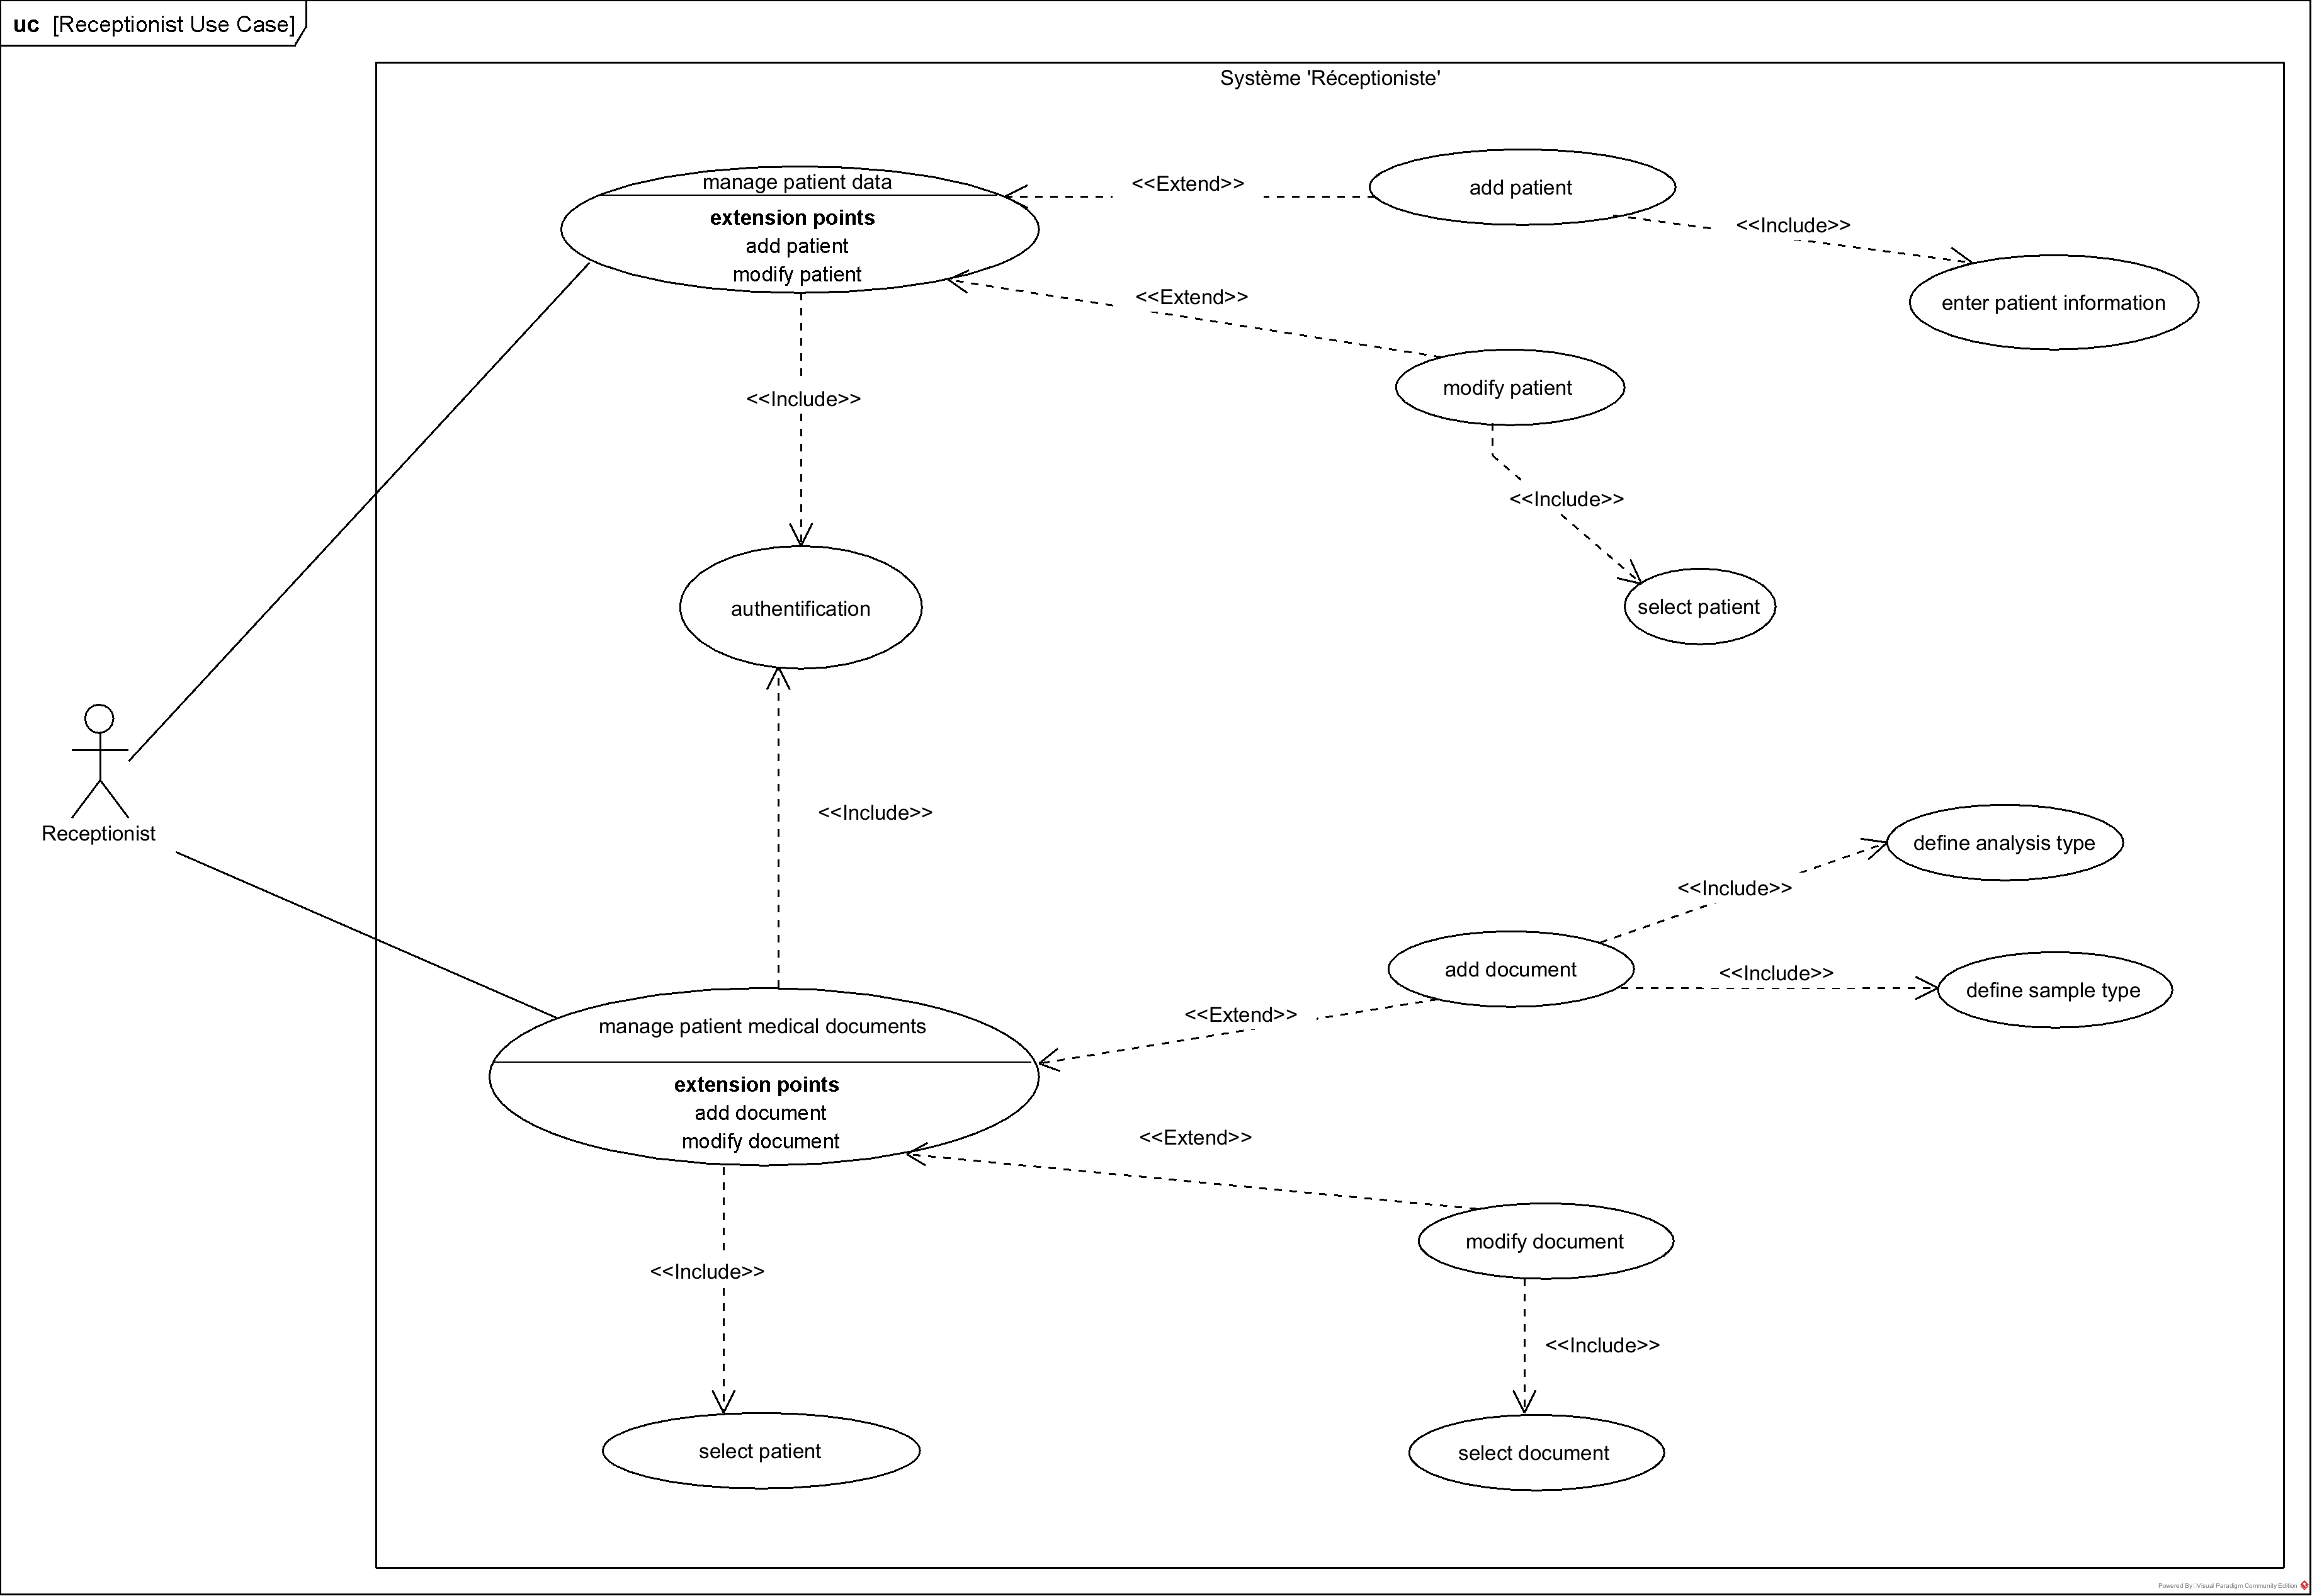
\includegraphics[width=451px]{media/Use case diagrams/Receptionist Use Case.png}
    \captionof{figure}{Use Case Diagram for the Receptionist}
\end{center}


\begin{center}
    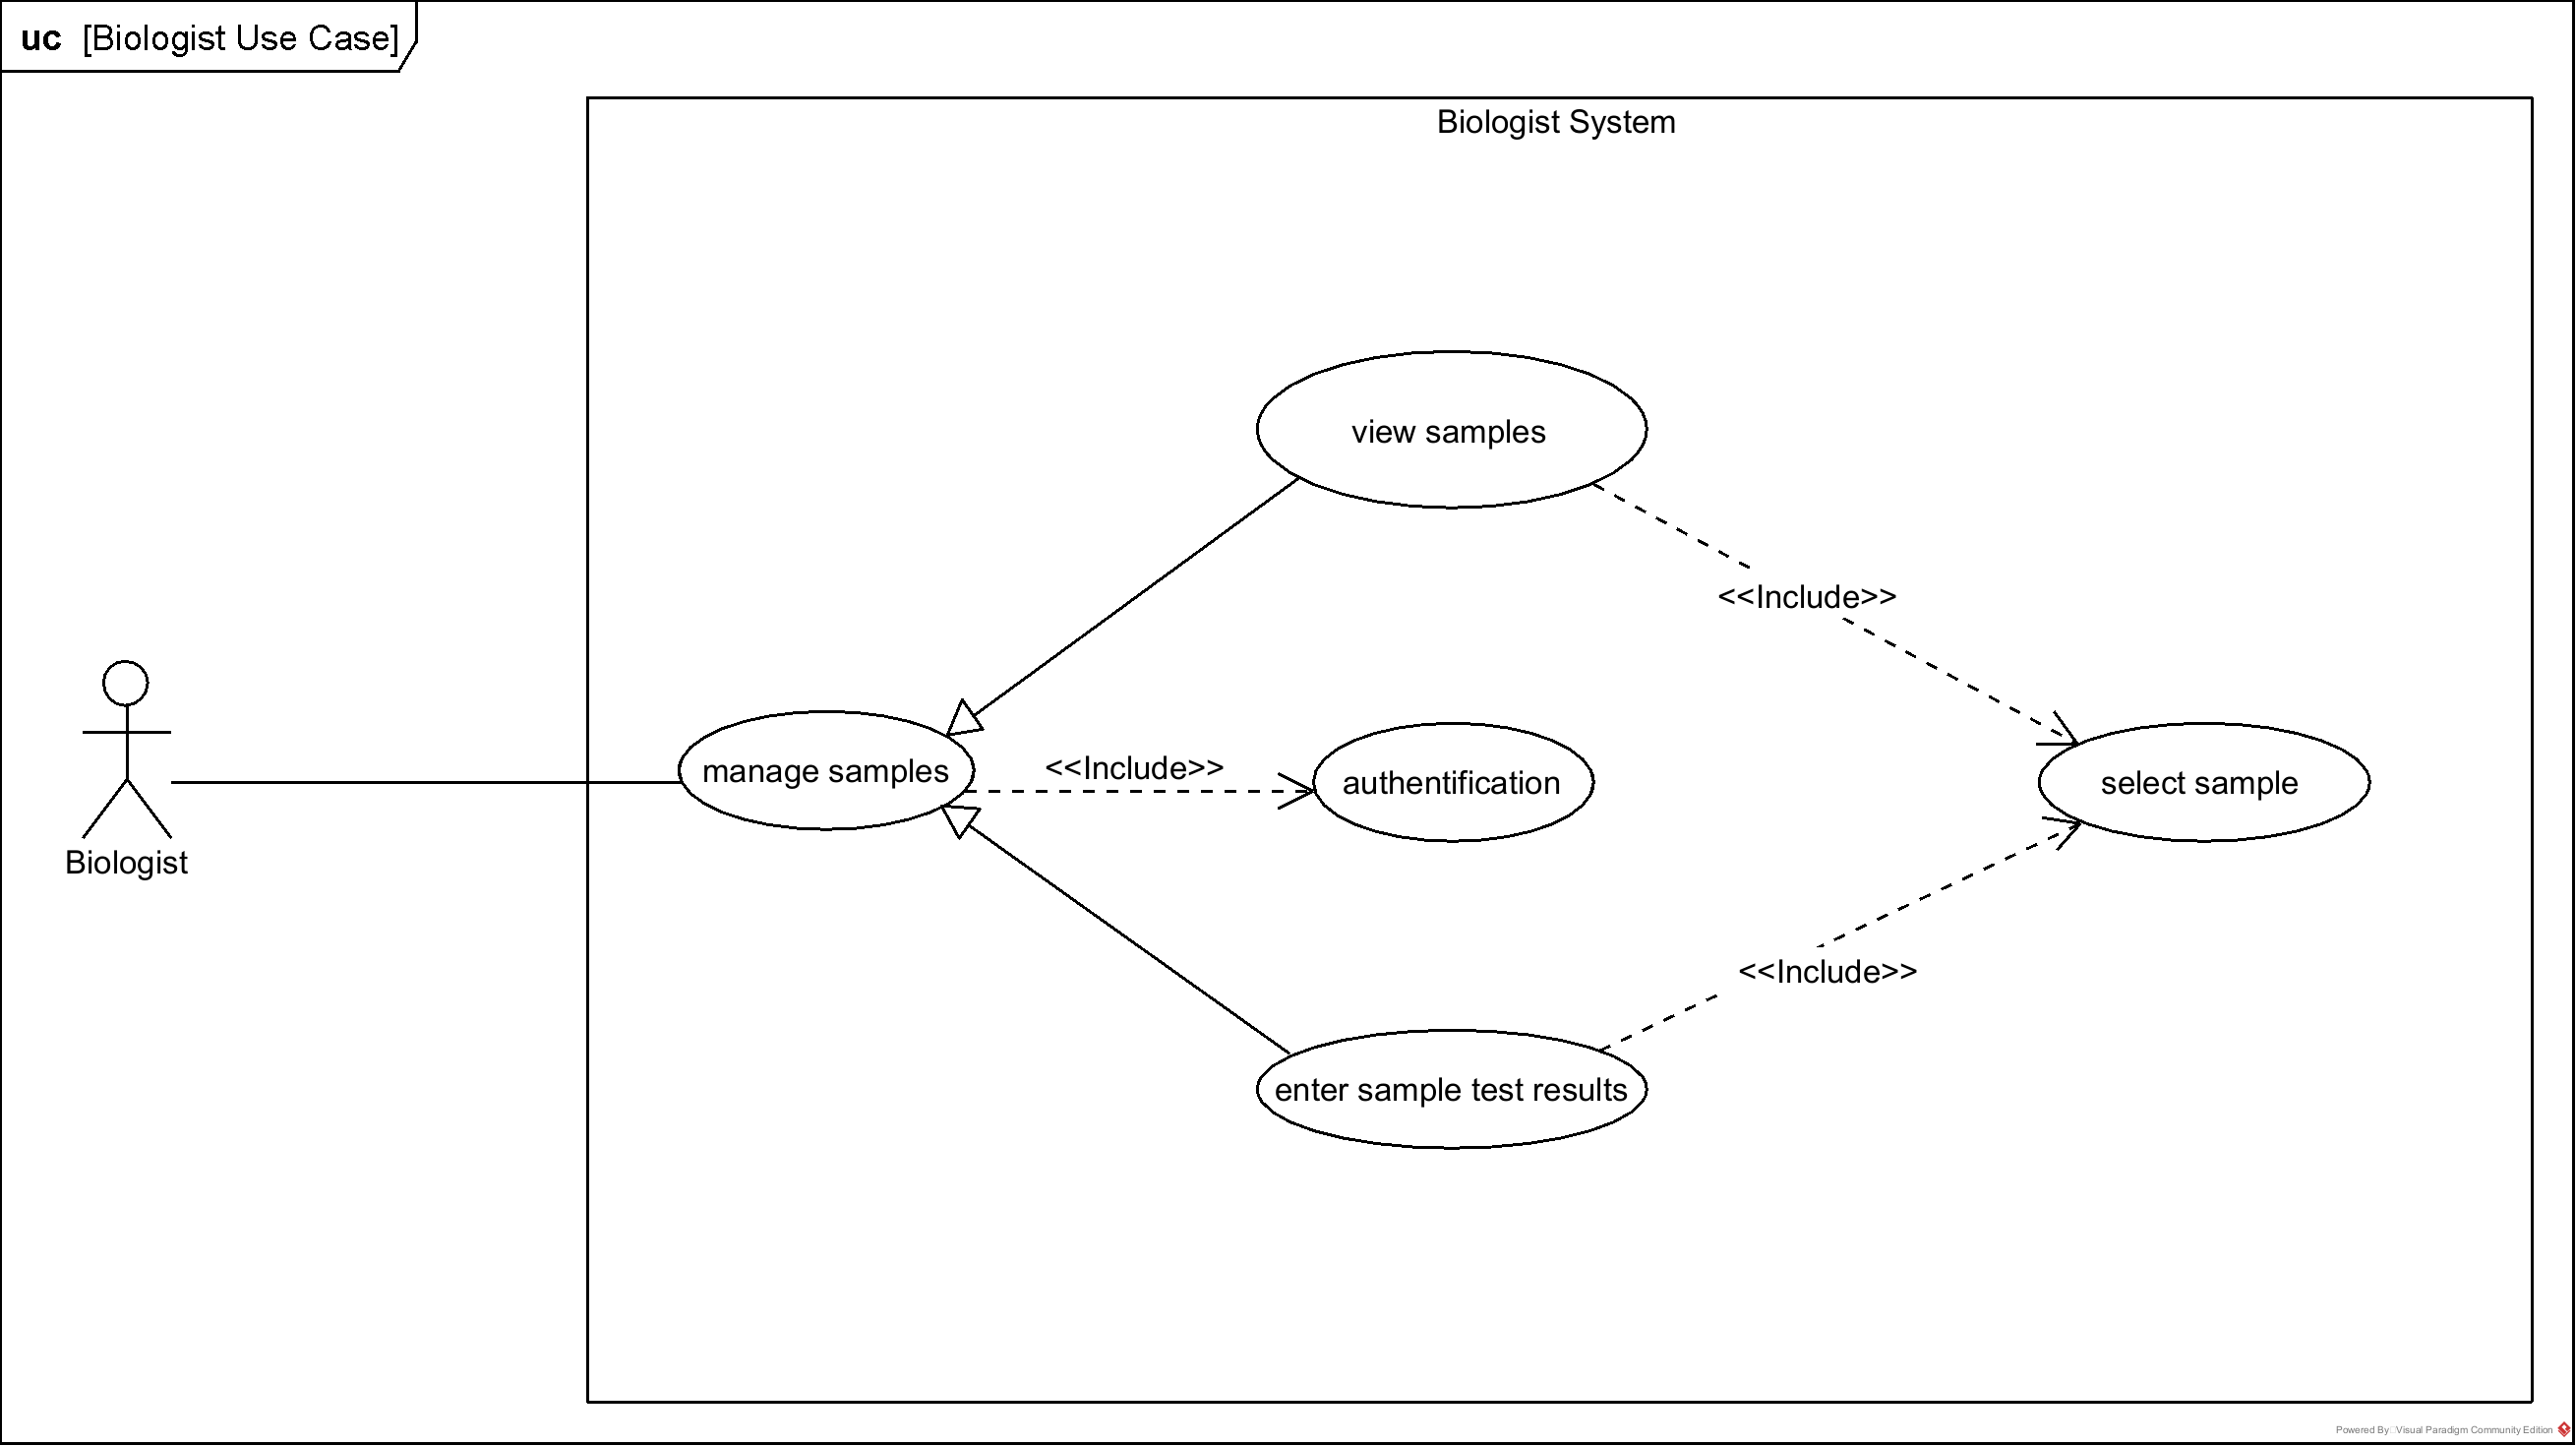
\includegraphics[width=451px]{media/Use case diagrams/Biologist Use Case.png}
    \captionof{figure}{Use Case Diagram for the Biologist}
\end{center}


\newpage
\subsubsection*{Descriptive Cards of Use Cases}

The description of a Use Case is a narrative document that describes the sequence of interactions in which the actor uses the system to arrive at a result that satisfies the initial purpose of the Use Case.

\noindent\paragraph*{Here are our descriptive cards for the main use cases:}

\textbf{Descriptive Card for "Authentication":}

\begin{table}[h]
\setlength{\tabcolsep}{10pt}
\renewcommand{\arraystretch}{1.5}
    \begin{tabular}{|p{\linewidth}|}
        \hline
        \textbf{Use Case Name:} Authentication\\ 
        \hline
        \textbf{Type:} Secondary\\ 
        \hline
        \textbf{Actor:} Laboratory manager, Biologist, Doctor, Receptionist\\ 
        \hline
        \textbf{Purpose:} Allows the actors to access their respective application interface, the user needs to enter their user name and password, then the system checks if the credentials are correct or not for the purpose of giving or denying their access request.\\ 
        \hline
        \textbf{Precondition:} The user already has an account.\\ 
        \hline
        \textbf{Scenario:}
        \vspace{0.2cm}
        \newline
        \vspace{0.2cm}
        \textbf{Start Action:} The user starts the application and is welcomed by the login interface.
        \newline
        \textbf{Ongoing Action:}  
        \begin{itemize}
            \item The user enters their username and password and clicks on the login button.
            \item The system checks the credentials.
            \item The system grants or denies access.
        \end{itemize}
        \textbf{Final Action:} The system redirects the user to their interface.\\
        \hline
        \textbf{Alternative:} 
        \begin{itemize}
            \item The user enters incorrect credentials.
            \item The login fields are empty.
        \end{itemize}\\ 
        \hline
        \textbf{Exception:}
        \begin{itemize}
            \item the user is not registered.
            \item cancellation of the login.
        \end{itemize}\\ 
        \hline
    \end{tabular}
    \caption{Descriptive Card for "Authentication"}
    \label{tab:my-table}
\end{table}


\newpage

\textbf{Descriptive Card for "Add employee":}

\begin{table}[h]
\setlength{\tabcolsep}{10pt}
\renewcommand{\arraystretch}{1.5}
    \begin{tabular}{|p{\linewidth}|}
        \hline
        \textbf{Use Case Name:} Add employee\\ 
        \hline
        \textbf{Type:} Primary\\ 
        \hline
        \textbf{Actor:} Laboratory manager\\ 
        \hline
        \textbf{Purpose:} Allows the laboratory manager to add a new employee (user) to the system along with their information.\\ 
        \hline
        \textbf{Precondition:} 
        \begin{itemize}
            \item The laboratory manager is logged in.
        \end{itemize}\\ 
        \hline
        \textbf{Scenario:}
        \vspace{0.2cm}
        \newline
        \vspace{0.2cm}
        \textbf{Start Action:} The laboratory manager clicks on the "Add employee" button.
        \newline
        \textbf{Ongoing Action:}  
        \begin{itemize}
            \item The laboratory manager fills in the employee's information (ID, Name, Role, Username, Password, Phone, Email).
            \item the laboratory manager clicks on the "Add" button.
            \item The system adds the employee to the database.
        \end{itemize}
        \textbf{Final Action:} The system confirms the operation by displaying the new list of existing employees\\
        \hline
        \textbf{Alternative:} 
        \begin{itemize}
            \item the employee already exists.
            \item the fields are empty.
        \end{itemize}\\ 
        \hline
        \textbf{Exception:}
        \begin{itemize}
            \item the operation is canceled.
        \end{itemize}\\ 
        \hline
    \end{tabular}
    \caption{Descriptive Card for "Add employee"}
    \label{tab:my-table}
\end{table}

\newpage

\textbf{Descriptive Card for "Search employee":}

\begin{table}[h]
\setlength{\tabcolsep}{10pt}
\renewcommand{\arraystretch}{1.5}
    \begin{tabular}{|p{\linewidth}|}
        \hline
        \textbf{Use Case Name:} Search employee\\ 
        \hline
        \textbf{Type:} Primary\\ 
        \hline
        \textbf{Actor:} Laboratory manager\\ 
        \hline
        \textbf{Purpose:} The purpose of the employee search in a laboratory analysis system is to provide quick, accurate, and secure access to employee information and to verify their existence in the system.\\ 
        \hline
        \textbf{Precondition:}
        \begin{itemize}
            \item The laboratory manager is logged in.
            \item The employee exists in the system.
        \end{itemize}
        \\ 
        \hline
        \textbf{Scenario:}
        \vspace{0.2cm}
        \newline
        \vspace{0.2cm}
        \textbf{Start Action:} The laboratory manager clicks on the search bar.
        \newline
        \textbf{Ongoing Action:}  
        \begin{itemize}
            \item The laboratory manager enters the employee's name or ID.
            \item The system filters the list of employees.
        \end{itemize}
        \textbf{Final Action:} the system displays the employee information.\\
        \hline
        \textbf{Alternative:} 
        \begin{itemize}
            \item incorrect employee name or ID.
            \item empty search bar.
        \end{itemize}\\ 
        \hline
        \textbf{Exception:}
        \begin{itemize}
            \item the operation is canceled. 
        \end{itemize}\\ 
        \hline
    \end{tabular}
    \caption{Descriptive Card for "Search employee"}
    \label{tab:my-table}
\end{table}

\newpage

\textbf{Descriptive Card for "Modify equipment":}

\begin{table}[h]
\setlength{\tabcolsep}{10pt}
\renewcommand{\arraystretch}{1.5}
    \begin{tabular}{|p{\linewidth}|}
        \hline
        \textbf{Use Case Name:} Modify equipment\\ 
        \hline
        \textbf{Type:} Primary\\ 
        \hline
        \textbf{Actor:} Laboratory Manager\\ 
        \hline
        \textbf{Purpose:} Allows the laboratory manager to change the information of an existing equipment in the supply management interface. It allows the modification of the equipment's name, quantity and type.\\ 
        \hline
        \textbf{Precondition:}
        \begin{itemize}
            \item the laboratory manager is logged in.
            \item the equipment already exists.
        \end{itemize}\\ 
        \hline
        \textbf{Scenario:}
        \vspace{0.2cm}
        \newline
        \vspace{0.2cm}
        \textbf{Start Action:} the laboratory manager select the equipment and clicks the "modify" button.
        \newline
        \textbf{Ongoing Action:}  
        \begin{itemize}
            \item the laboratory manager enter the new information in the appropriate fields
            \item the laboratory manager clicks the "save" button.
            \item the system updates the equipment's existing information.
        \end{itemize}
        \textbf{Final Action:} the system displays the new product's information \\
        \hline
        \textbf{Alternative:} 
        \begin{itemize}
            \item the entered information type is not compatible.
        \end{itemize}\\ 
        \hline
        \textbf{Exception:}
        \begin{itemize}
            \item the operation is canceled. 
        \end{itemize}\\ 
        \hline
    \end{tabular}
    \caption{Descriptive Card for "Modify equipment"}
    \label{tab:my-table}
\end{table}

\newpage

\textbf{Descriptive Card for "View Balance":}

\begin{table}[h]
\setlength{\tabcolsep}{10pt}
\renewcommand{\arraystretch}{1.5}
    \begin{tabular}{|p{\linewidth}|}
        \hline
        \textbf{Use Case Name:} View Balance\\ 
        \hline
        \textbf{Type:} Primary\\ 
        \hline
        \textbf{Actor:} Laboratory Manager\\ 
        \hline
        \textbf{Purpose:} Allows the laboratory manager to view the flow of income and spendings of the laboratory, as well as view the calculated net income.\\ 
        \hline
        \textbf{Precondition:}
        \begin{itemize}
            \item the laboratory manager is logged in.
        \end{itemize}\\ 
        \hline
        \textbf{Scenario:}
        \vspace{0.2cm}
        \newline
        \vspace{0.2cm}
        \textbf{Start Action:} Clicks on the "Finance" option in the side bar
        \newline
        \textbf{Ongoing Action:}  
        \begin{itemize}
            \item the system displays the spendings and income transactions 
        \end{itemize}
        \textbf{Final Action:} The system calculate the net income and displays it to the user. \\
        \hline
        \textbf{Alternative:} 
        \begin{itemize}
            \item there are no transactions yet.
        \end{itemize}\\ 
        \hline
        \textbf{Exception:} //\\ 
        \hline
    \end{tabular}
    \caption{Descriptive Card for "View Balance"}
    \label{tab:my-table}
\end{table}

\newpage
\textbf{Descriptive Card for "Add patient medical document":}

\begin{table}[h]
\setlength{\tabcolsep}{10pt}
\renewcommand{\arraystretch}{1.5}
    \begin{tabular}{|p{\linewidth}|}
        \hline
        \textbf{Use Case Name:} Add document\\ 
        \hline
        \textbf{Type:} Primary\\ 
        \hline
        \textbf{Actor:} Receptionist\\ 
        \hline
        \textbf{Purpose:} Allows the creation of a request for a medical test document associated with a patient which describes their analysis and their price; the receptionist must choose a patient then add their required analysis, and finally save the document to the database.
        \\ 
        \hline
        \textbf{Precondition:}
        \begin{itemize}
            \item the receptionist is logged in.
            \item  Patient already exists in the database.
        \end{itemize}
       \\ 
        \hline
        \textbf{Scenario:}
        \vspace{0.2cm}
        \newline
        \vspace{0.2cm}
        \textbf{Start Action:} The Receptionist clicks on the "New" button.
        \newline
        \textbf{Ongoing Action:}  
        \begin{itemize}
            \item The system shows a window which contains the list of patients.
            \item The receptionist chooses a patient.
            \item the system shows the list of available analysis.
            \item The receptionist chooses the analysis.
            \item The receptionist clicks on the "Save" button.
            \item the system calculates the price.
        \end{itemize}
        \textbf{Final Action:} the system saves the test request and relevant information in the database.\\
        \hline
        \textbf{Alternative:} 
        \begin{itemize}
            \item the patient or the analysis does not exist.
        \end{itemize}\\ 
        \hline
        \textbf{Exception:}
        \begin{itemize}
            \item the operation is canceled. 
        \end{itemize}\\ 
        \hline
    \end{tabular}
    \caption{Descriptive Card for "Add document"}
    \label{tab:my-table}
\end{table}

\newpage

\textbf{Descriptive Card for "Validate Results":}

\begin{table}[h]
\setlength{\tabcolsep}{10pt}
\renewcommand{\arraystretch}{1.5}
    \begin{tabular}{|p{\linewidth}|}
        \hline
        \textbf{Use Case Name:} Validate Results\\ 
        \hline
        \textbf{Type:} Primary\\ 
        \hline
        \textbf{Actor:} Doctor\\ 
        \hline
        \textbf{Purpose:} Allows the doctor to be able to validate the analysis results that are submitted by the biologist.
        It ensures the credibility of the results.\\ 
        \hline
        \textbf{Precondition:}
        \begin{itemize}
            \item the doctor is logged in.
            \item The results have been submitted by the biologist.
            \item the doctor has the results code.
        \end{itemize}\\ 
        \hline
        \textbf{Scenario:}
        \vspace{0.2cm}
        \newline
        \vspace{0.2cm}
        \textbf{Start Action:} The doctor select the search bar.
        \newline
        \textbf{Ongoing Action:}  
        \begin{itemize}
            \item The doctor enters the results code.
            \item The doctor checks the validity of the results.
            \item the doctor enters a comment.
            \item The doctor clicks on the "Validate" or "Refuse" button.
        \end{itemize}
        \textbf{Final Action:} The system saves the validation information.\\
        \hline
        \textbf{Alternative:} 
        \begin{itemize}
            \item the results code is incorrect.
        \end{itemize}\\ 
        \hline
        \textbf{Exception:}
        \begin{itemize}
            \item the operation is canceled. 
        \end{itemize}\\ 
        \hline
    \end{tabular}
    \caption{Descriptive Card for "Validate Results"}
    \label{tab:my-table}
\end{table}



\newpage
\subsubsection*{Sequence Diagram:}

\paragraph*{\textbf{Definition:} }

A sequence diagram is a Unified Modeling Language (UML) diagram that represents the sequence of messages between objects during an interaction.


\paragraph*{\textbf{Purpose: }}
\begin{itemize}
    \item Describes the implementation of use cases on the system described by the class diagram.
    \item An internal point of view into the system functions.
    \item Description at a momentary level (system state at a given moment).
    \item Representation of messages exchange.
\end{itemize}

\paragraph*{\textbf{Diagram Elements: }}
\vspace{0.3cm}
\begin{center}
    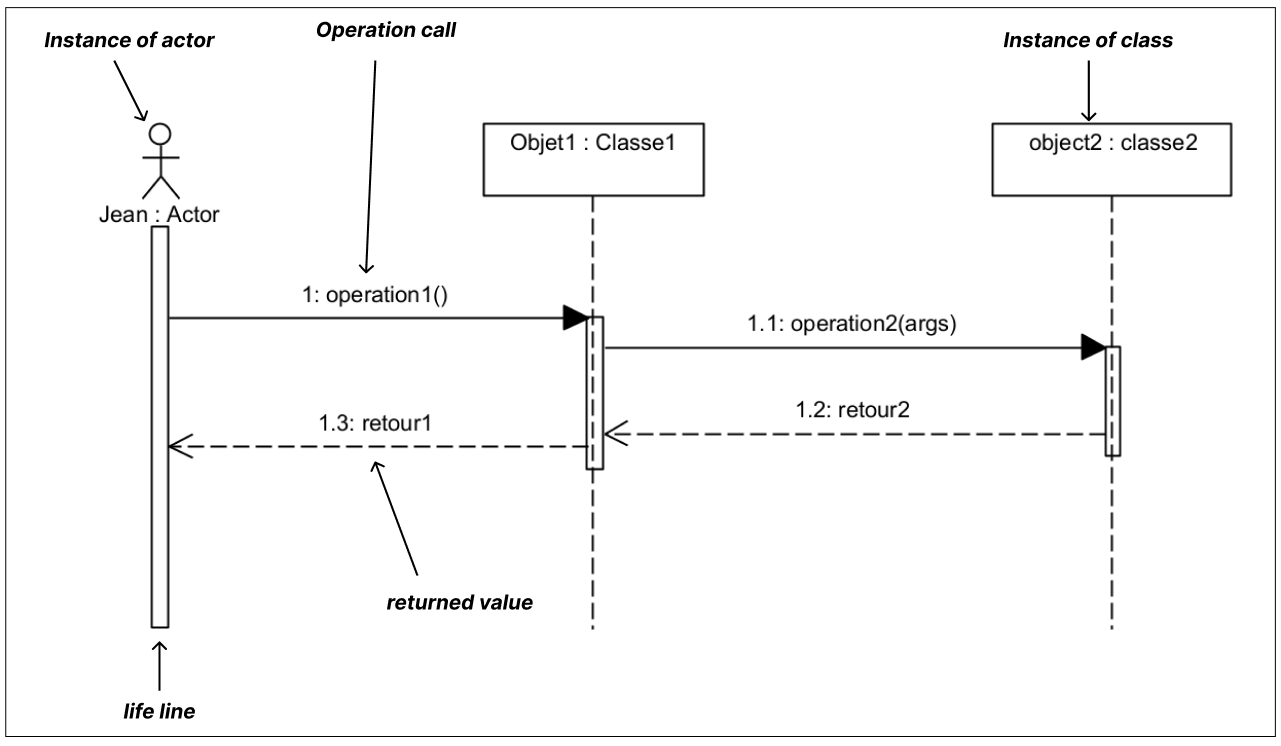
\includegraphics[width=451px]{media/sequence_elements.png}
    \captionof{figure}{Sequence Diagram Elements}
\end{center}

\paragraph*{\textbf{Different Operation Types:}}
\begin{itemize}
    \item Alternative: Conditional message sending.
    \item Reference: Reference of an external diagram.
    \item Break: An exception raised.
    \item Loop: Repeat a sequence of messages.
\end{itemize}
\vspace{1cm}
\noindent Here are our Sequence Diagrams for the main functionalities of the system:


\newpage
This Sequence Diagram represents the interactions between the user and the system to obtain an access authorization.

\begin{center}
    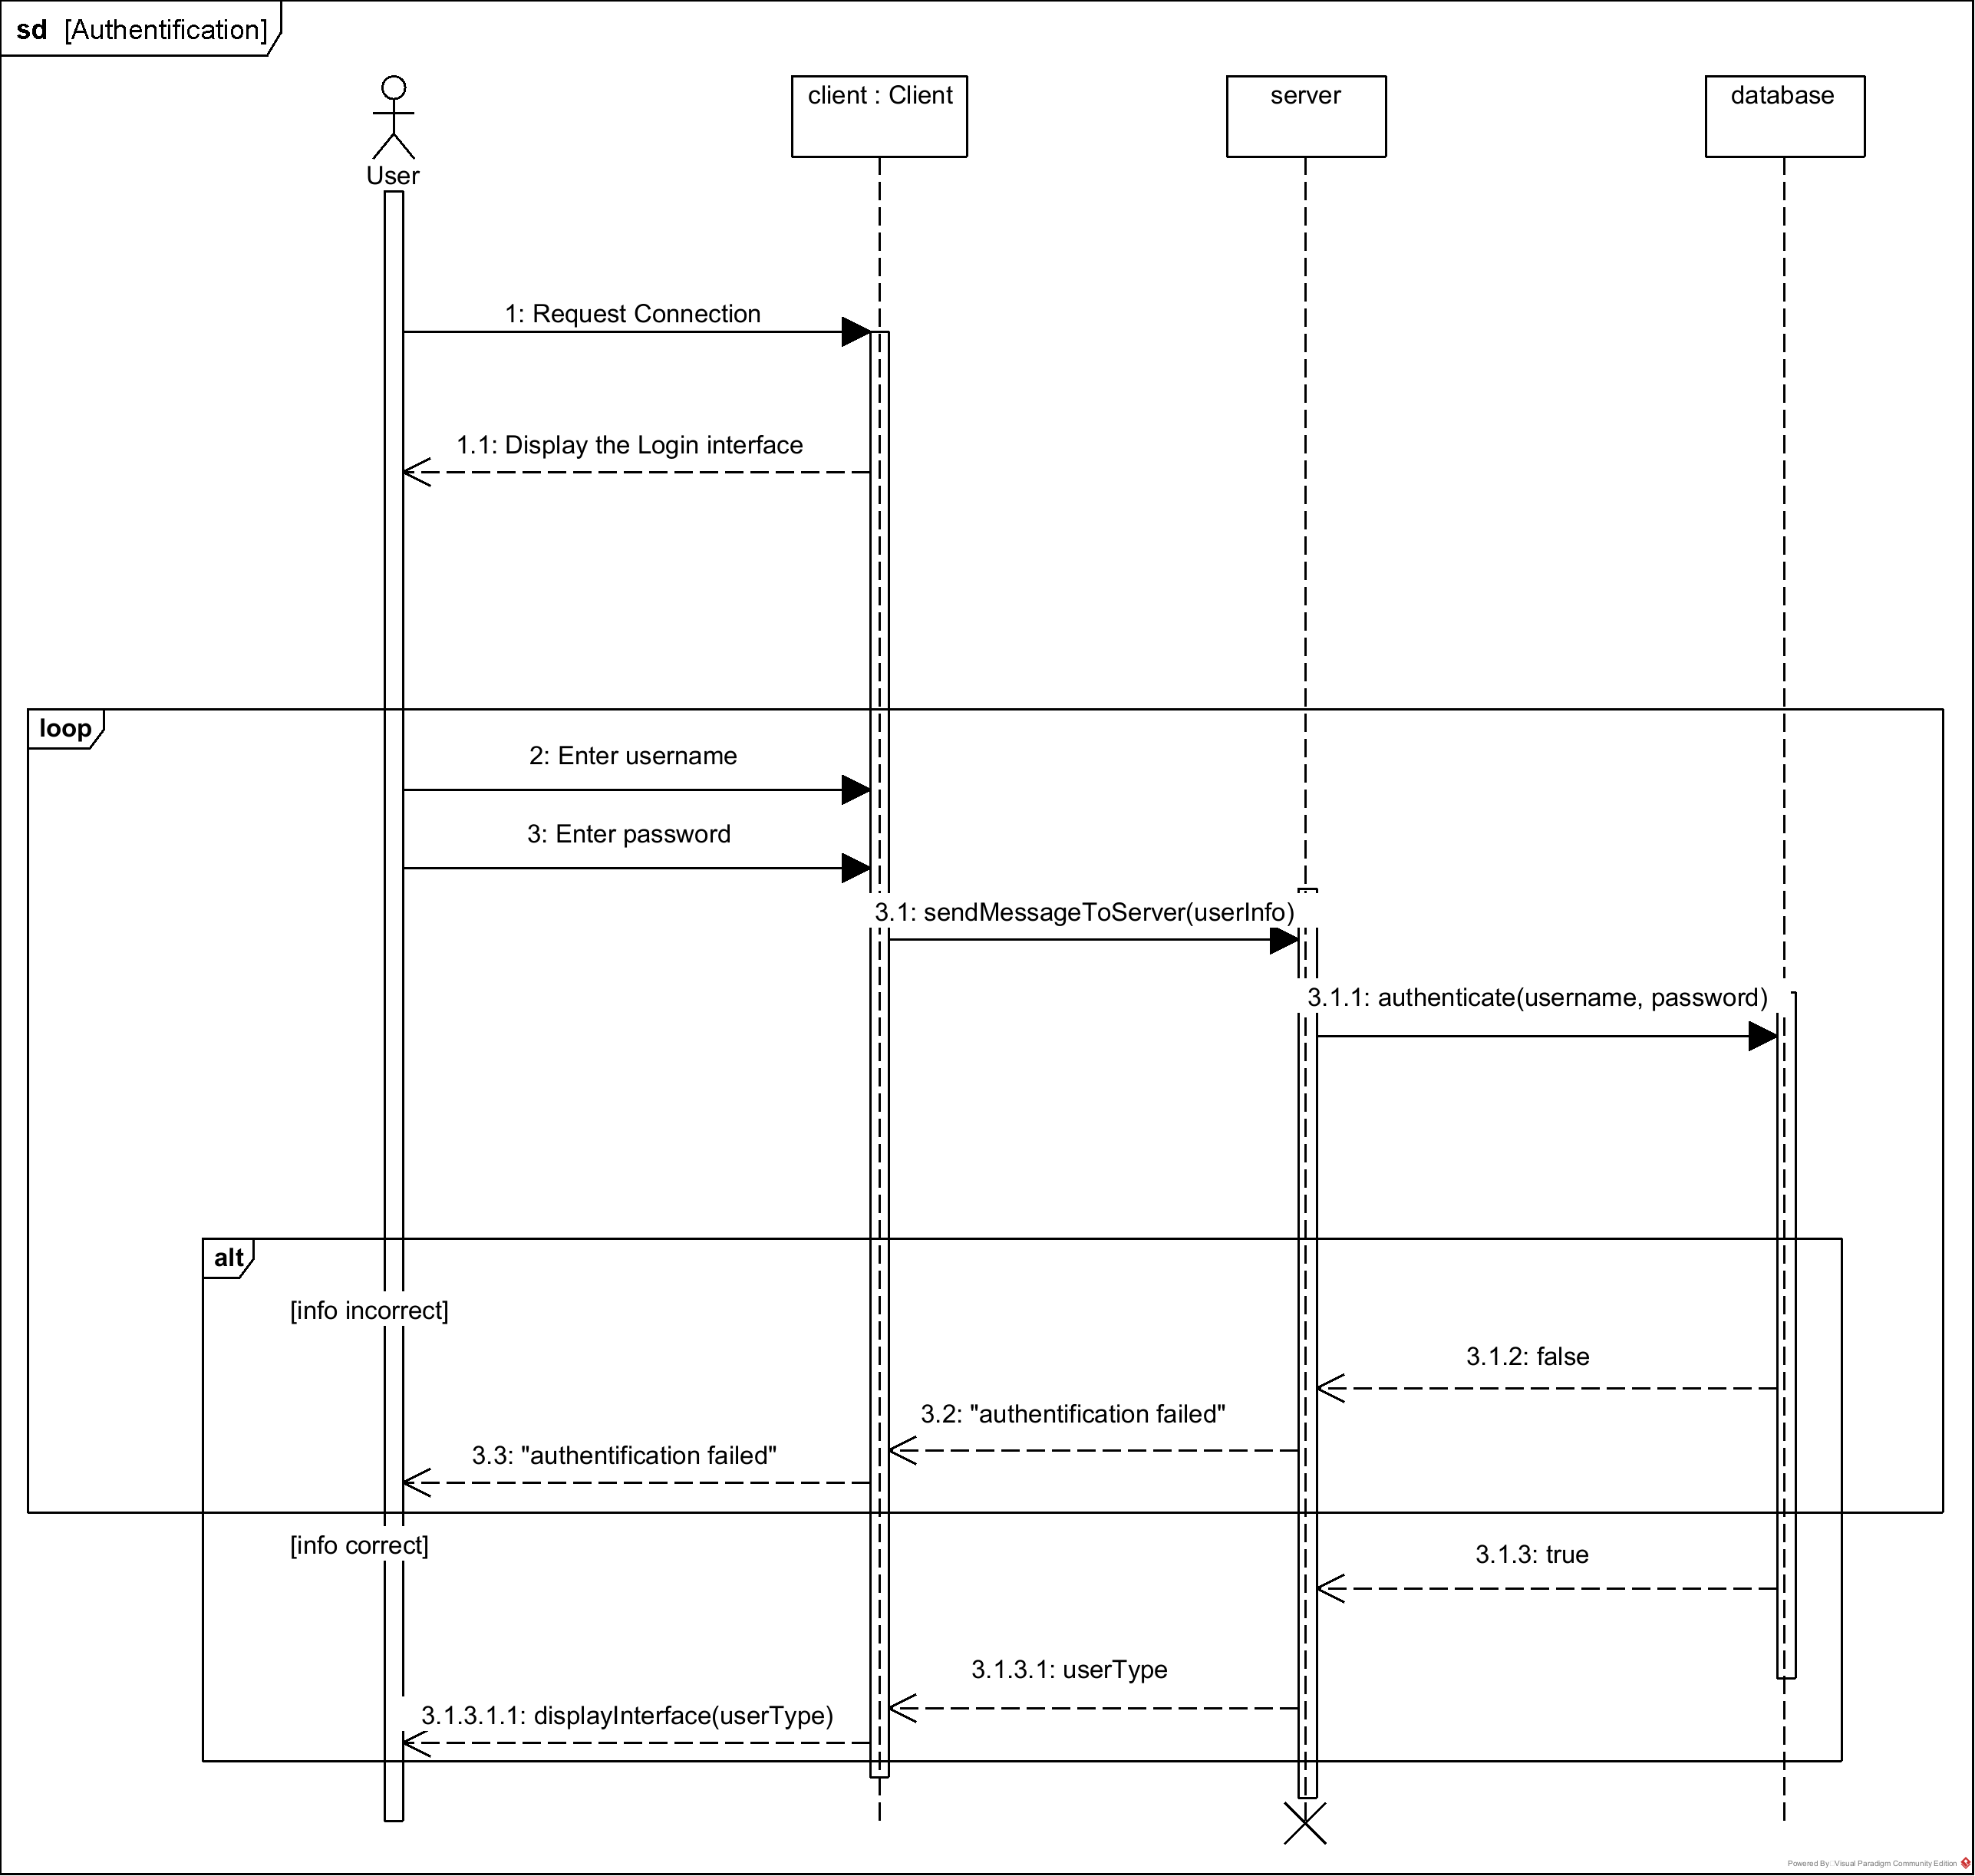
\includegraphics[width=451px]{media/sequence diagrams/Authentification.png}
    \captionof{figure}{Sequence Diagram for the Authentication}
\end{center}

\newpage
This Sequence Diagram showcases the sequence of interactions between the user and the system in order to search for an existing user.

\begin{center}
    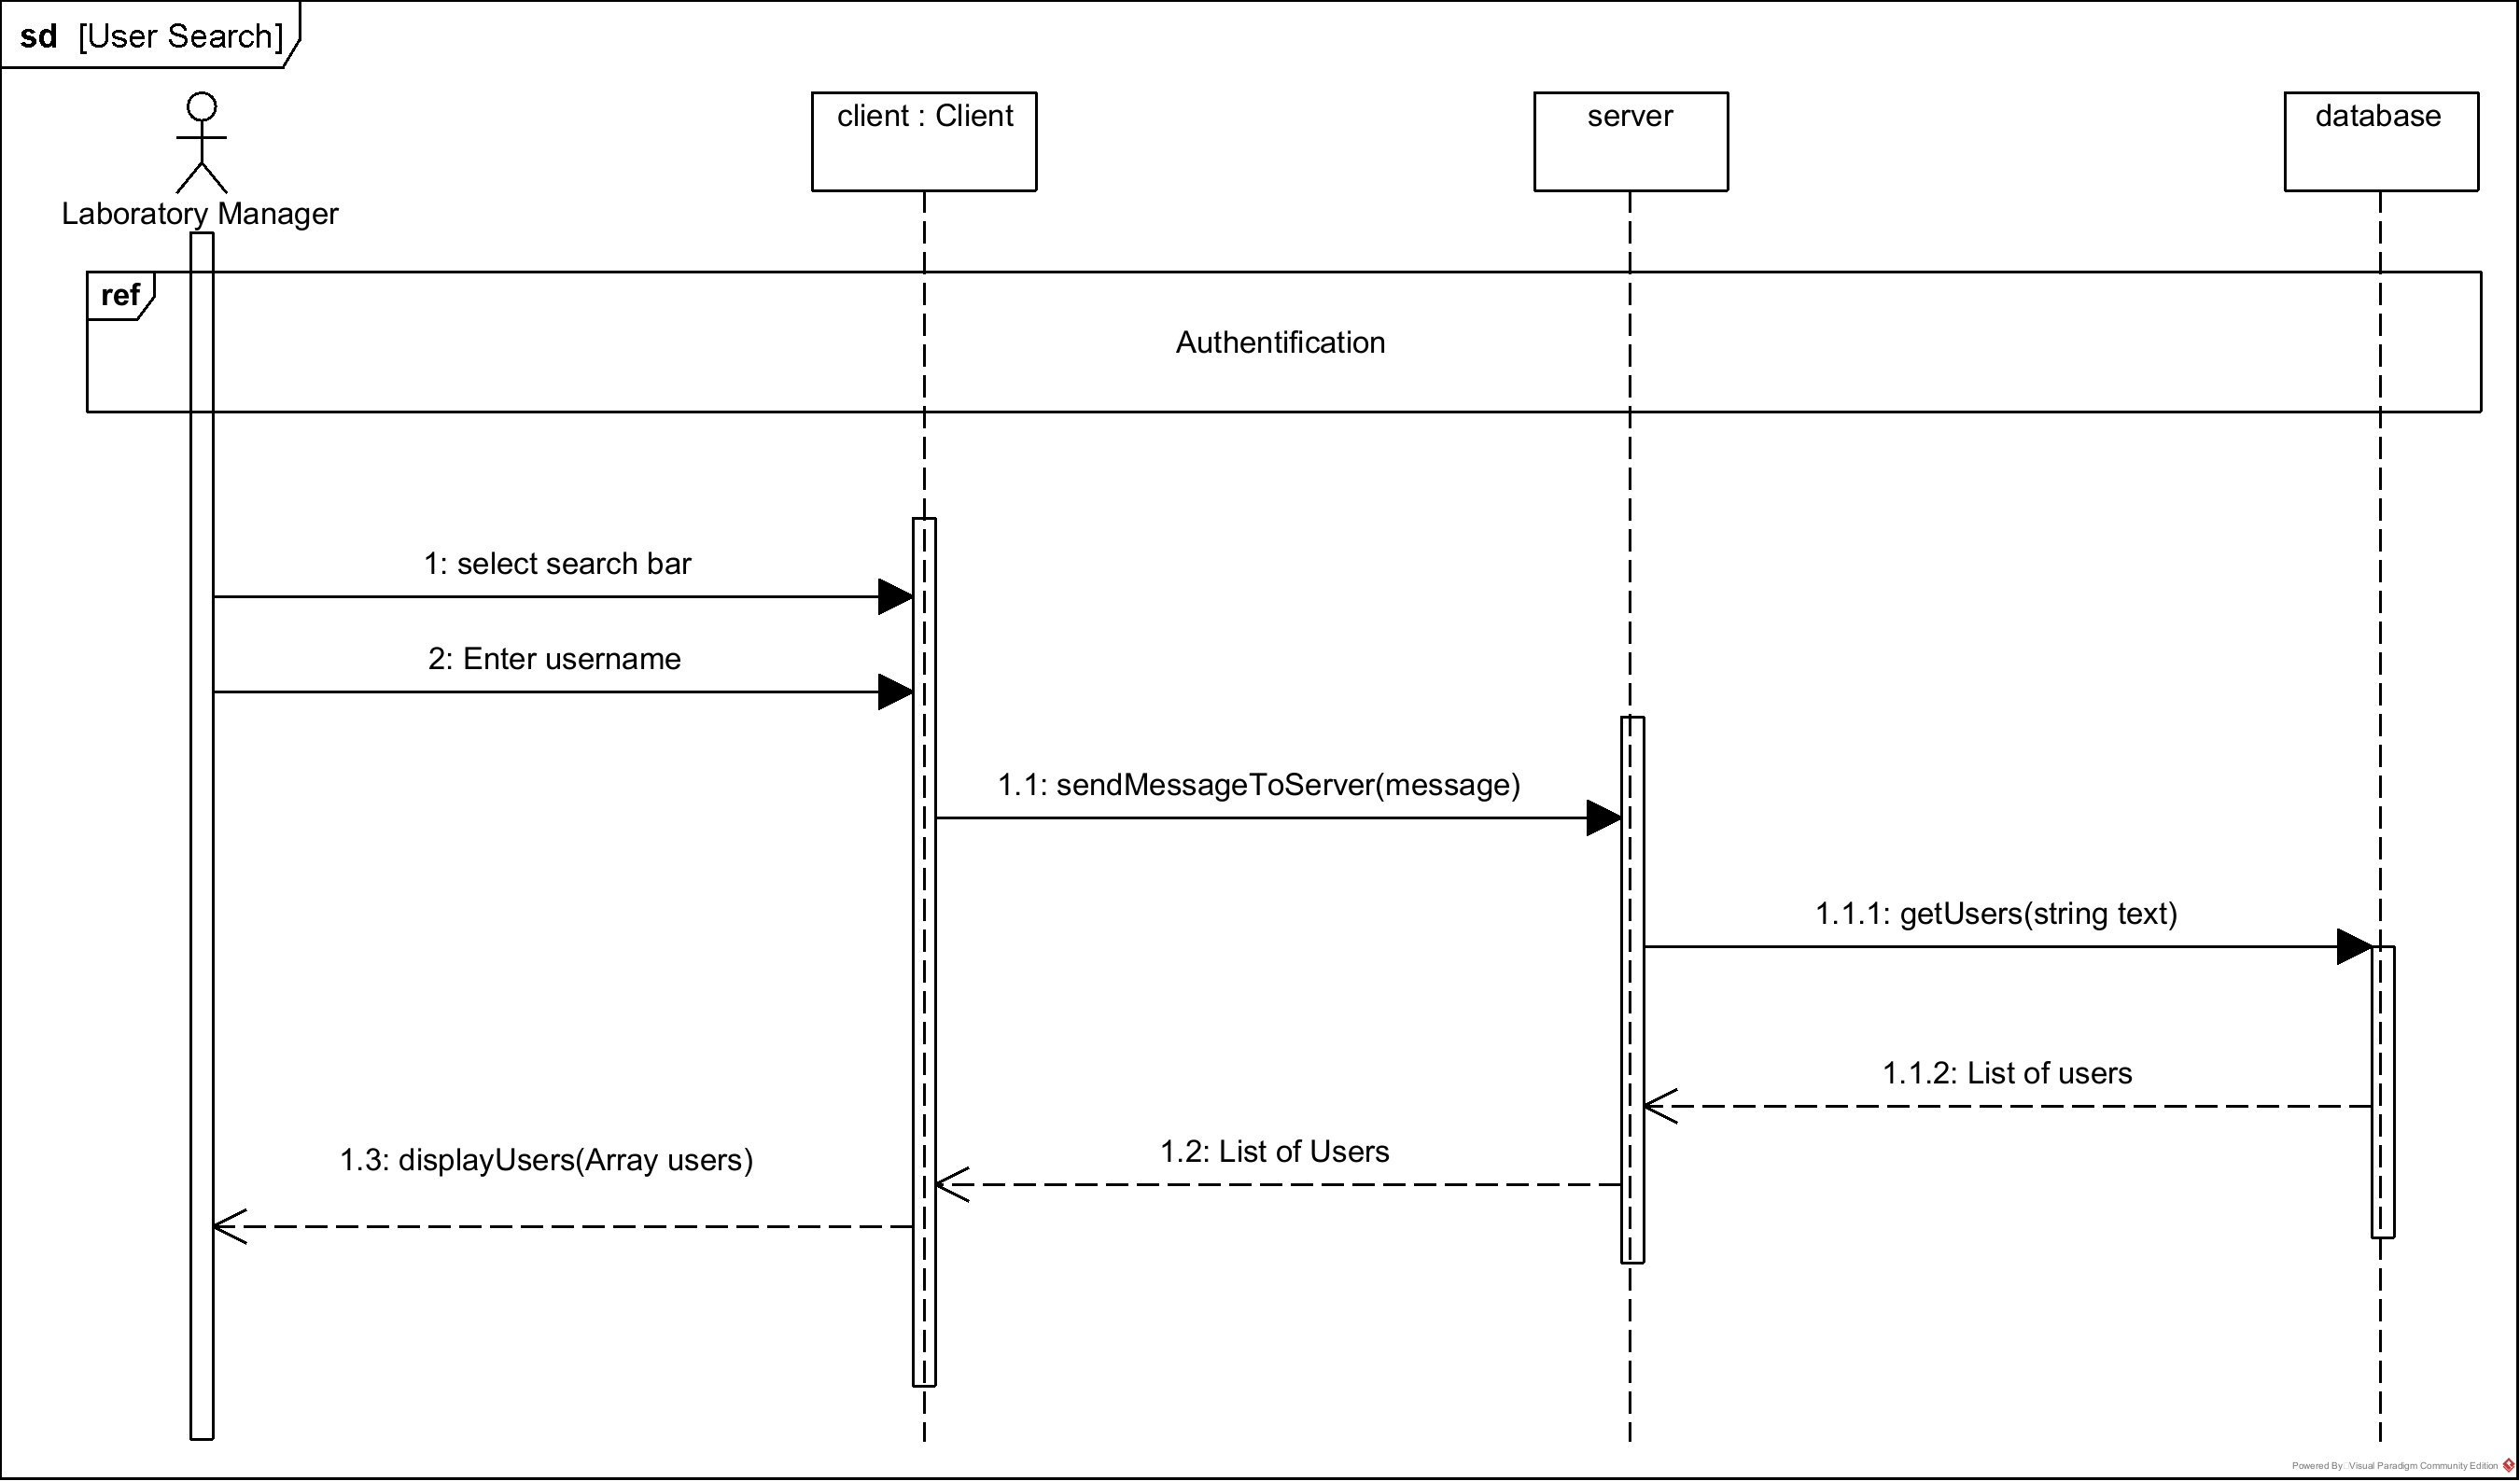
\includegraphics[width=451px]{media/sequence diagrams/User Search.png}
    \captionof{figure}{Sequence Diagram for searching a user}
\end{center}

\paragraph*{\textbf{Note: }} A similar version of the sequence diagram in [Figure 13] is used for the search of a patient, a sample, an equipment, and a test result.


\newpage
This Sequence Diagram explains the interactions between the user and the system components for adding a new user to the database.

\begin{center}
    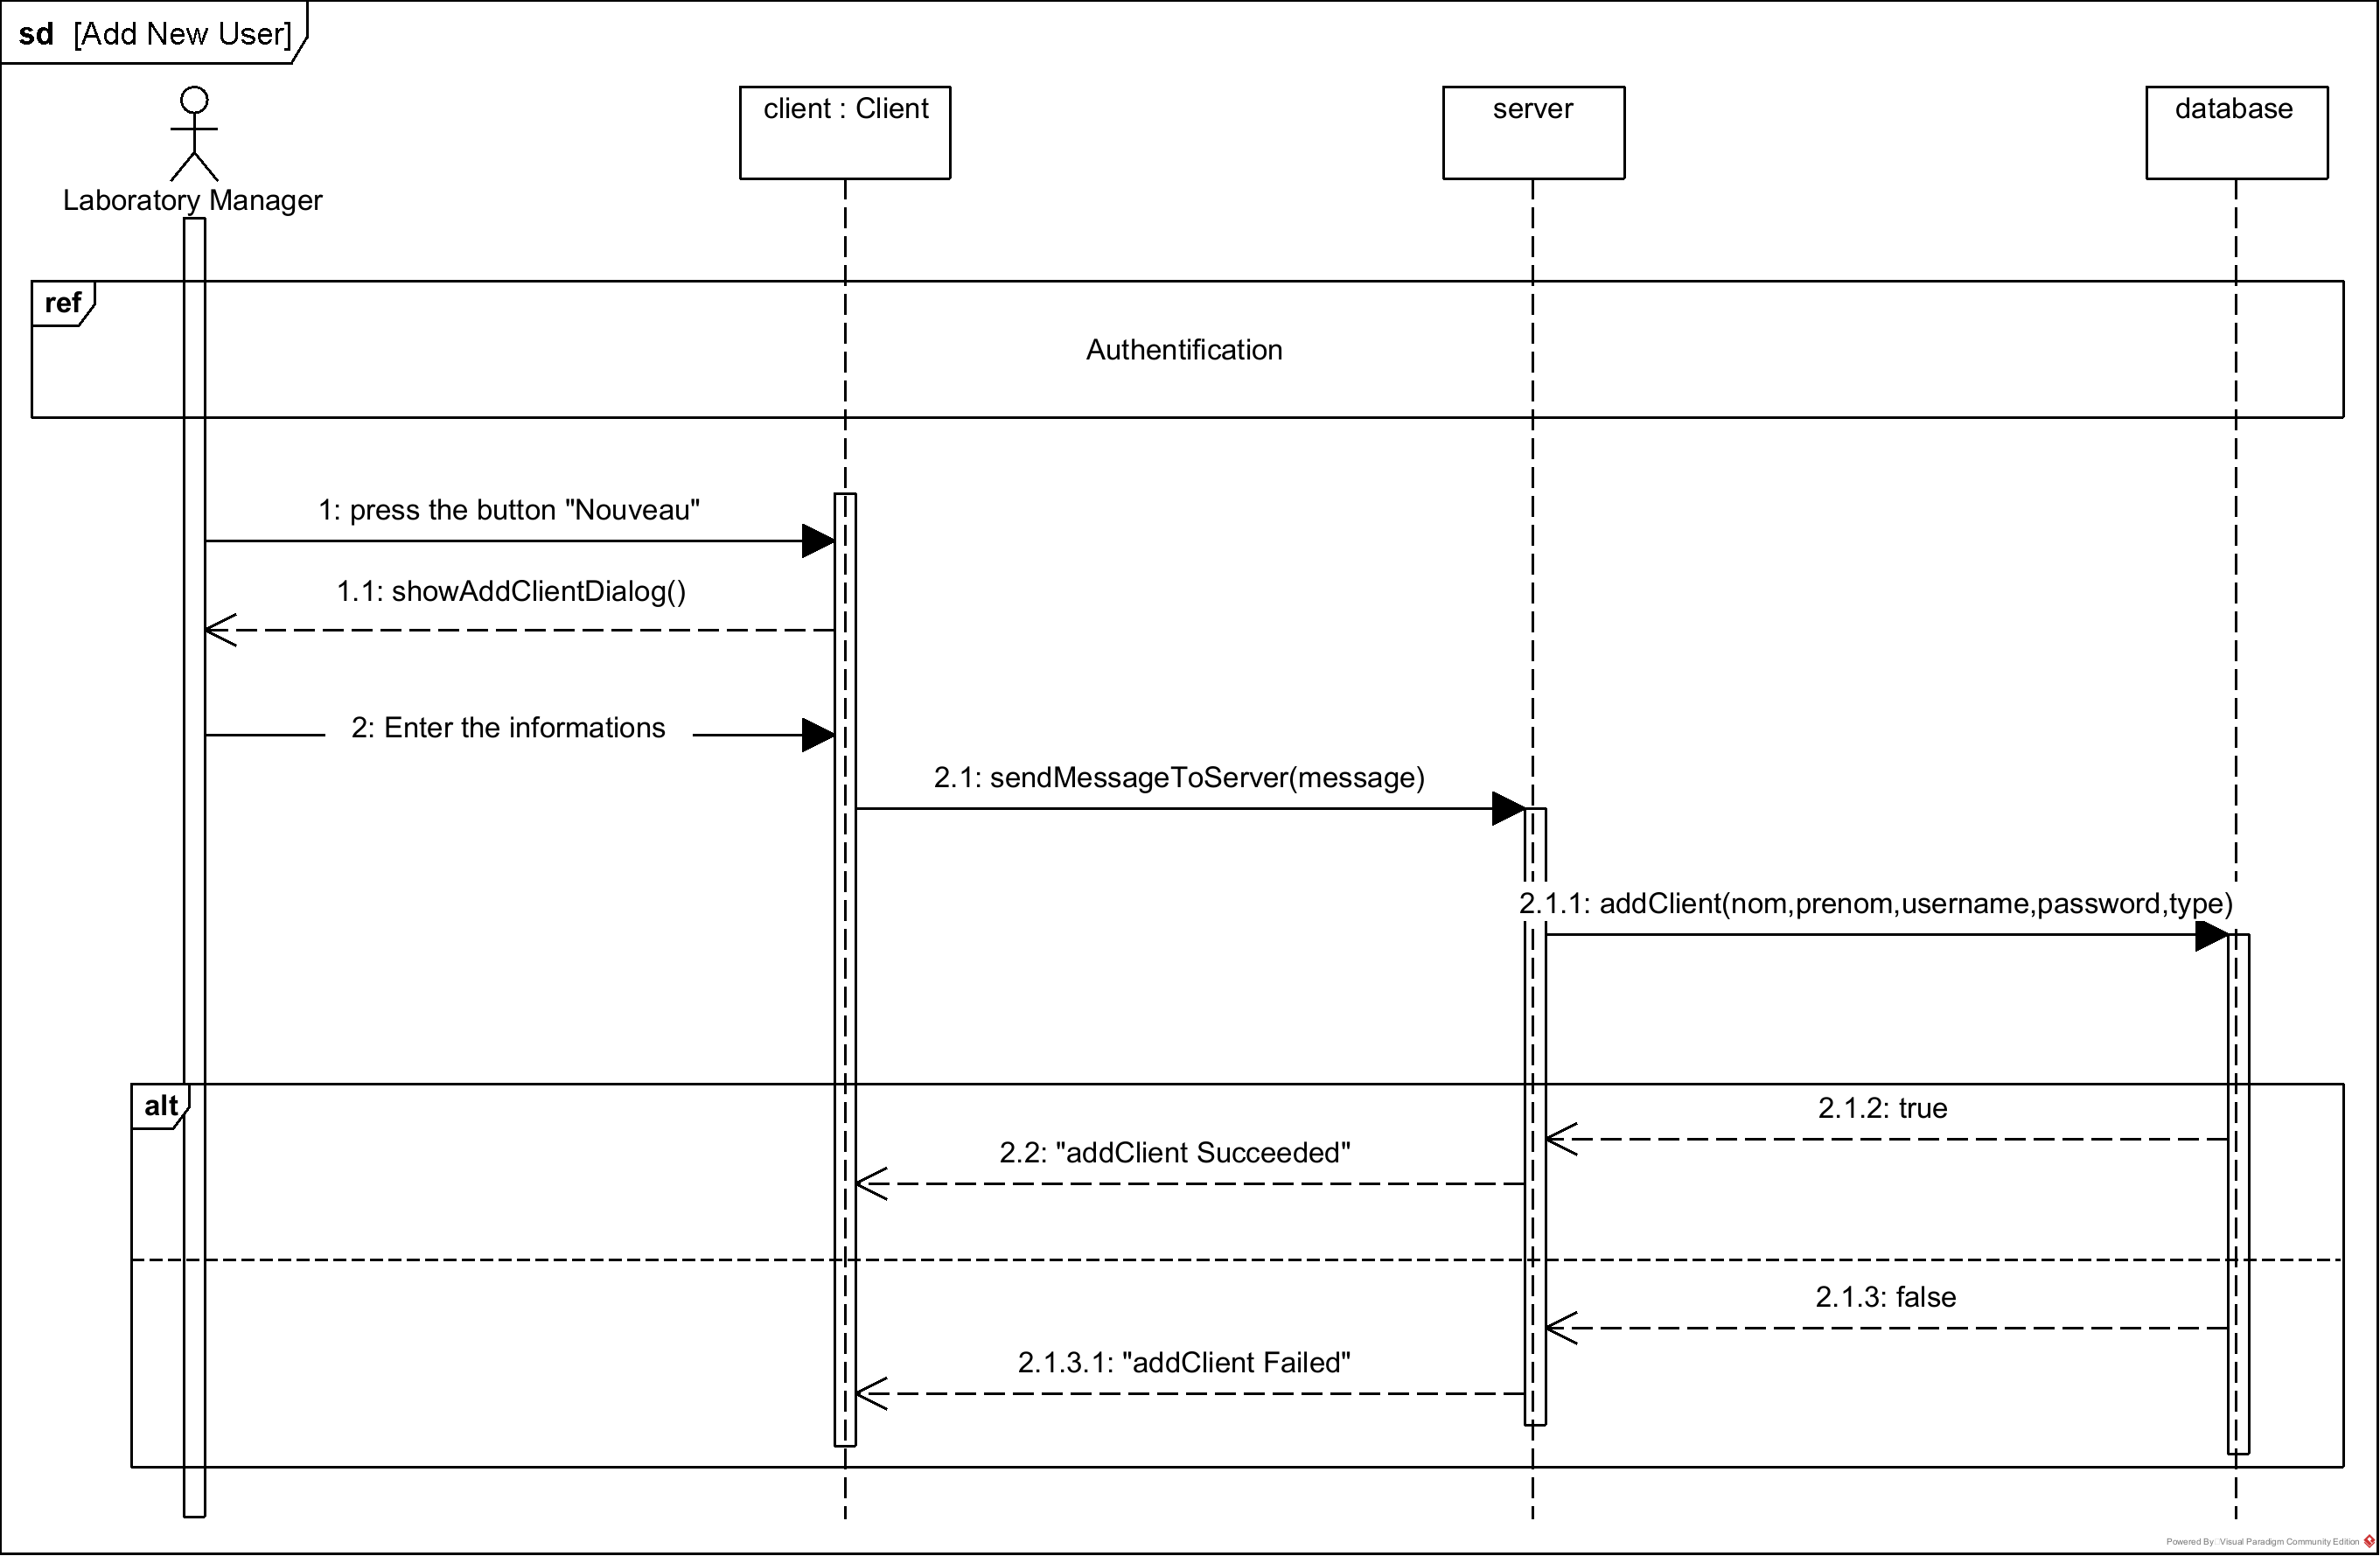
\includegraphics[width=451px]{media/sequence diagrams/Add New User.png}
    \captionof{figure}{Sequence Diagram for adding a user}
\end{center}

\paragraph*{\textbf{Note: }} A similar version of the sequence diagram in [Figure 14] is used for adding a patient, a sample request, an equipment, a payment or purchase.

\newpage
This Sequence Diagram represents the user-system interactions for modifying the information of an existing user.

\begin{center}
    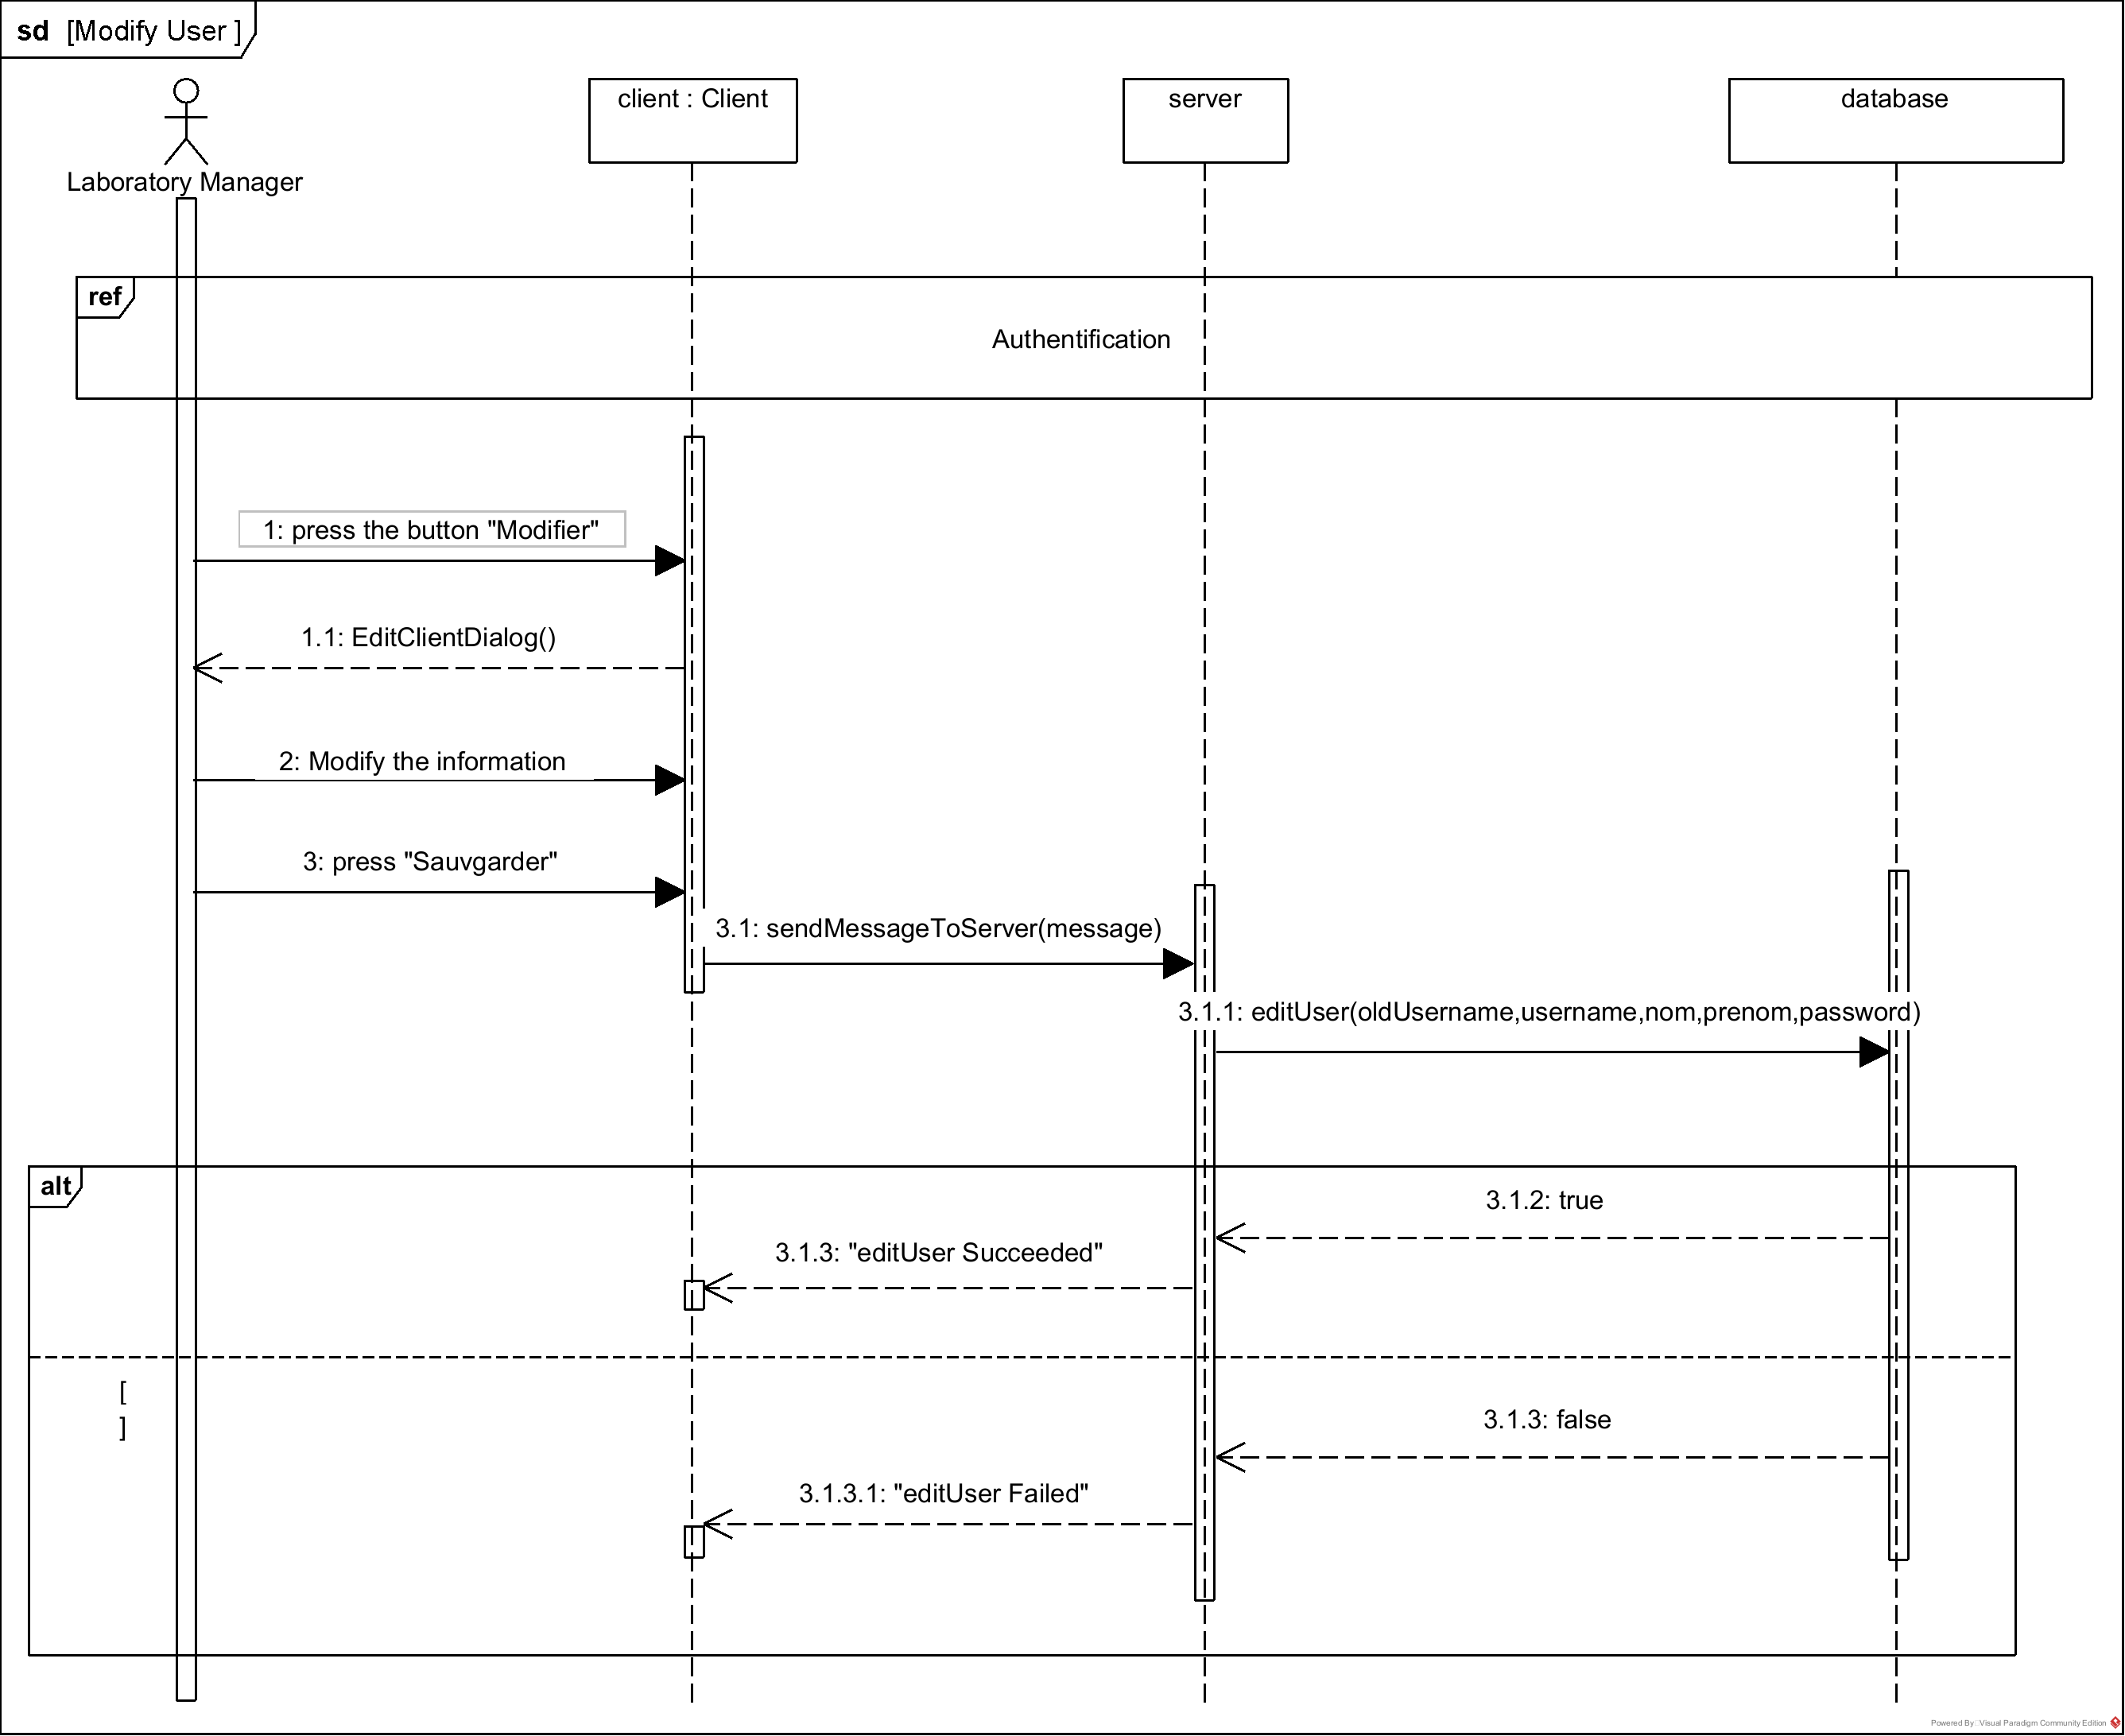
\includegraphics[width=451px]{media/sequence diagrams/Modify User.png}
    \captionof{figure}{Sequence Diagram for modifying a user}
\end{center}

\paragraph*{\textbf{Note: }} A similar version of the sequence diagram in [Figure 15] is used for modifying a patient, an equipment.

\newpage
This Sequence Diagram details the various interactions between the user and the system for deleting an existing user.

\begin{center}
    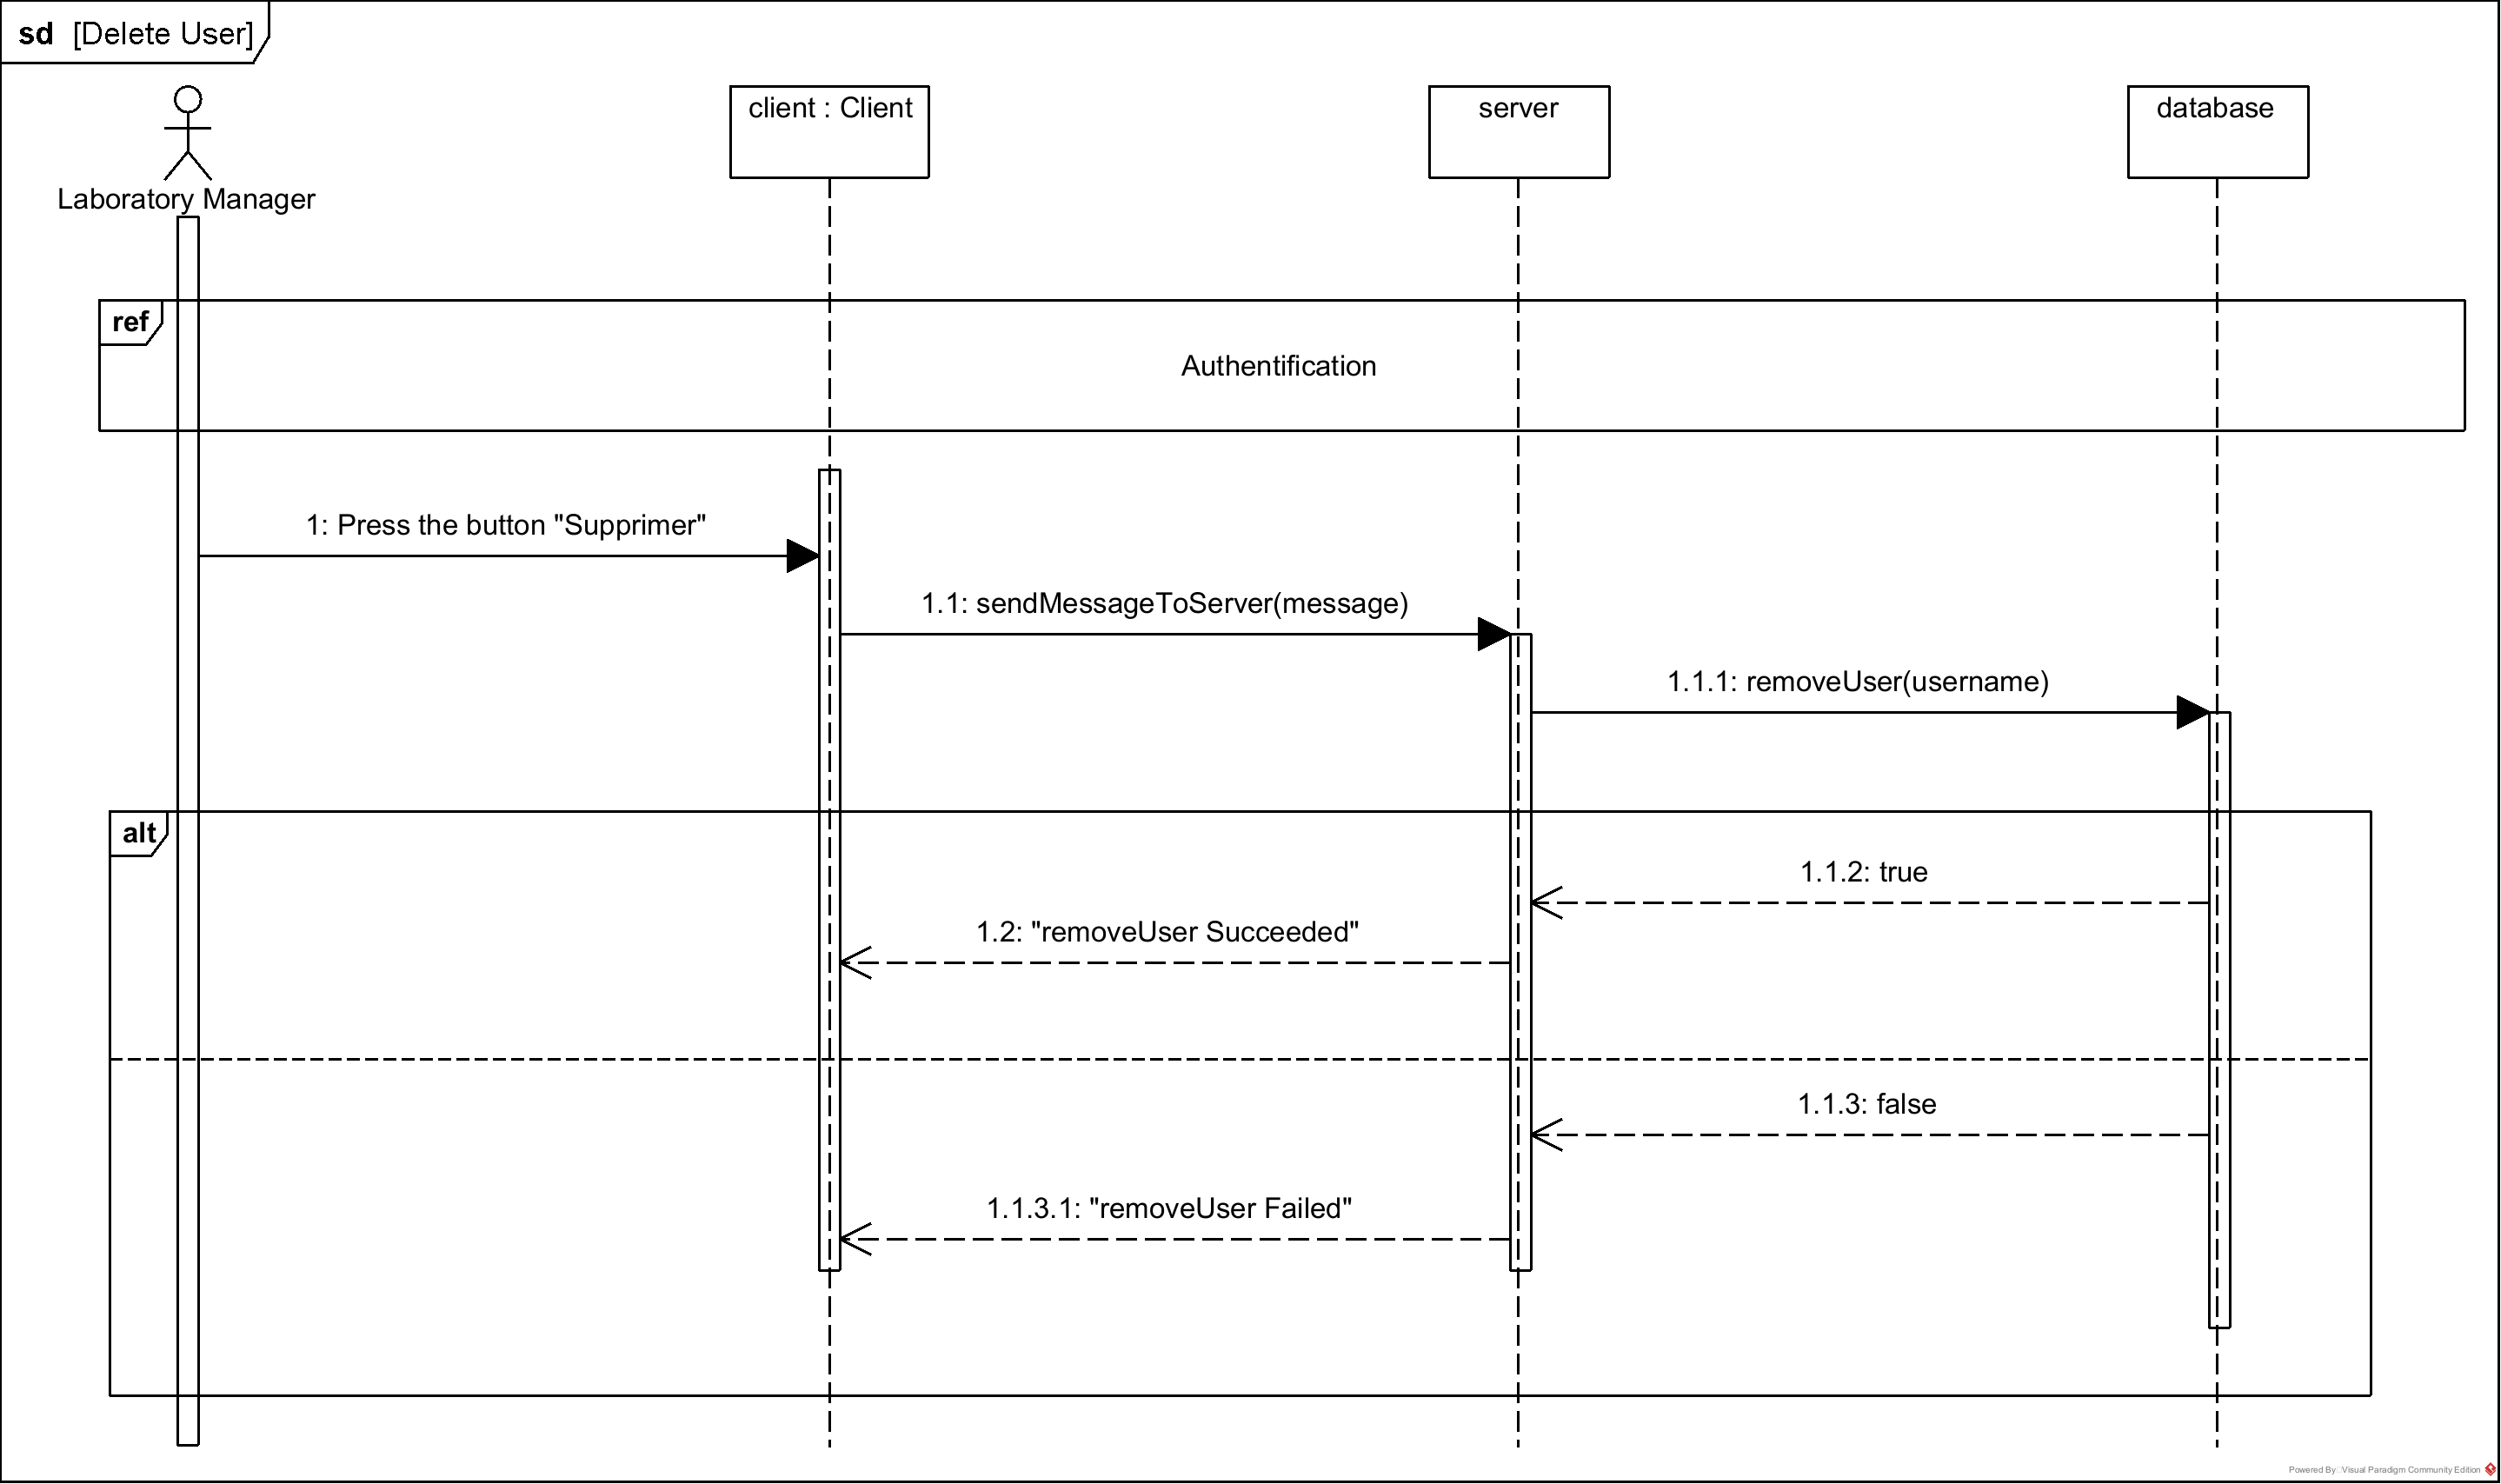
\includegraphics[width=451px]{media/sequence diagrams/Delete User.png}
    \captionof{figure}{Sequence Diagram for deleting a user}
\end{center}

\paragraph*{\textbf{Note: }} A similar version of the sequence diagram in [Figure 16] is used for deleting a patient, an equipment, a sample request.

\newpage
This Sequence Diagram details the various interactions between the user and the system for adding analysis test results.

\begin{center}
    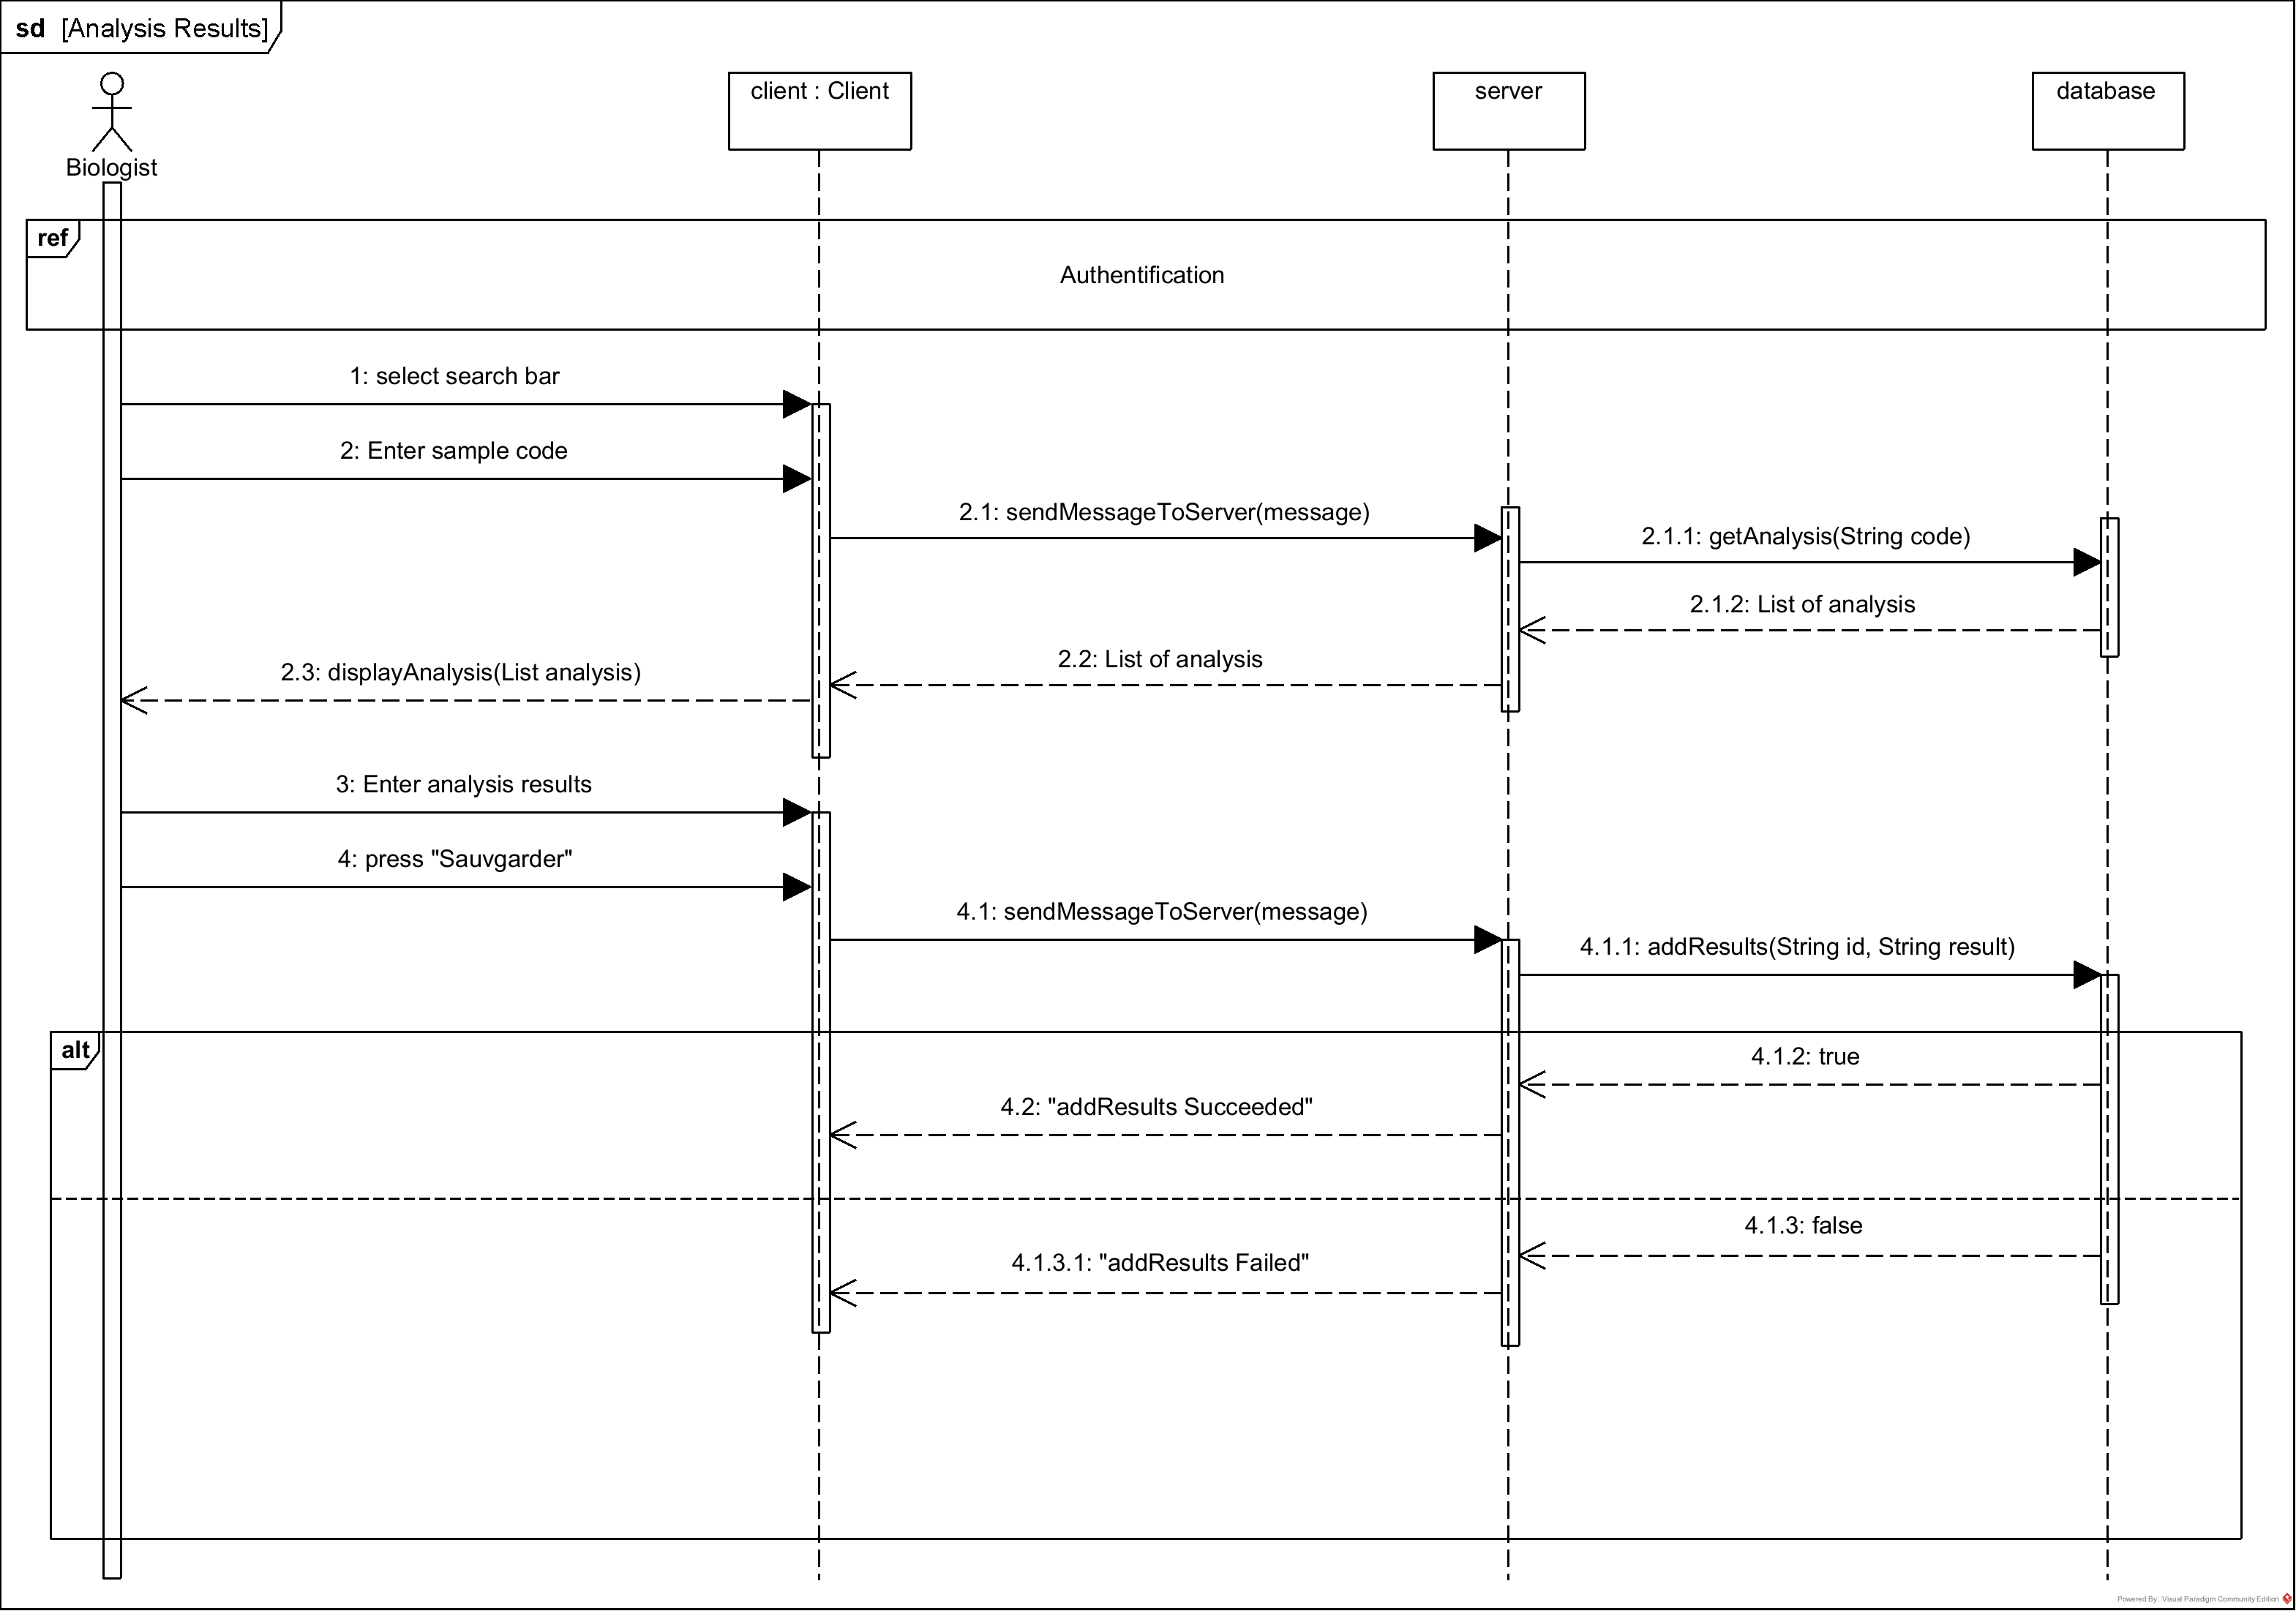
\includegraphics[width=451px]{media/sequence diagrams/Analysis Results.png}
    \captionof{figure}{Sequence Diagram for adding analysis results}
\end{center}

\paragraph*{\textbf{Note: }} A similar version of the sequence diagram in [Figure 17] is used for modifying an analysis results.

\newpage
This Sequence Diagram details the various interactions between the user and the system for the validation of analysis results.

\begin{center}
    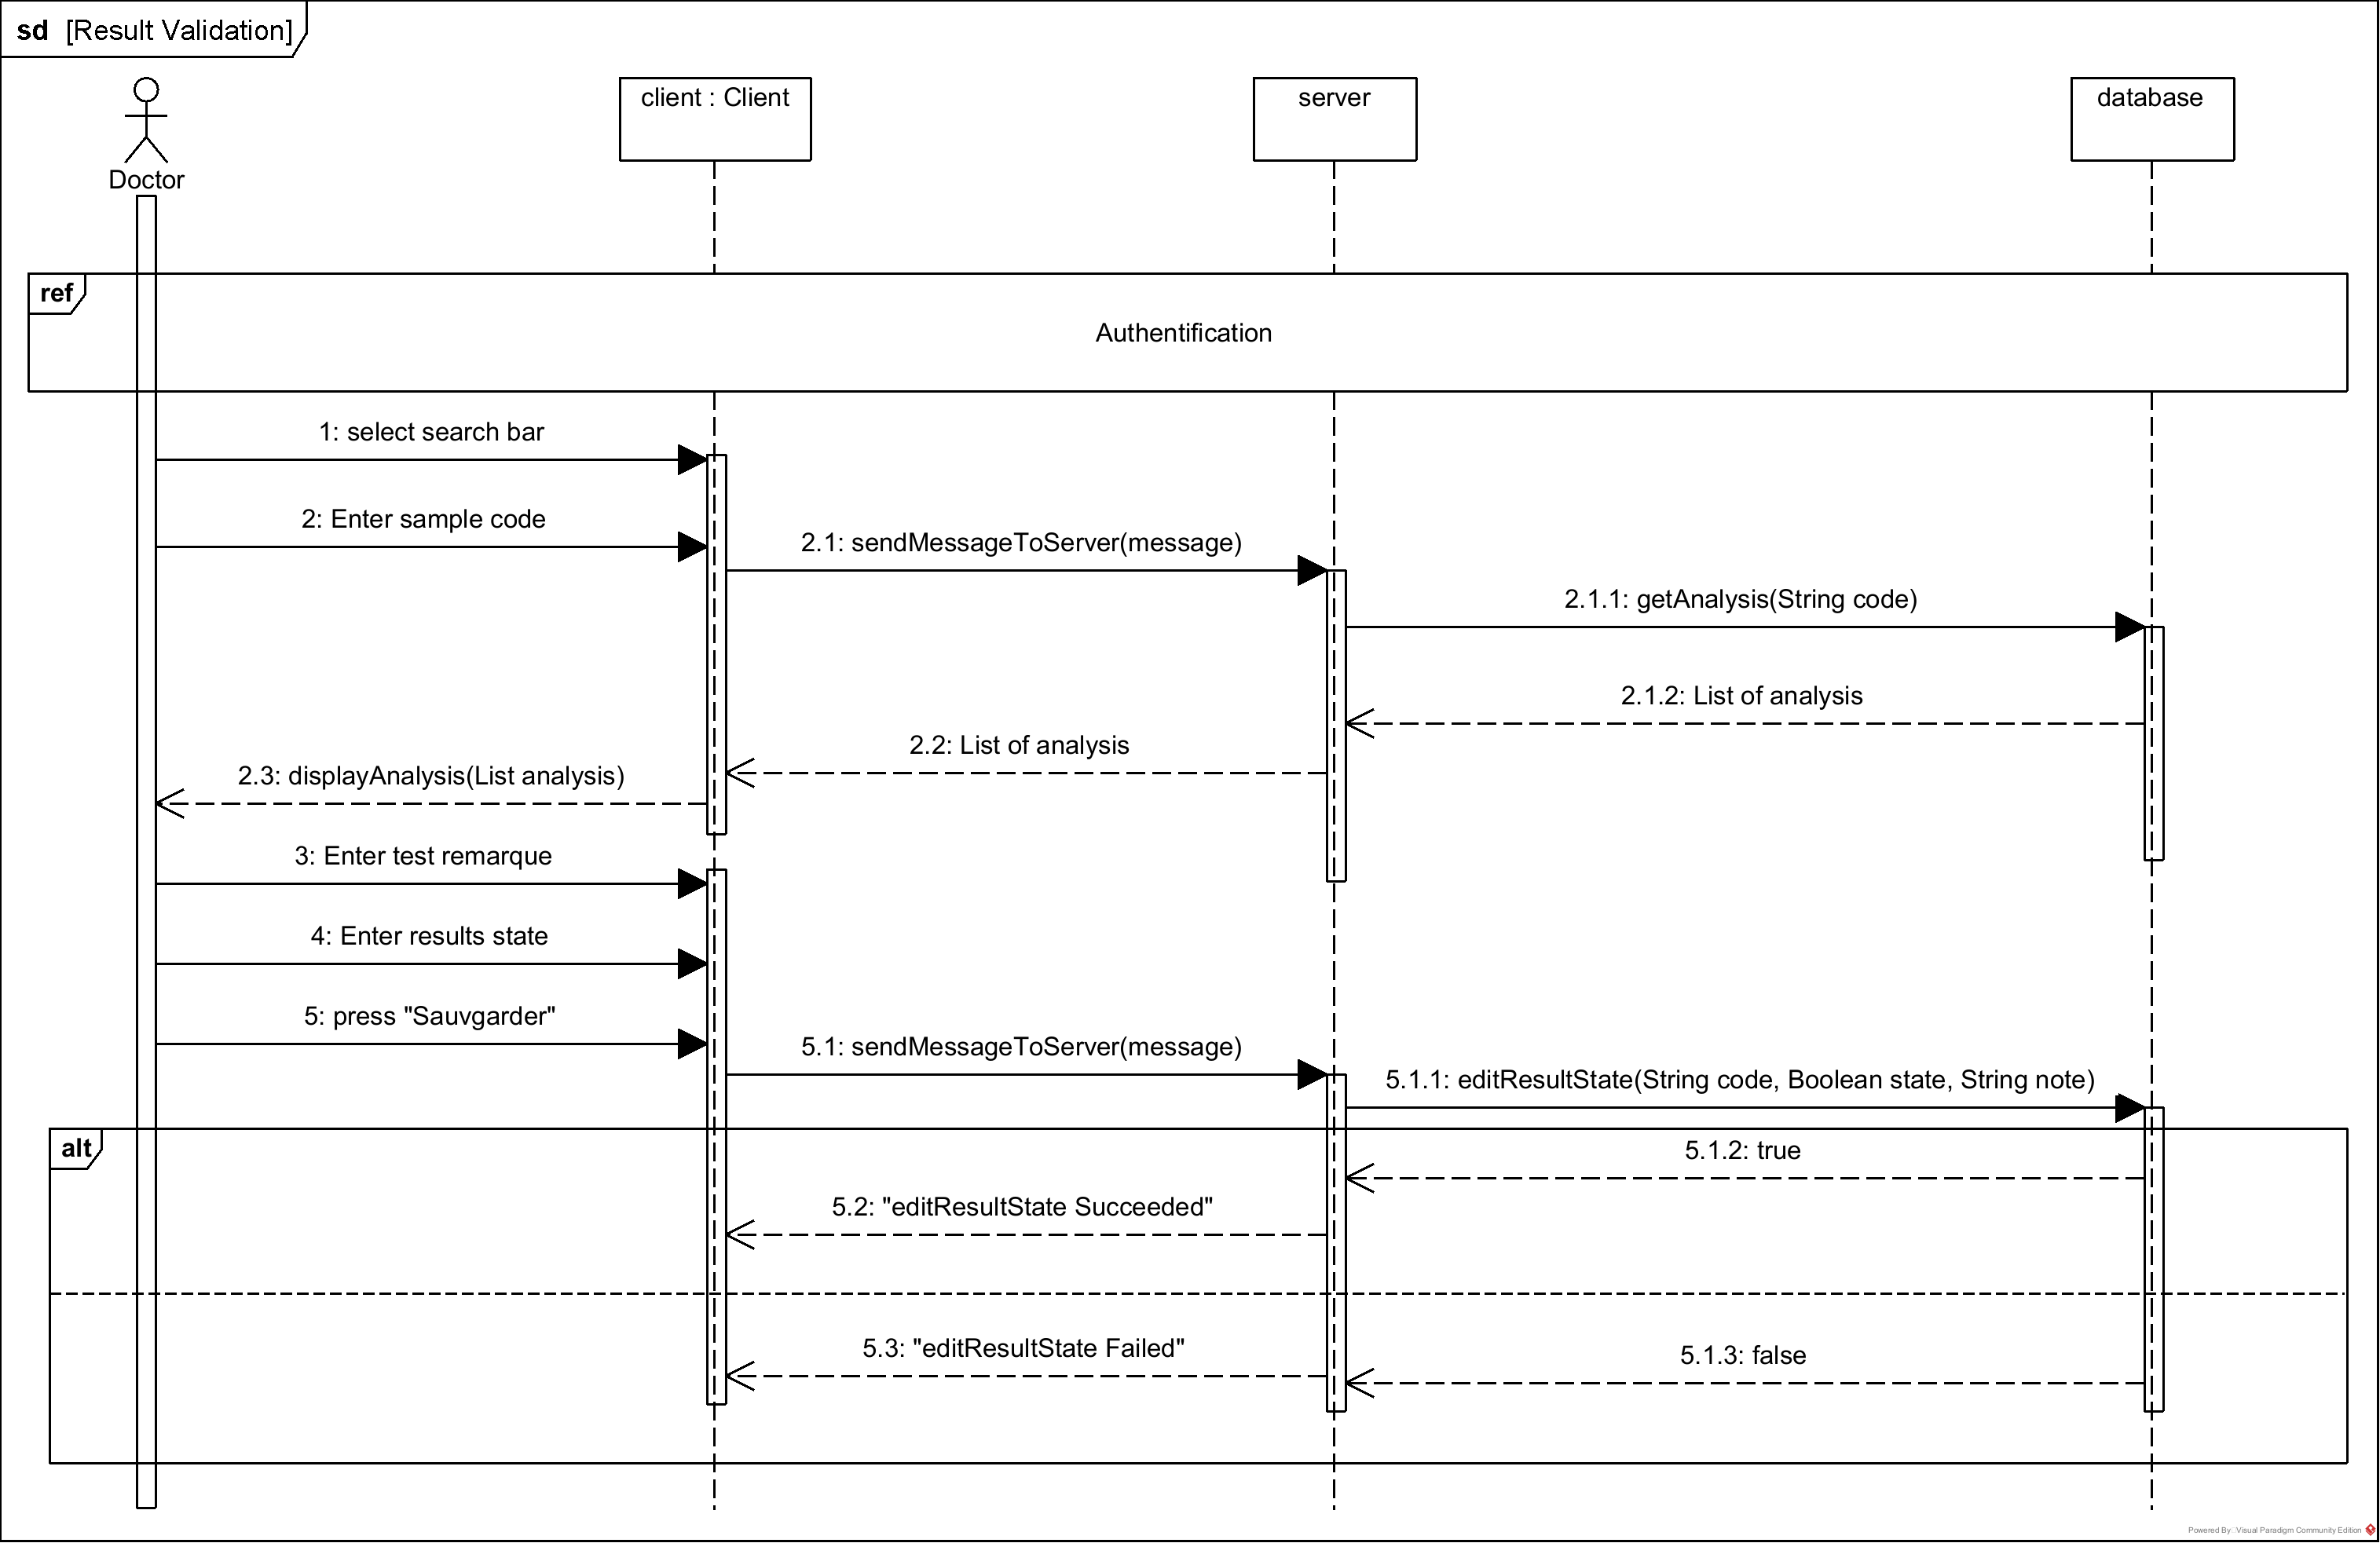
\includegraphics[width=451px]{media/sequence diagrams/result validation.png}
    \captionof{figure}{Sequence Diagram for analysis result validation}
\end{center}

\newpage
\subsubsection*{Class Diagram:}

\paragraph*{\textbf{Definition:} }

Class diagrams are a type of static structure diagram in UML that represent the structure of a system by showing the classes of the system, their attributes, methods, and relationships between them. They depict the static view of the system, focusing on the entities (classes) within the system and their relationships. Class diagrams are widely used in object-oriented analysis and design to model the structure of software systems.

\paragraph*{\textbf{Purpose: }}
\begin{itemize}
    \item Represents the state of the software.
    \item Represents the internal structure.
    \item Diagram evolution with the execution of the software (the creation, deletion, and modification (relation, object)).

\end{itemize}
\paragraph*{\textbf{Diagram Elements: }}
\vspace{0.3cm}
\begin{center}
    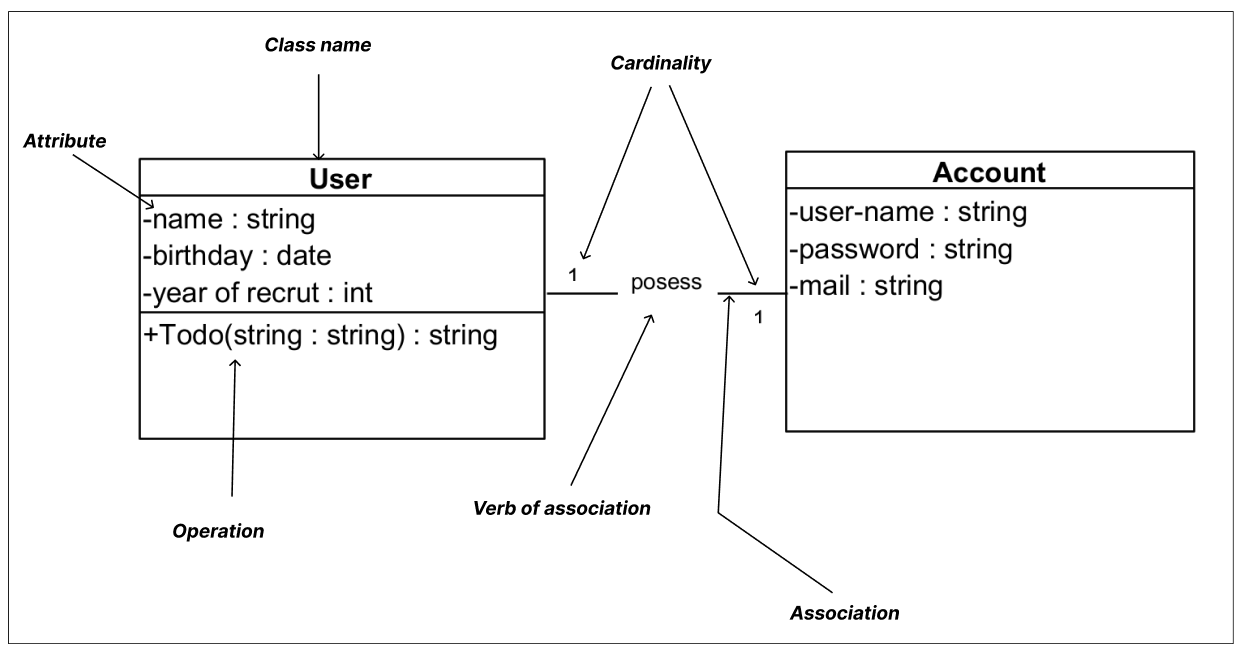
\includegraphics[width=451px]{media/class_elements.png}
    \captionof{figure}{Class Diagram Elements}
\end{center}
\vspace{1cm}
\noindent Here is our Class Diagram:
\newpage
This diagram shows us the detailed class tables that are needed in our application.

\begin{center}
    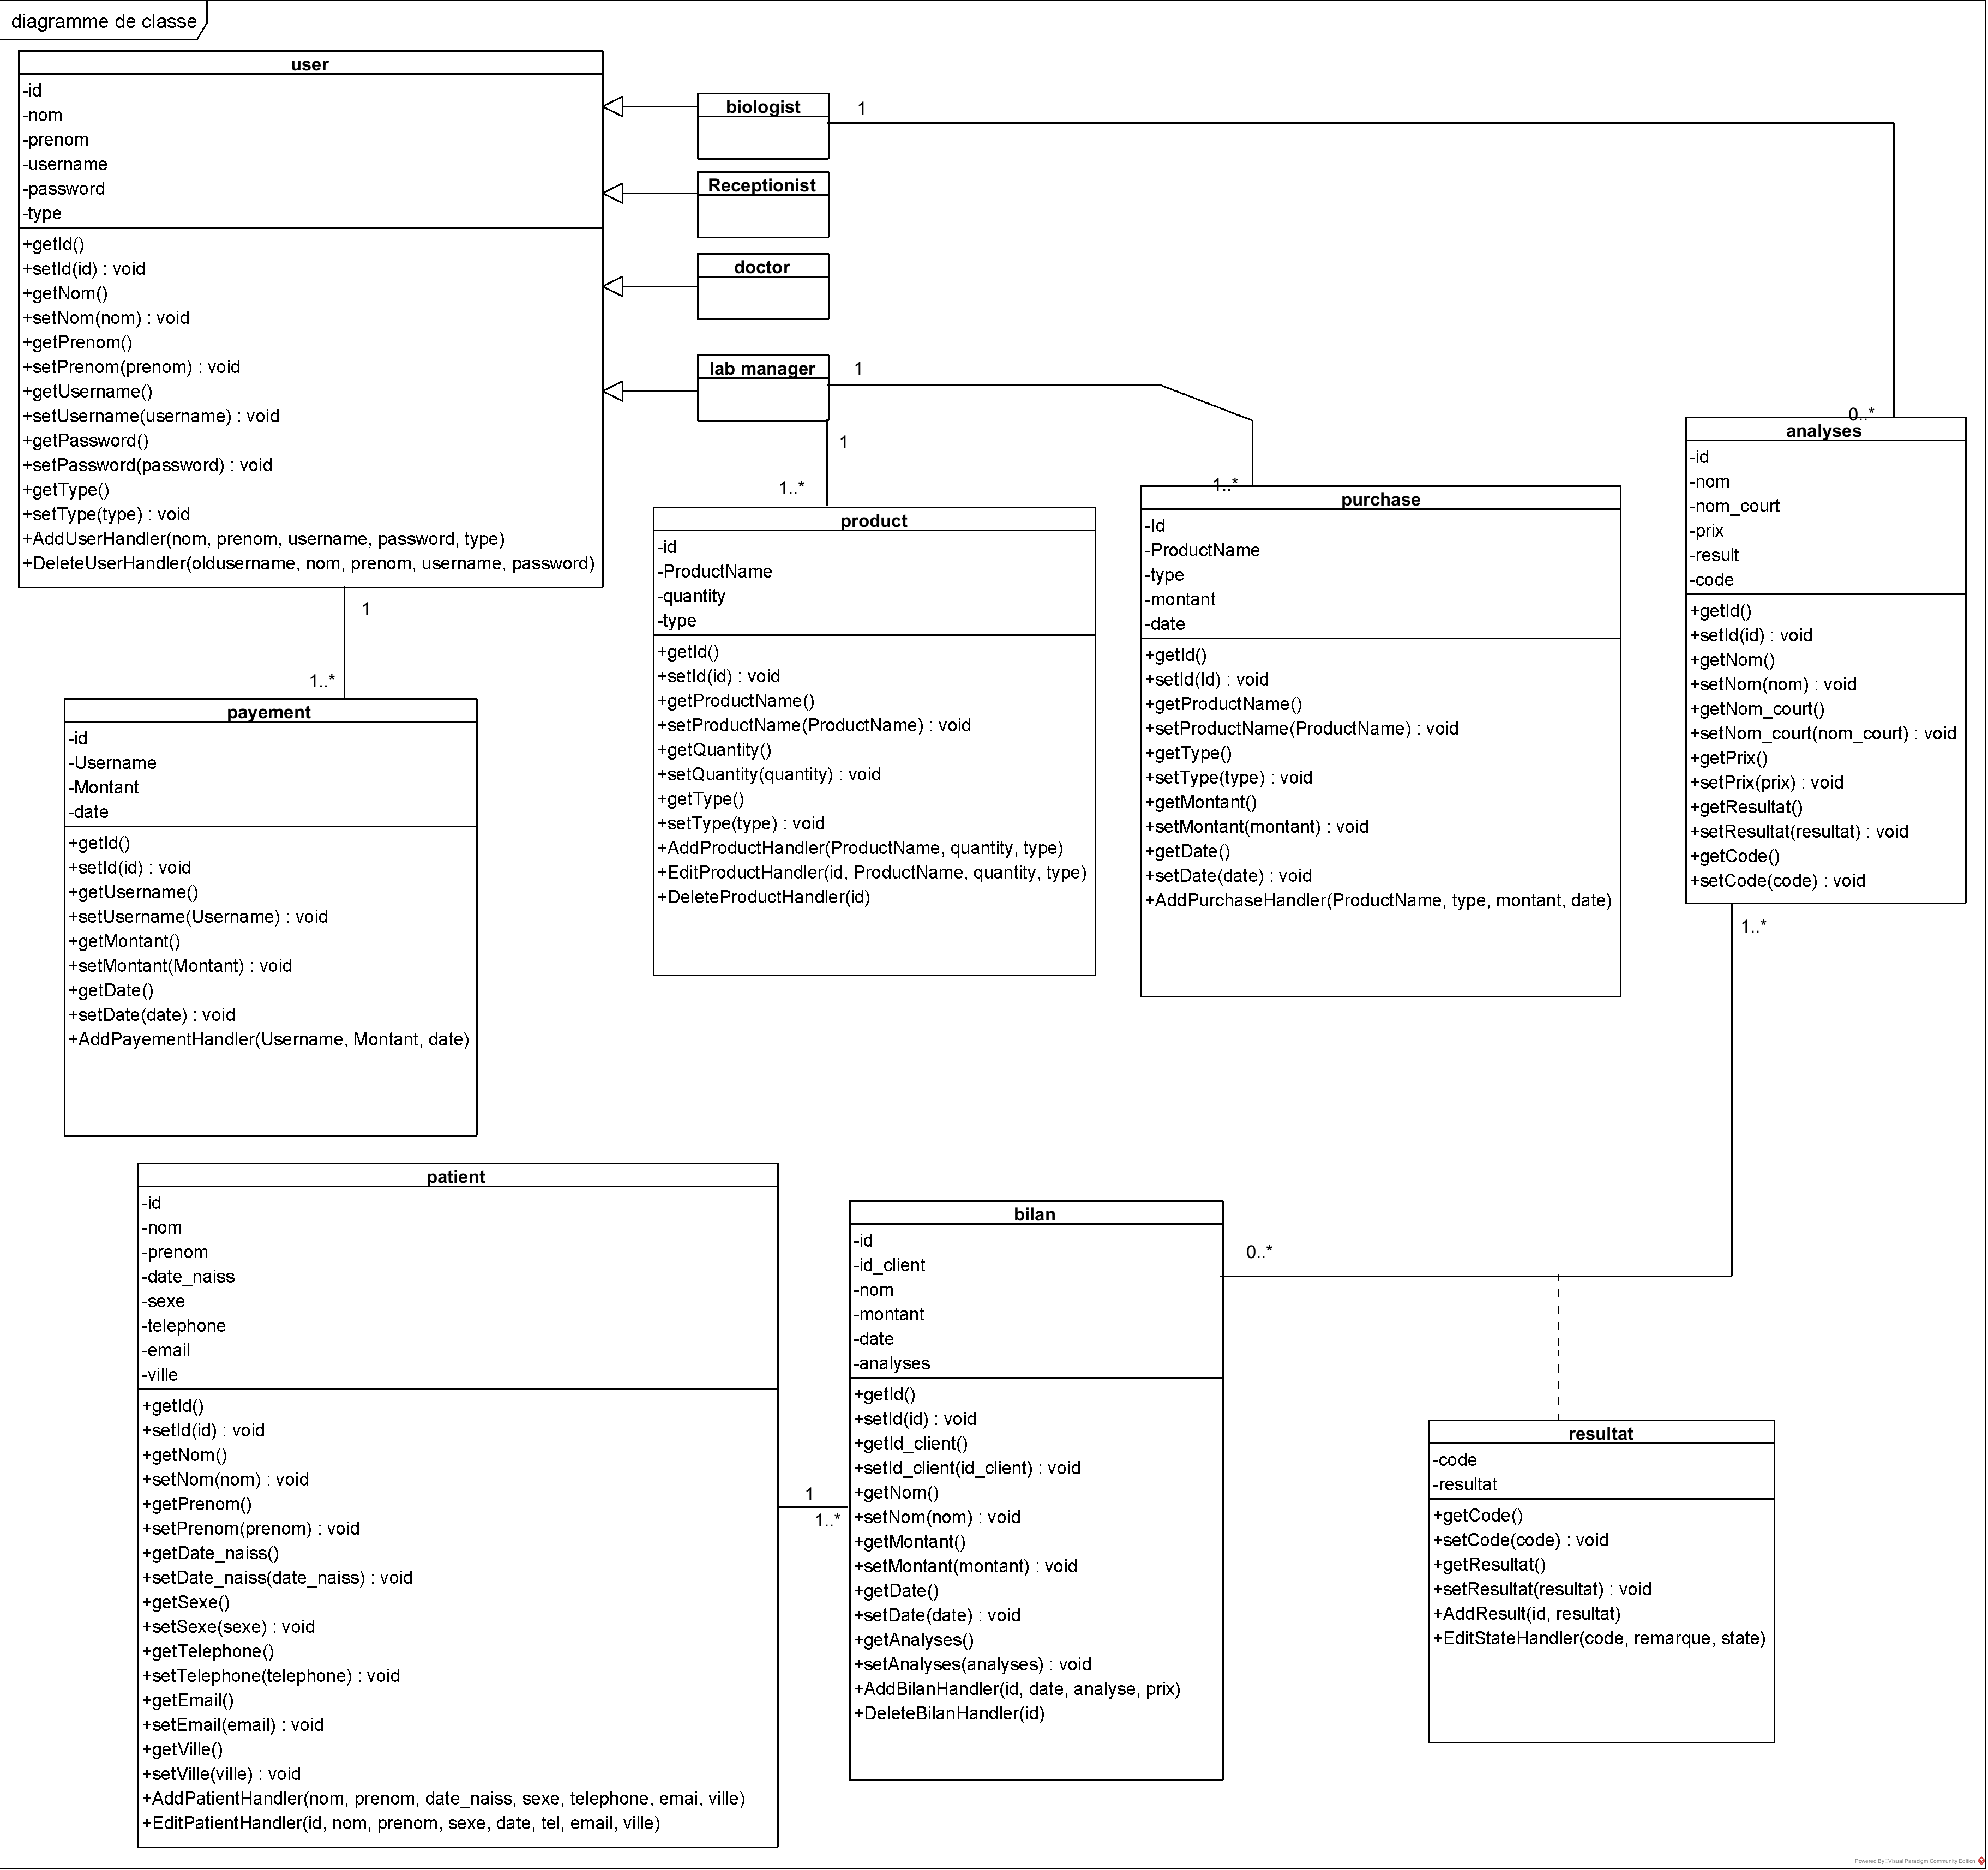
\includegraphics[width=451px]{media/class diagrams/app class diagram.png}
    \captionof{figure}{Detailed Class Diagram for our application}
\end{center}

\newpage

\subsubsection*{Entity Relationship Diagram:}

\paragraph*{\textbf{Definition:}}

An Entity-Relationship (ER) diagram is a type of data model that describes the logical structure of a database. It shows the relationships between entities and their attributes. ER diagrams are widely used in database design and are an essential tool for software developers, database administrators, and data analysts.

\paragraph*{\textbf{Purpose:}}
\begin{itemize}
    \item Visualize the structure of a database.
    \item Identify the entities and their relationships.
    \item Understand the flow of data in a system.
    \item Design a database schema.
\end{itemize}

\paragraph*{\textbf{Diagram Elements:}}
\vspace{0.3cm}
\begin{center}
    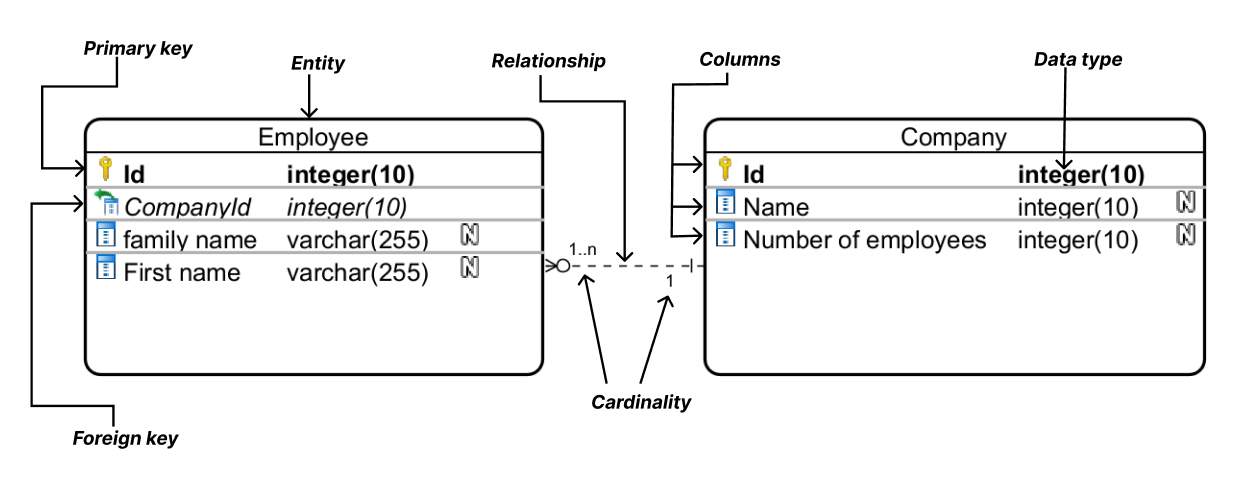
\includegraphics[width=451px]{media/entity_relationship_elements.png}
    \captionof{figure}{Entity Relationship Diagram Elements}
\end{center}
\vspace{1.5cm}
\noindent Here is our Entity Relationship Diagram:

\newpage
This Entity Relationship diagram represents the database tables that are used in our application.

\begin{center}
    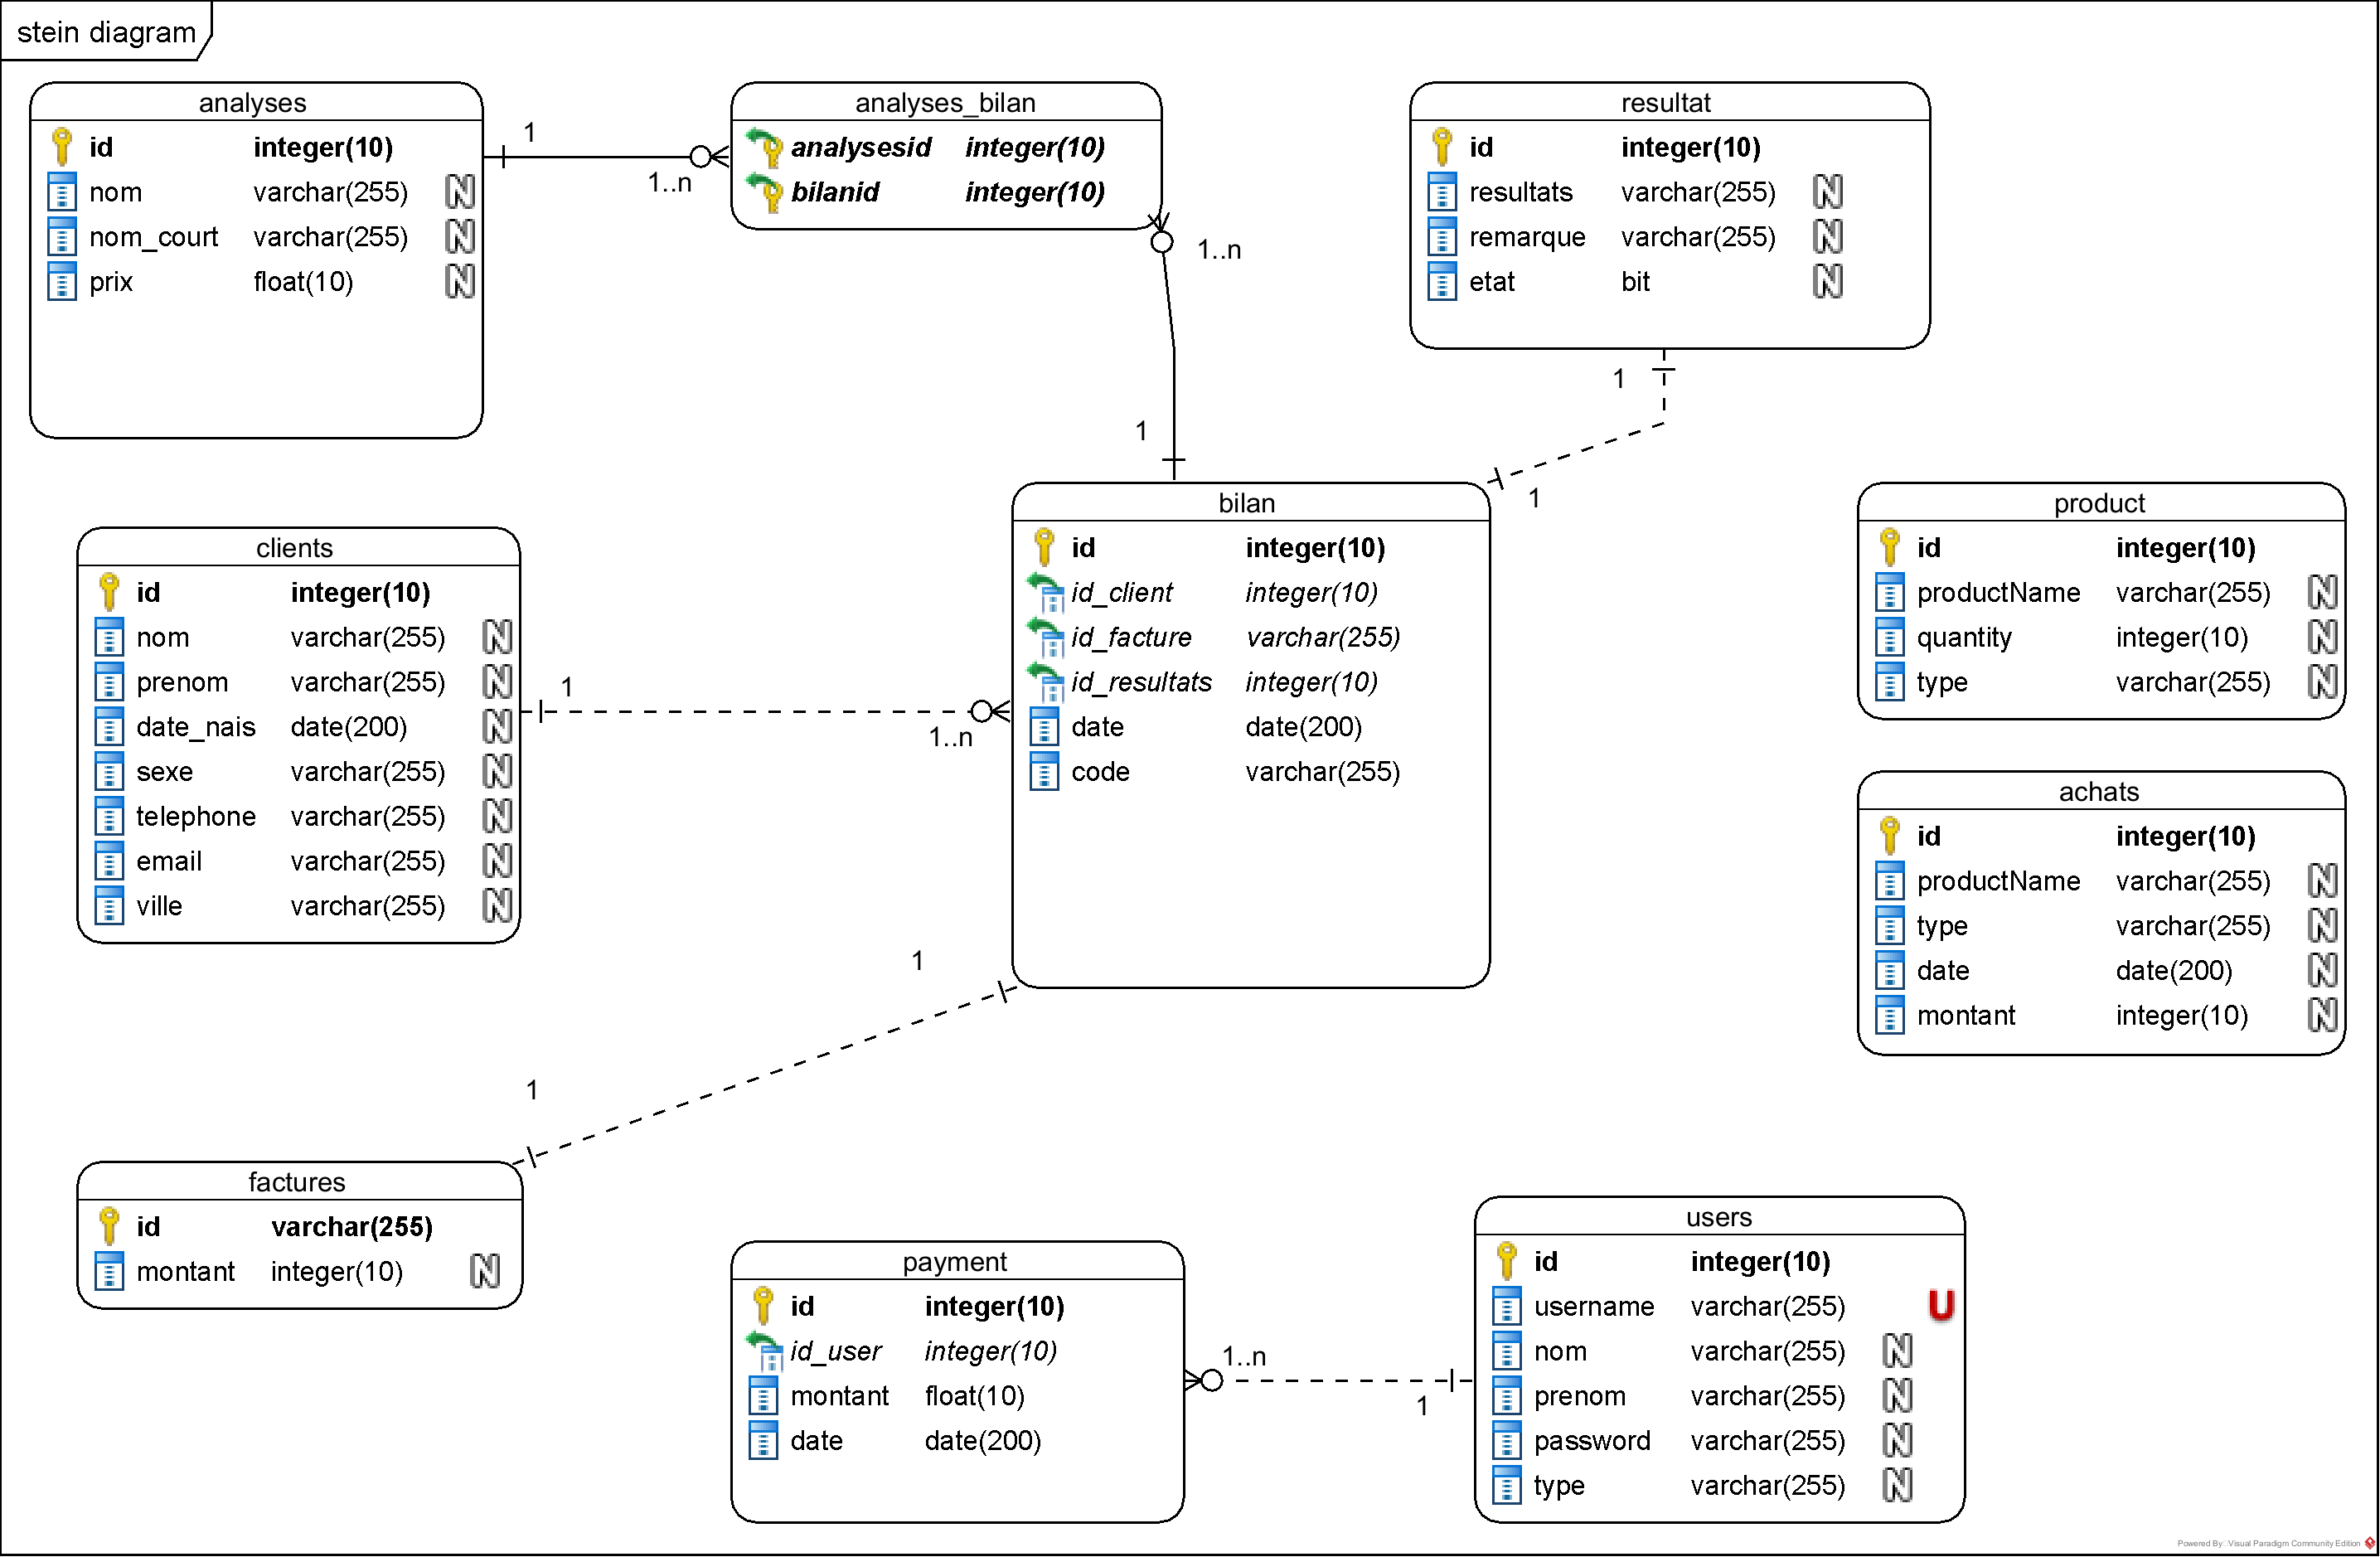
\includegraphics[width=451px]{media/entity relation diagram/database diagram.png}
    \captionof{figure}{Entity Relationship Diagram for Application Database}
\end{center}

\newpage
\subsection[Relational Model]{ER Diagram to Relational Model Transformation}
The transition from the DCL (Data Control Language) object model to the relational model is done with the aim of implementing the database as a relational DBMS (Database Management System). This transition is done by following a set of rules that allow the transformation of the object model into a relational model.

\subsubsection*{Rules of transformation:}

\begin{itemize}
    \item Each Entity is transformed into a table.
    \item Each column is kept as column.
    \item Each primary key is kept as primary key.
    \item Each relationship is transformed into a foreign key.
\end{itemize}

\subsubsection*{Relational Model:}

\begin{itemize}
    \item analyses (\underline{id}, nom, nom\_court, prix)
    \item clients (\underline{id}, nom, prenom, date\_nais, sexe, telephone, email, ville)
    \item bilan (\underline{id}, \dashuline{id\_client}, \dashuline{id\_facture}, \dashuline{id\_resultats}, date, code)
    \item analyse\_bilan (\dashuline{analysesid}, \dashuline{bilanid})
    \item facture(\underline{id}, montant)
    \item resultat (\underline{id}, resultats, remarque, etat)
    \item product (\underline{id}, productName, quantity, type)
    \item achats (\underline{id}, productName, type, date, montant)
    \item users(\underline{id}, username, nom, prenom, password, type)
    \item payment(\underline{id}, \dashuline{id\_user}, montant, date)
    
\end{itemize}

\subsection[Conclusion]{Conclusion}
In this section, we have used UML to design the application. We have created Use Case Diagrams, Sequence Diagrams, and Class Diagrams to represent the functionalities and structure of the system. 

We have also transformed the Class Diagram into a relational model to implement the database. 
In the next section, we will use this design to implement the application.

\newpage
\section[Application Implementation]{Application Implementation}
\subsection[Introduction]{Introduction}

After analyzing our needs and defining our project design methodology 
this section will be devoted to presenting the development tools and programming languages used for the implementation phase. 

This phase is based primarily on the results of the design and analysis phase. Each use case, sequence and detailed sequence diagrams defined in the analysis and design phase are put to use in the implementation phase with the help of appropriate technologies.

These technologies will be presented in this section, showcasing the architecture of the platform and illustrate screenshots of the interfaces used.

\subsection[Development environment]{Development environment}

\subsubsection*{IntelliJ IDEA:}

IntelliJ IDEA is an integrated development environment (IDE). It is a sophisticated and specialized IDE for Java and Kotlin development. It offers many tools and functionalities to maximize developer productivity.

We used IntelliJ IDEA as the main IDE for the development of our application.

\textit{Used version: IntelliJ IDEA 2024.1.1}

\subsection[Software]{Software}

\subsubsection*{XAMPP:}
The full form of XAMPP is “Cross-Platform (X), Apache (A), MySQL (M), PHP (P), and Perl (P).” This means that XAMPP is a tool that brings all these technologies together in one place.

\begin{center}
    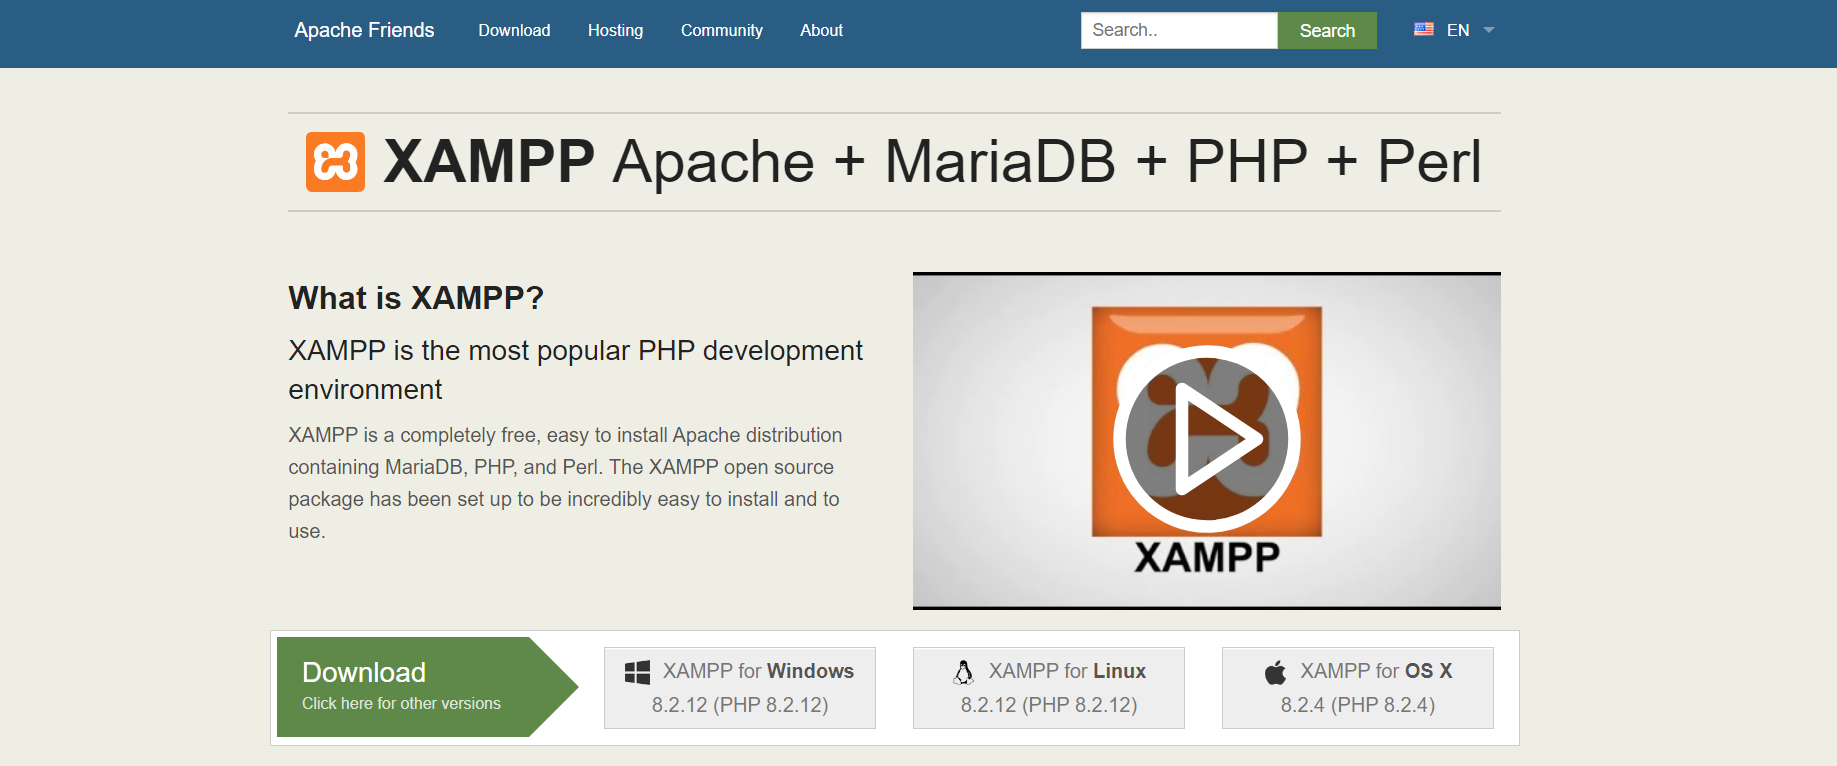
\includegraphics[width=451px]{media/xampp.png}
    \captionof{figure}{What is XAMPP?}
\end{center}

\begin{itemize}
    \item \textbf{Apache:} Apache is a web server that displays your website on the internet. The Apache server that comes with XAMPP provides you with local development.
    \item \textbf{MySQL:}\@ MySQL is an open-source relational database management system. You can use it to create a database and store data.
    \item \textbf{PHP:}\@ PHP is a server-side scripting language that helps in creating dynamic web applications. XAMPP also provides you PHP environment.
    \item \textbf{Perl:} Perl is a programming language used for server-side scripting.
\end{itemize}

XAMPP is a popular open-source web server package for website development. This gives you cross-platform functionality that allows you to easily use it on any platform. XAMPP is used in web development to set up a complete web server. XAMPP Supports multiple scripting languages. In addition, XAMPP also has the functions of an FTP server, Accelerated Mode, network download, etc.

We used XAMPP to set up a local server for our application in order to simulate the client-server environment required for our application. We also used it to create and manage the database.

\textit{Used version: XAMPP 8.2.4}


\subsubsection*{Figma:}
Figma is a web-based collaborative interface design tool that empowers teams to create and iterate on user interfaces (UIs) and user experiences (UX) for web, desktop, and mobile applications.

We used Figma to design the user interfaces of our application.

\textit{Used version: Figma 116.18.6}

\subsubsection*{Visual Paradigm:}
Visual Paradigm offers a variety of diagramming tools that use the Unified Modeling Language (UML) to create visual representations of software systems. This includes things like flowcharts, use case diagrams, and class diagrams. These diagrams help developers understand, design, and document complex systems.
It also goes beyond UML. While UML is a core strength, Visual Paradigm also supports other diagramming standards like mind maps and ER diagrams (entity-relationship diagrams) for broader project planning and data modeling.

We used Visual Paradigm for the application design phase to create UML diagrams.

\textit{Used version: Visual Paradigm CE 17.1}

\newpage
\subsection[Programming languages]{Programming languages}

\subsubsection*{Java:}
Java is a general-purpose, object-oriented programming language prized for its platform independence (write once, run anywhere) and focus on code reusability, security, and robustness. This makes it a powerful tool for developing a wide range of applications.

We used Java as the main programming language for the development of our application.

\textit{Used version: Java 17}

\subsubsection*{JavaFX:}
JavaFX is an open-source library for crafting desktop and rich internet applications (RIAs) with a focus on rich graphics, multimedia, and cross-platform compatibility.

We used JavaFX to create the graphical user interface (GUI) of our application.

\paragraph*{Main Characteristics:}

\begin{itemize}
    \item \textbf{Rich Graphics:} JavaFX provides a set of graphics and media packages that enable developers to create rich, interactive applications.
    \item \textbf{Cross-Platform Compatibility:} JavaFX applications can run on any platform that supports Java, including Windows, macOS, and Linux.
    \item \textbf{Scene Builder:} JavaFX includes a visual layout tool called Scene Builder that allows developers to design user interfaces by dragging and dropping components onto a canvas.
    \item \textbf{Modern UI with FXML and CSS:} JavaFX utilizes FXML, a declarative language similar to HTML, for defining the application's user interface (UI). This simplifies UI development and separation of concerns. Additionally, CSS allows for extensive customization of the application's look and feel.
\end{itemize}

\textit{Used version: JavaFX 17.0.6}

\subsection[Database Management System]{Database Management System}

\subsubsection*{MySQL:}

MySQL is an open-source relational database management system (RDBMS) that uses SQL (Structured Query Language) to manage and manipulate data. It is a popular choice for web applications and is widely used in conjunction with PHP to create dynamic websites.

We used MySQL as the database management system for our application with the help of XAMPP.

\textit{Used version: MySQL 15.1}
\newpage
\section[Project Presentation]{Project Presentation}
\subsection[Application Interfaces]{Application Interfaces}

\subsubsection*{Login Interface}
The main interface of the application is the login interface. It is where authentication takes place. The user must enter their username and password to access the application.
The user will be logged in as a laboratory manager, a doctor, a receptionist, or a biologist depending on the credentials they enter.
\begin{center}
    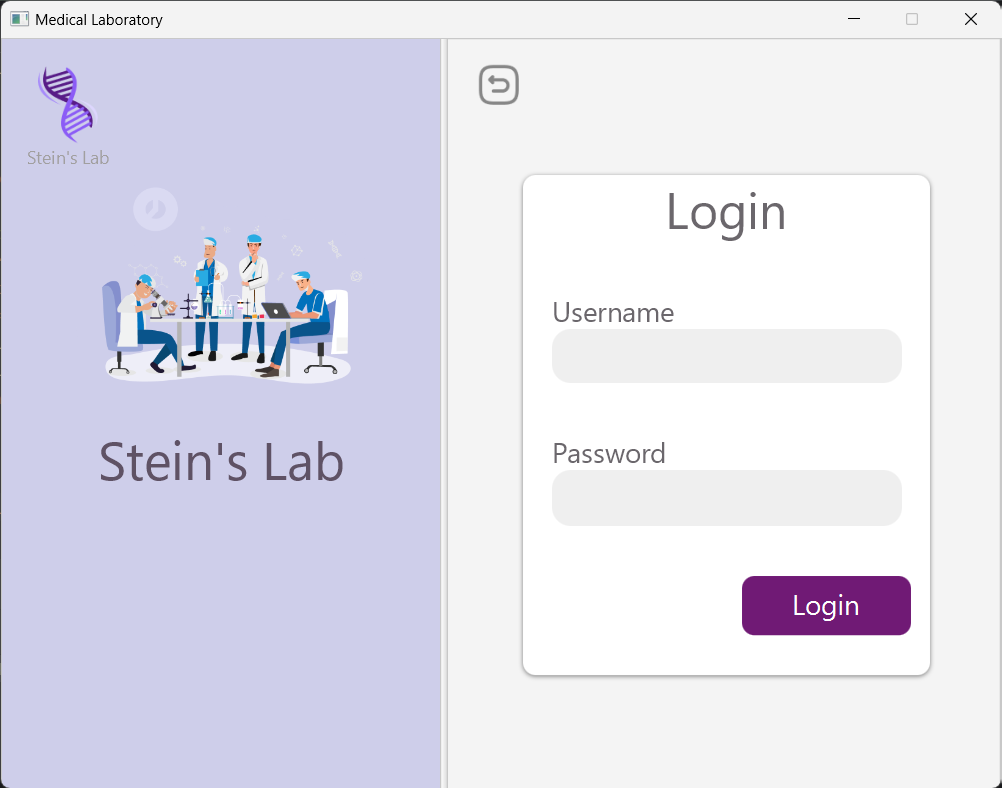
\includegraphics[width=451px]{media/interface/login.png}
    \captionof{figure}{Login Interface}
\end{center}

\newpage
\subsubsection*{Management of Employees Interface}
The management of employees interface allows the laboratory manager to manage the roles and privileges of each employee. The laboratory manager can add, modify, or delete an employee. The laboratory manager can also view the list of employees and their roles.
\begin{center}
    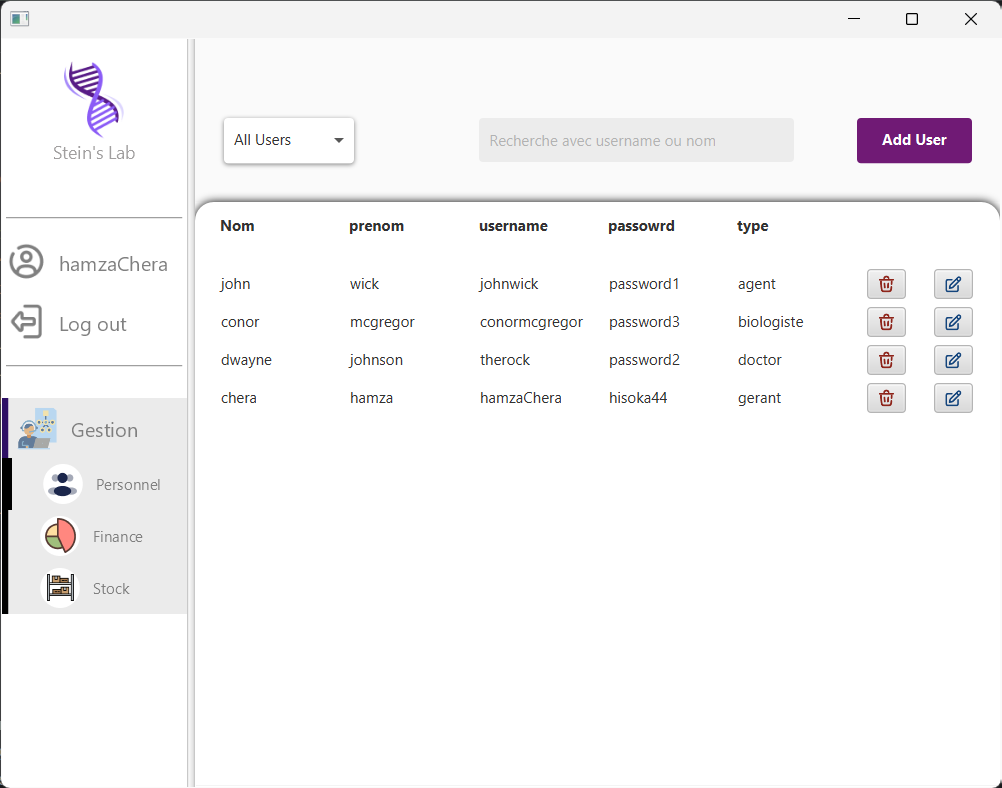
\includegraphics[width=451px]{media/interface/gestion personnel.png}
    \captionof{figure}{Management of Employees Interface}
\end{center}

\newpage
\subsubsection*{Management of Supply Interface}
The management of supply interface allows the laboratory manager to manage the supply of the laboratory. The laboratory manager can add, modify, or delete an equipment. The laboratory manager can also view the list of equipment and their quantity.
\begin{center}
    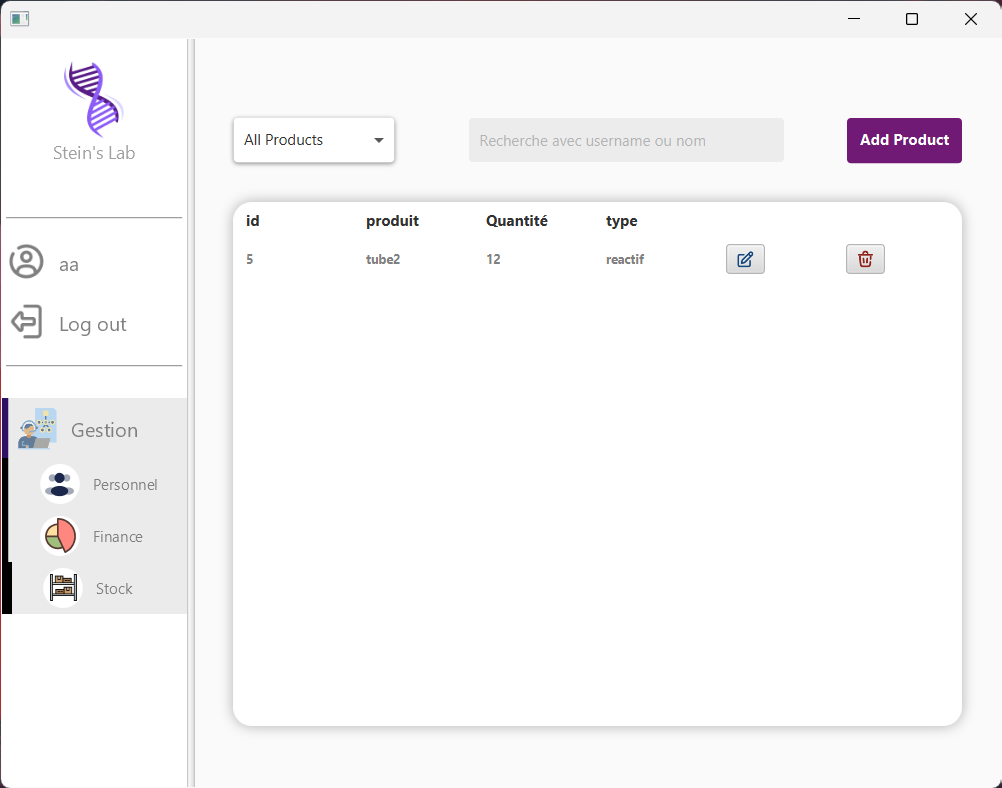
\includegraphics[width=451px]{media/interface/supply management.png}
    \captionof{figure}{Management of Supply Interface}
\end{center}

\newpage
\subsubsection*{Accounting Interface}
The accounting interface allows the laboratory manager to keep track of the financial situation of the laboratory. The laboratory manager can view the list of payments and purchases made by the laboratory as well as the income.
\begin{center}
    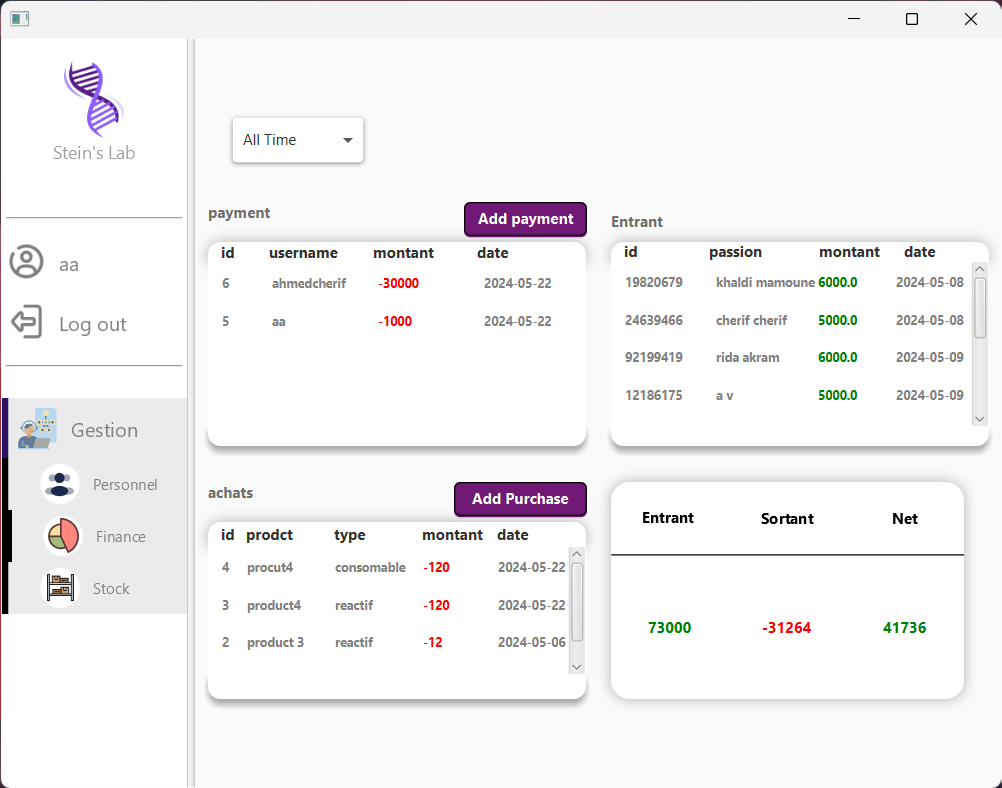
\includegraphics[width=451px]{media/interface/gestion finance.png}
    \captionof{figure}{Accounting Interface}
\end{center}

\newpage
\subsubsection*{Sample Management Interface}
The sample management interface allows the biologist to manage the sample test results of patients. The biologist can add or modify a sample test result. The biologist can also search for available samples.
\begin{center}
    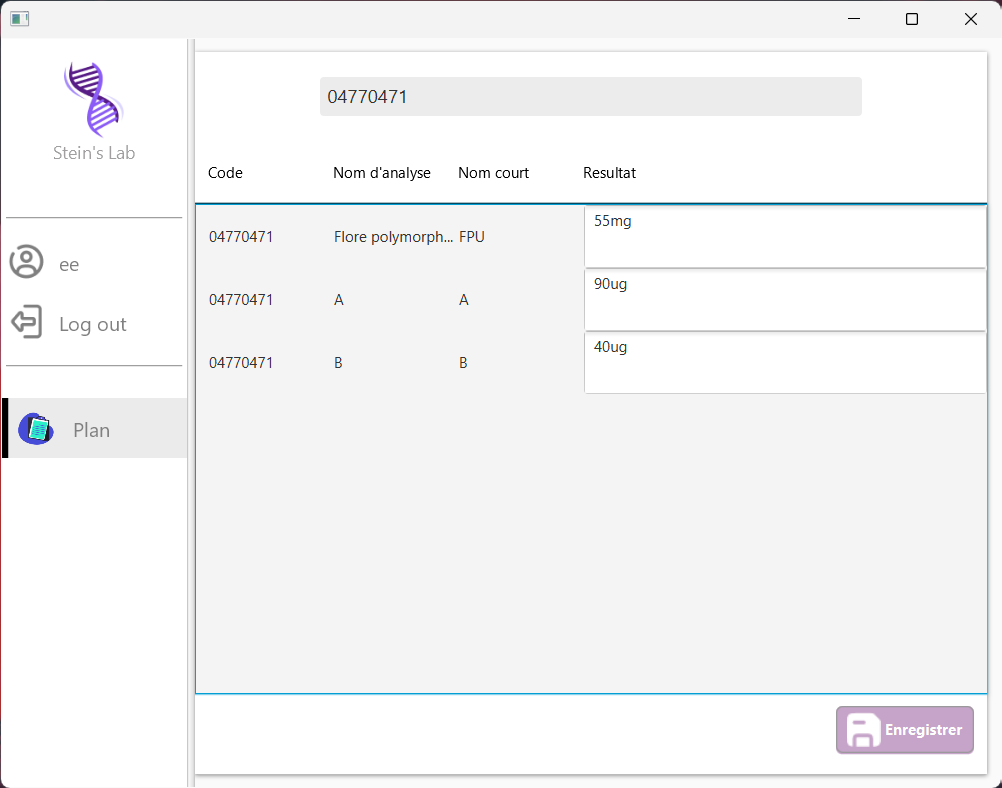
\includegraphics[width=451px]{media/interface/sample management.png}
    \captionof{figure}{Sample Management Interface}
\end{center}

\newpage
\subsubsection*{Results Validity Management Interface}
The results validity management interface allows the doctor to view the results of each patient's test and choose to validate those results for final delivery or not.
\begin{center}
    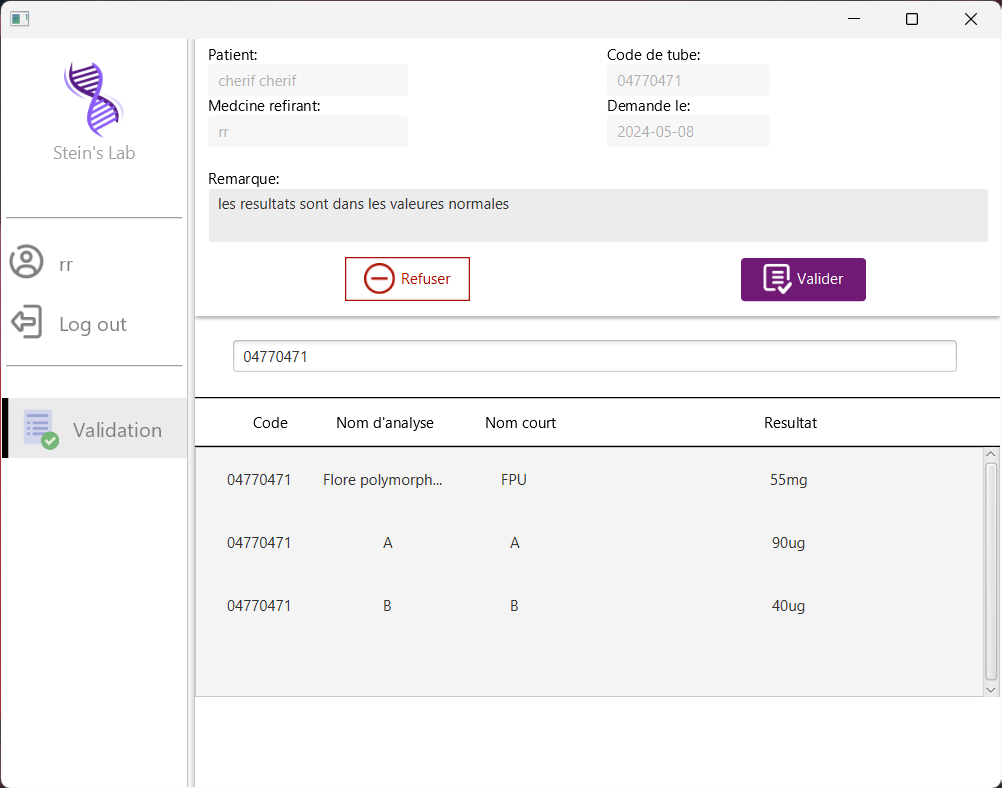
\includegraphics[width=451px]{media/interface/validation.png}
    \captionof{figure}{Results Validity Management Interface}
\end{center}

\newpage
\subsubsection*{Patients \& Medical Documents Management Interface}
The patients \& medical documents management interface allows the receptionist to store and manipulate patients data. The receptionist can add new patients and modify or delete existing ones. The receptionist can also search for available patients.
The interface also allows the receptionist to manage medical documents and relevant information for each patient.
\begin{center}
    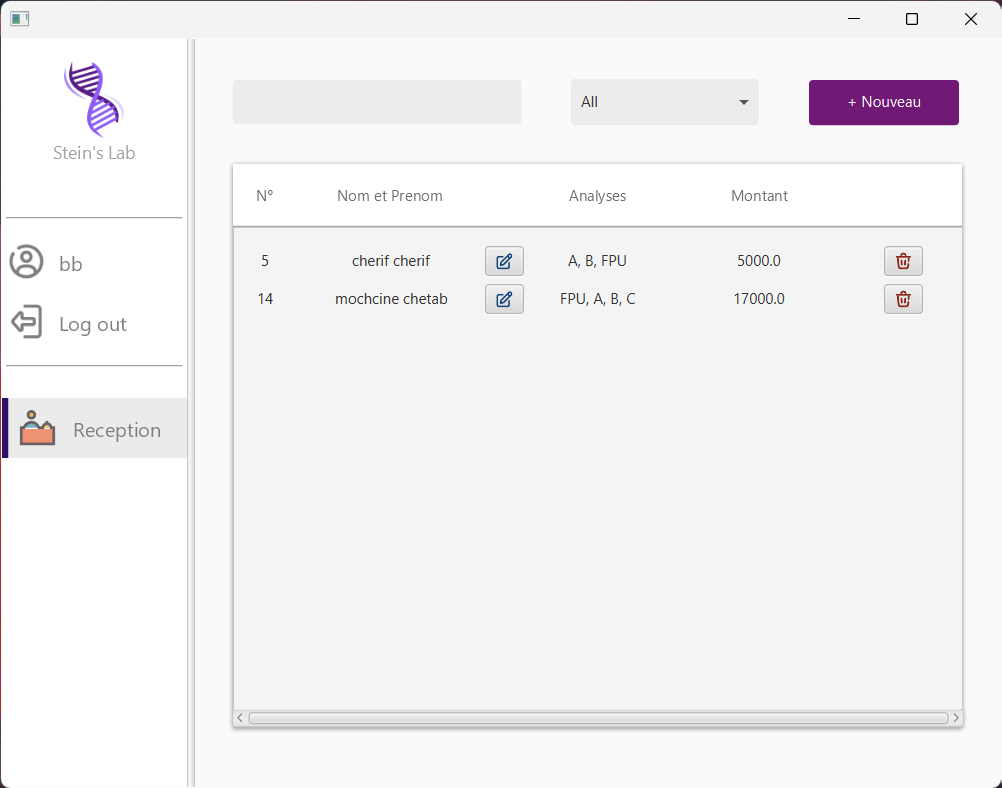
\includegraphics[width=451px]{media/interface/reception.png}
    \captionof{figure}{Patients Data Management Interface}
\end{center}

\newpage

\section[Conclusion]{Conclusion}
In this report, we have presented the development of an application for the management of a Medical Analysis Laboratory. We have described the purpose of the application, the existing solutions and their shortcomings, the requirements analysis, the application design, the application implementation, and the project presentation.

The realization of this project required good collaboration between our team members, as well as using best practices for software development.
Starting from requirements analysis then design.
Implementation required from us that we familiarize ourselves with many new technologies and methodologies.

We believe that our work will be of great benefit to the medical analysis laboratories that are looking for a reliable and easy-to-use software solution to manage their daily workflow.

We focused on bringing a simple and user friendly option to the market, as we noticed that most of the existing solutions are overcomplicated and lack attention to the user experience and user interface.

We hope that our application will help laboratories to improve their efficiency and productivity, and we look forward to receiving feedback from users to further improve our application.

\newpage

\section[References]{References}

\begin{itemize}
    \item \url{https://en.wikipedia.org/wiki/Unified_Modeling_Language}
    \item \url{https://en.wikipedia.org/wiki/IntelliJ_IDEA}
    \item \url{https://en.wikipedia.org/wiki/XAMPP}
    \item \url{https://en.wikipedia.org/wiki/Figma}
    \item \url{https://en.wikipedia.org/wiki/Java\_(programming\_language)}
    \item \url{https://en.wikipedia.org/wiki/JavaFX}
    \item \url{https://en.wikipedia.org/wiki/MySQL}
    \item \url{https://en.wikipedia.org/wiki/Relational_model}
    \item \url{https://en.wikipedia.org/wiki/Software_design}    
\end{itemize}


\end{document}